\documentclass[12pt, a4paper, reqno, oneside]{book}
\usepackage[left=2.5cm, right=2cm, top=2cm, bottom=2cm]{geometry}
\usepackage{amsmath,amsxtra,amssymb,latexsym, amscd,amsthm}
\usepackage{microtype}
\usepackage{indentfirst}
\usepackage{color}
\usepackage{empheq}
\usepackage{iftex}
\ifXeTeX
  \usepackage{fontspec}
  \setmainfont[Ligatures=TeX]{Times New Roman}
  \setsansfont[Ligatures=TeX]{Arial}
  \usepackage[vietnamese,english]{babel}
\else
  \usepackage[utf8]{inputenc}
  \usepackage[T5]{fontenc}
  \usepackage[vietnamese]{babel}
\fi
% \usepackage{amsmath} % đã được nạp ở dòng 3
\usepackage[mathscr]{eucal}
\usepackage{amsfonts}
\usepackage{graphicx}
\usepackage{float}
\usepackage{listings}
\usepackage[dvipsnames]{xcolor}
\usepackage{verbatim}
\usepackage{tikz}
\usetikzlibrary{calc,positioning,arrows.meta,shapes.geometric,fit,backgrounds,decorations.pathreplacing}
\usepackage{tkz-graph}
\usepackage{array}
\usepackage{multirow}
\usepackage{algorithm}
\usepackage{algpseudocode}
% Note: subfigure is legacy and conflicts with modern subcaption; kept commented for compatibility
% \usepackage{subfigure}
\usepackage{pgfplots}
\pgfplotsset{compat=1.18}
\usepackage{titlesec}
\usepackage{fancyhdr}
\usepackage{rotating}
\usepackage{longtable}
\usepackage{supertabular}
\usepackage{subcaption}
\usepackage{tabularx}
\usepackage[normalem]{ulem}
\usepackage{pdfpages}
\usepackage[square,numbers]{natbib}
\usepackage{booktabs}
\usepackage{chngcntr}
\usepackage{tabularray}
\usepackage{placeins}
\usepackage{enumitem}
\usepackage{seqsplit}
\usepackage{needspace}
\usepackage[labelfont=bf, textfont=it, justification=centering]{caption}
\captionsetup{labelfont={color=blue, bf}, textfont=it}
\captionsetup[table]{position=top}
\captionsetup[figure]{position=bottom}

\hyphenation{op-tical net-works semi-conduc-tor}
\usepackage[hyphens,spaces,obeyspaces]{url}
\usepackage{xurl}
\usepackage[colorlinks=true,bookmarksopen,bookmarksnumbered,citecolor=blue,linkcolor=blue,urlcolor=blue,pdftitle={Biểu diễn cấu trúc cho hệ thống phát hiện xâm nhập mạng CAN bus đa phương tiện},pdfauthor={Vũ Tiến Tuấn Trung}]{hyperref}
\def\UrlBreaks{\do\/\do-\do_\do.\do=\do?\do&\do~}
\def\UrlNoBreaks{\do\(\do\[\do\{\do\<\do\:}
\setlength{\emergencystretch}{1.5em}

\renewcommand{\baselinestretch}{1.25}
\setlength{\headheight}{15pt}
\setlength{\textfloatsep}{10pt plus 2pt minus 2pt}
\setlength{\intextsep}{8pt plus 2pt minus 2pt}
\setlength{\floatsep}{8pt plus 2pt minus 2pt}
\setlength{\abovecaptionskip}{4pt}
\setlength{\belowcaptionskip}{4pt}
\titleformat{\section}{\normalfont\Large\bfseries\raggedright}{\thesection}{1em}{}
\titleformat{\subsection}{\normalfont\large\bfseries\raggedright}{\thesubsection}{1em}{}

\fancyhf{}
\fancyhead[L]{\small{\leftmark}}
\fancyfoot[C]{\thepage}

\newcommand\chap[1]{%
  \clearpage\phantomsection%
  \chapter*{#1}%
  \addcontentsline{toc}{chapter}{#1}%
  \markboth{#1}{}%
}
\newcommand\sect[1]{%
  \Needspace{5\baselineskip}%
  \phantomsection%
  \addcontentsline{toc}{section}{#1}%
  \section*{#1}%
}

\renewcommand{\theequation}{\thechapter.\arabic{equation}}
\counterwithin{algorithm}{chapter}
\renewcommand{\thealgorithm}{\thechapter.\arabic{algorithm}}
\floatname{algorithm}{Thuật toán}
\renewcommand{\listalgorithmname}{Danh sách thuật toán}
\algrenewcommand\algorithmicrequire{\textbf{Đầu vào:}}
\algrenewcommand\algorithmicensure{\textbf{Đầu ra:}}
\newtheorem{lemma}{\bf Bổ đề}[chapter]
\newtheorem{theorem}{\bf Định lý}[chapter]
\newtheorem{proposition}{\bf Mệnh đề}[chapter]
\newtheorem{corollary}{\bf Hệ quả}[chapter]
\newtheorem{definition}{\bf Định nghĩa}[chapter]
\newtheorem{remark}{\bf Chú ý}[section]

% Mức tiêu đề sâu (subsubsubsection, paragraph)
\titleclass{\subsubsubsection}{straight}[\subsection]
\newcounter{subsubsubsection}[subsubsection]
\renewcommand\thesubsubsubsection{\thesubsubsection.\arabic{subsubsubsection}}
\renewcommand\theparagraph{\thesubsubsubsection.\arabic{paragraph}}

\titleformat{\subsubsubsection}
  {\normalfont\normalsize\bfseries}{\thesubsubsubsection}{1em}{}
\titlespacing*{\subsubsubsection}
  {0pt}{3.25ex plus 1ex minus .2ex}{1.5ex plus .2ex}

\makeatletter
\renewcommand\paragraph{\@startsection{paragraph}{5}{\z@}%
  {3.25ex \@plus1ex \@minus.2ex}%
  {-1em}%
  {\normalfont\normalsize\bfseries}}
\renewcommand\subparagraph{\@startsection{subparagraph}{6}{\parindent}%
  {3.25ex \@plus1ex \@minus .2ex}%
  {-1em}%
  {\normalfont\normalsize\bfseries}}
\def\toclevel@subsubsubsection{4}
\def\toclevel@paragraph{5}
\def\toclevel@paragraph{6}
\def\l@subsubsubsection{\@dottedtocline{4}{7em}{4em}}
\def\l@paragraph{\@dottedtocline{5}{10em}{5em}}
\def\l@subparagraph{\@dottedtocline{6}{14em}{6em}}
\makeatother

\setcounter{secnumdepth}{4}
\setcounter{tocdepth}{2}

% Thư mục hình ảnh
\graphicspath{{./figs/}}

\definecolor{mygreen}{rgb}{0,0.6,0}
\definecolor{mygray}{rgb}{0.5,0.5,0.5}
\definecolor{mymauve}{rgb}{0.58,0,0.82}

\lstdefinestyle{customc}{
  belowcaptionskip=1\baselineskip,
  breaklines=true,
  frame=single,
  xleftmargin=\parindent,
  language=C,
  showstringspaces=false,
  basicstyle=\footnotesize\ttfamily,
  keywordstyle=\bfseries\color{green!40!black},
  commentstyle=\itshape\color{purple!40!black},
  identifierstyle=\color{blue},
  stringstyle=\color{orange},
  numbers=left,
  numberstyle=\tiny\color{gray},
  stepnumber=1, 
}

\lstdefinestyle{customasm}{
  belowcaptionskip=1\baselineskip,
  frame=single,
  xleftmargin=\parindent,
  language=[x86masm]Assembler,
  basicstyle=\footnotesize\ttfamily,
  commentstyle=\itshape\color{purple!40!black},
  numbers=left,
  numberstyle=\tiny\color{gray},
  stepnumber=1, 
}

\lstset{escapechar=@,style=customc}

\definecolor{processblue}{cmyk}{0.96,0,0,0}
\newcolumntype{C}[1]{>{\centering\arraybackslash}p{#1}}
\definecolor{eclipseStrings}{RGB}{42,0.0,255}
\definecolor{eclipseKeywords}{RGB}{127,0,85}
\colorlet{numb}{magenta!60!black}

\lstdefinelanguage{json}{
    basicstyle=\normalfont\ttfamily,
    commentstyle=\color{eclipseStrings},
    stringstyle=\color{eclipseKeywords},
    numbers=left,
    numberstyle=\scriptsize,
    stepnumber=1,
    numbersep=8pt,
    showstringspaces=false,
    breaklines=true,
    frame=lines,
    string=[s]{"}{"},
    comment=[l]{:\ "},
    morecomment=[l]{:"},
    literate=
        *{0}{{{\color{numb}0}}}{1}
         {1}{{{\color{numb}1}}}{1}
         {2}{{{\color{numb}2}}}{1}
         {3}{{{\color{numb}3}}}{1}
         {4}{{{\color{numb}4}}}{1}
         {5}{{{\color{numb}5}}}{1}
         {6}{{{\color{numb}6}}}{1}
         {7}{{{\color{numb}7}}}{1}
         {8}{{{\color{numb}8}}}{1}
         {9}{{{\color{numb}9}}}{1}
}

\DeclareRobustCommand{\code}[1]{\nolinkurl{#1}}
\newcolumntype{Y}{>{\raggedright\arraybackslash}X}
\newcolumntype{P}[1]{>{\raggedright\arraybackslash}p{#1}}

\begin{document}
\hypersetup{pageanchor=false}
\selectlanguage{vietnamese}

% =========================================================================
% TRANG BÌA NGOÀI (BÌA CHÍNH - KHUNG ĐÔI TIKZ)
% =========================================================================
\begin{titlepage}
\begin{center}
	\begin{tikzpicture}[overlay,remember picture]
	    \draw [line width=3pt,rounded corners=0pt]
	        ($ (current page.north west) + (20mm,-20mm) $)
	        rectangle
	        ($ (current page.south east) + (-15mm,20mm) $);
	    \draw [line width=1pt,rounded corners=0pt]
	        ($ (current page.north west) + (21.5mm,-21.5mm) $)
	        rectangle
	        ($ (current page.south east) + (-16.5mm,21.5mm) $);
	\end{tikzpicture}
	\\[1mm]
    \centerline{\bf ĐẠI HỌC QUỐC GIA HÀ NỘI}
    \centerline{\bf TRƯỜNG ĐẠI HỌC CÔNG NGHỆ}
    
    \vspace*{1.8cm}
    \large
        \begin{figure}[H]
        \centering
        
\includegraphics[width=0.23\linewidth]{figs/uet.jpg}
        \end{figure}
    \vspace*{1cm}
    \centerline{\bf VŨ TIẾN TUẤN TRUNG}
    \vspace*{2.0cm}
    {\fontsize{15}{19}\selectfont\bfseries
    \centerline{BIỂU DIỄN CẤU TRÚC CHO HỆ THỐNG}
    \centerline{PHÁT HIỆN XÂM NHẬP MẠNG CAN BUS}
    \centerline{ĐA PHƯƠNG TIỆN\par}}
    \vspace*{2.2cm}
    \centerline{\bf KHÓA LUẬN TỐT NGHIỆP ĐẠI HỌC HỆ CHÍNH QUY}
    \vspace*{0.2cm}
    \centerline{\bf Ngành: Hệ thống thông tin}
    
    \vfill
    \centerline{\bf Hà Nội -- 2026}
    \vspace{13pt}
\end{center}
\end{titlepage}

\newpage

% =========================================================================
% TRANG BÌA PHỤ (BÌA TRONG - CÓ CÁN BỘ HƯỚNG DẪN)
% =========================================================================
\begin{titlepage}
\begin{center}
	\begin{tikzpicture}[overlay,remember picture]
	    \draw [line width=3pt,rounded corners=0pt]
	        ($ (current page.north west) + (20mm,-20mm) $)
	        rectangle
	        ($ (current page.south east) + (-15mm,20mm) $);
	    \draw [line width=1pt,rounded corners=0pt]
	        ($ (current page.north west) + (21.5mm,-21.5mm) $)
	        rectangle
	        ($ (current page.south east) + (-16.5mm,21.5mm) $);
	\end{tikzpicture}
	\\[1mm]
    \centerline{\bf ĐẠI HỌC QUỐC GIA HÀ NỘI}
    \centerline{\bf TRƯỜNG ĐẠI HỌC CÔNG NGHỆ}
    \vspace*{1.8cm}
    \large
        \begin{figure}[H]
        \centering
        
\includegraphics[width=0.23\linewidth]{figs/uet.jpg}
        \end{figure}
    \vspace*{0.9cm}
    \large
    \centerline{\bf VŨ TIẾN TUẤN TRUNG}
    \vspace*{1.8cm}
    {\fontsize{15}{19}\selectfont\bfseries
    \centerline{BIỂU DIỄN CẤU TRÚC CHO HỆ THỐNG}
    \centerline{PHÁT HIỆN XÂM NHẬP MẠNG CAN BUS}
    \centerline{ĐA PHƯƠNG TIỆN\par}}
    \vspace*{1.5cm}
    \centerline{\bf KHÓA LUẬN TỐT NGHIỆP ĐẠI HỌC HỆ CHÍNH QUY}
    \vspace*{0.2cm}
    \centerline{\bf Ngành: Hệ thống thông tin}
    
    \vspace*{1.4cm}
    \centerline{\bf Cán bộ hướng dẫn:}
    \centerline{\bf PGS. TS. Nguyễn Ngọc Hóa}
    
    \vfill
    \centerline{\bf Hà Nội -- 2026}
    \vspace{13pt}
\end{center}
\end{titlepage}

\newpage
\hypersetup{pageanchor=true}
\pagenumbering{roman}
\pagestyle{plain}

% =========================================================================
% LỜI CẢM ƠN
% =========================================================================
\chap{Lời cảm ơn}
\vspace{20pt}
Em xin bày tỏ lòng biết ơn sâu sắc tới thầy hướng dẫn, PGS. TS. Nguyễn Ngọc Hóa, vì sự tận tâm dìu dắt, những góp ý chuyên môn quý báu và sự động viên liên tục trong suốt quá trình nghiên cứu và thực hiện khóa luận. Kiến thức uyên bác, sự phản biện chặt chẽ và định hướng khoa học của thầy đã giúp em vượt qua nhiều thách thức phương pháp luận để hoàn thành công trình này.

Em cũng xin chân thành cảm ơn các nhóm tác giả và cộng đồng nghiên cứu an ninh mạng ô tô đã công bố công khai các bộ dữ liệu đối chuẩn và công trình khoa học về mạng CAN, tạo điều kiện thiết yếu cho quá trình đối chứng và kiểm chứng thực nghiệm của khóa luận.

Trong quá trình thực hiện, tác giả có sử dụng các công cụ hỗ trợ AI cho việc rà soát ngữ pháp, định dạng văn bản, đối chiếu tài liệu và gợi ý cú pháp lập trình. Tác giả đã trực tiếp kiểm tra mọi nguồn trích dẫn, thẩm định và xác nhận toàn bộ mã nguồn, tự tiến hành thực nghiệm và hoàn toàn chịu trách nhiệm đối với nội dung khoa học cuối cùng; mọi ý tưởng cốt lõi, thiết kế phương pháp, phân tích và kết luận trong khóa luận đều là công trình nghiên cứu độc lập của tác giả.

Dù đã nỗ lực tối đa để bảo đảm tính chặt chẽ học thuật, khóa luận khó tránh khỏi những hạn chế nhất định. Em rất mong nhận được những ý kiến đóng góp và nhận xét quý báu từ Hội đồng chấm khóa luận để hoàn thiện hơn nữa nghiên cứu trong tương lai.

Xin trân trọng cảm ơn!

\newpage

% =========================================================================
% LỜI CAM ĐOAN
% =========================================================================
\chap{Lời cam đoan}
\vspace{20pt}
Tôi xin cam đoan khóa luận tốt nghiệp này là công trình nghiên cứu độc lập của bản thân tôi, được thực hiện dưới sự hướng dẫn khoa học của PGS. TS. Nguyễn Ngọc Hóa. Tôi xác nhận rằng toàn bộ hoặc bất kỳ phần nào của khóa luận này chưa từng được nộp để xét cấp bằng tốt nghiệp hay bất kỳ bằng cấp, học vị nào khác tại Trường Đại học Công nghệ -- Đại học Quốc gia Hà Nội hay tại bất kỳ cơ sở giáo dục nào khác.

Mọi nguồn tài liệu tham khảo, dữ liệu, mã nguồn và công trình liên quan được sử dụng trong khóa luận đều đã được ghi nhận đầy đủ và trích dẫn đúng quy chuẩn. Tôi bảo đảm rằng toàn bộ số liệu thực nghiệm và các phân tích thống kê trình bày trong khóa luận là kết quả xác thực từ các thí nghiệm do tôi trực tiếp triển khai và kiểm chứng một cách độc lập, bảo đảm tính nghiêm ngặt và chính xác về mặt phương pháp luận.

Tôi xin cam kết bản cam đoan này được lập với tinh thần trung thực học thuật cao nhất và tuân thủ đầy đủ các quy chế, quy định đào tạo hiện hành của Trường Đại học Công nghệ, Đại học Quốc gia Hà Nội.

\begin{flushright}
{\it Tác giả khóa luận}
\hskip 1.5cm\quad

\vskip 2cm
{\bf Vũ Tiến Tuấn Trung}  \quad\ \quad
\end{flushright}

\newpage

% =========================================================================
% TÓM TẮT KHÓA LUẬN (VINAMESE)
% =========================================================================
\chap{Tóm tắt}
\vspace{-10pt}

Phát hiện xâm nhập trên mạng điều khiển cục bộ CAN (\textit{Controller Area Network}) khi chuyển giao sang các dòng xe chưa từng quan sát là thách thức lớn do định danh CAN-ID mang tính độc quyền theo từng nhà sản xuất. Khóa luận đề xuất và kiểm chứng thực nghiệm \textbf{khung phát hiện xâm nhập cấu trúc thích ứng ngưỡng gồm hai giai đoạn}, cho phép bộ mã hóa Transformer nhẹ (75.298 tham số) huấn luyện một lần trên xe nguồn có thể bảo vệ các dòng xe mới mà không cần dữ liệu tấn công có nhãn hay huấn luyện lại trọng số mạng nơ-ron.

Ở \textbf{Giai đoạn I (Biểu diễn cấu trúc độc lập định danh)}, hệ thống loại bỏ bit CAN-ID thô và tái định nghĩa định danh làm khóa truy xuất trạng thái nhân quả, tạo vector 30 chiều nắm bắt tần suất, thứ tự, chuyển tiếp và vi sai tải tin ($\Delta\text{payload}$). Đánh giá trên 4 tập chuyển giao CTT ở chế độ thuần nội dung cho thấy: tại ngưỡng tĩnh đóng băng từ nguồn, biểu diễn cấu trúc chưa cải thiện độ nhạy (Recall điều kiện B đạt 73,83\% so với 85,41\% của đầu vào thô) và trôi dạt ngưỡng nghiêm trọng ($\text{FAR} = 52{,}46\%$). Ngược lại, xét về xếp hạng độc lập ngưỡng, biểu diễn cấu trúc vượt trội rõ rệt khi nâng Average Precision (AP) từ 0,3781 lên 0,5554 (+17,74 điểm phần trăm ghép cặp). Với dữ liệu có dấu thời gian đơn điệu (136 bản ghi), biến thể động học thời gian 32 chiều nâng AP lên 0,9359 và hạ FAR nguồn xuống 2,46\% (vẫn vượt ngân sách 0,1\% tới 24,6 lần). Phép thăm dò tuyến tính chứng minh thuộc tính hình thái (đặc biệt là DLC và mặt nạ byte) vừa mã hóa danh tính hãng xe (đạt 94,88\% trên biểu diễn ẩn và 96,42\% từ riêng DLC--mặt nạ), vừa phân tách tấn công. Sự đan xen đặc trưng này khiến các kỹ thuật thích ứng cấp biểu diễn (MixStyle, LOVO-cAdv, LEACE/INLP8) không thể xóa ranh giới miền mà không làm suy giảm độ nhạy phát hiện.

Để khắc phục sụp đổ ngưỡng tĩnh mà không huấn luyện lại mô hình, \textbf{Giai đoạn II (Hiệu chuẩn nền lành tính và lọc sự kiện)} ước lượng ngưỡng phân vị ngoại mẫu từ tiền tố khởi động lành tính ($N_{\text{pool}} \in [3.539, 6.000]$ cửa sổ) kết hợp lọc trượt $m$-trong-$n$. Tại ngân sách danh định $\alpha = 1{,}0\%$, quy trình kiểm soát tốt tỷ lệ báo động giả thực nghiệm ($\le 1{,}08\%$, từ 0,22\% ở Tập 3 đến 2,00\% ở Tập 4) và khôi phục Recall điều kiện B đạt 40,42\%--48,59\% (vượt mức 33,73\% của đầu vào thô); lọc trượt 2-trong-3 tiếp tục hạ FAR trung bình xuống 0,22\% với Precision đạt 84,96\%. Trên dữ liệu ngoại bộ, hiệu chuẩn hạ FAR của DoS trên Opel Astra từ 31,53\% xuống 0,17\% (tại $\alpha = 0{,}1\%$) và triệt tiêu FAR về 0,00\% trên Renault Clio. So với các bộ phát hiện mật độ thuần xe đích (Mahalanobis ước lượng 1.890 tham số gây vỡ FAR đuôi gấp 5--15 lần), Transformer nguồn đóng băng đóng vai trò bộ nén rủi ro một chiều chỉ hiệu chuẩn duy nhất một ngưỡng vô hướng $\tau_{\text{target}}$, xác lập độ ổn định vượt trội khi vận hành.

\medskip
\noindent \textit{\textbf{Từ khóa:}} Mạng CAN, phát hiện xâm nhập, chuyển giao xuyên phương tiện, biểu diễn cấu trúc, hiệu chuẩn nền lành tính, an toàn ô tô.
\newpage

% =========================================================================
% TÓM TẮT KHÓA LUẬN (ENGLISH ABSTRACT)
% =========================================================================
\chap{Abstract}
\vspace{-10pt}

Intrusion detection on Controller Area Network (CAN) buses under cross-vehicle transfer to unseen platforms poses a formidable challenge due to manufacturer-proprietary CAN identifier (CAN-ID) assignments. This thesis proposes and empirically validates a \textbf{two-stage threshold-calibrated structural intrusion detection framework}, enabling a lightweight Transformer (75,298 parameters) trained once on source data to protect unseen platforms without labeled attacks or retraining.

In \textbf{Stage I (Identifier-Agnostic Structural Representation)}, raw CAN-ID bits are excluded and repurposed as causal lookup keys, yielding a 30-dimensional vector capturing frequency, order, sequential transitions, and same-ID payload differences ($\Delta\text{payload}$). Across four CTT transfer sets in a content-only regime, structural representations under static source-frozen thresholds do not enhance sensitivity (Condition B recall reaches 73.83\% vs. 85.41\% for raw inputs) and suffer severe threshold shift ($\text{FAR} = 52.46\%$). In threshold-independent ranking, however, structural features demonstrate clear superiority, raising Average Precision (AP) from 0.3781 to 0.5554 (+17.74 percentage points paired gain). With monotonic timestamps (136 clean captures), the 32-dimensional timed extension lifts AP to 0.9359 and reduces source FAR to 2.46\% (still 24.6-fold above the 0.1\% budget). Controlled linear probing reveals that syntax attributes (notably DLC and byte masks) simultaneously encode manufacturer identity (94.88\% probe accuracy on latents, 96.42\% from DLC--masks alone) and separate attacks. This feature entanglement prevents representation invariance methods (MixStyle, LOVO-cAdv, LEACE/INLP8) from removing domain boundaries without eroding sensitivity.

To overcome static threshold collapse without retraining, \textbf{Stage II (Benign Prefix Calibration and Event Filtering)} estimates an out-of-sample quantile threshold from unlabeled benign warmup prefixes ($N_{\text{pool}} \in [3{,}539, 6{,}000]$ windows) combined with an $m$-out-of-$n$ causal sliding filter. At nominal budget $\alpha = 1.0\%$, this protocol tightly controls empirical false alarm rates ($\le 1.08\%$, 0.22\%--2.00\%) and restores Condition B recall to 40.42\%--48.59\% (surpassing raw inputs' 33.73\%); 2-out-of-3 filtering further suppresses average FAR to 0.22\% with 84.96\% precision. On external benchmarks, calibration reduces Opel Astra DoS FAR from 31.53\% to 0.17\% (at $\alpha = 0.1\%$) and eliminates Renault Clio FAR to 0.00\%. Compared to target-only density estimators (where Mahalanobis fits 1,890 parameters causing tail FAR blowout of 5--15$\times$), the frozen source Transformer acts as a 1D risk compressor calibrating a single scalar threshold $\tau_{\text{target}}$, conferring superior operational stability.

\smallskip
\noindent \textit{\textbf{Keywords:}} CAN bus, intrusion detection, cross-vehicle transfer, structural representation, benign prefix calibration, automotive cybersecurity.
\newpage

% =========================================================================
% DANH MỤC (TOC, LOF, LOT, LOA, ABBREVIATIONS)
% =========================================================================
\begingroup
\small
\renewcommand{\baselinestretch}{0.95}\selectfont
\setlength{\parskip}{0pt}
\makeatletter
\renewcommand*\l@chapter[2]{%
  \ifnum \c@tocdepth >\m@ne
    \addpenalty{-\@highpenalty}%
    \vskip 0.25em \@plus\p@
    \setlength\@tempdima{1.5em}%
    \begingroup
      \parindent \z@ \rightskip \@pnumwidth
      \parfillskip -\@pnumwidth
      \leavevmode \bfseries
      \advance\leftskip\@tempdima
      \hskip -\leftskip
      #1\nobreak\hfil \nobreak\hb@xt@\@pnumwidth{\hss #2}\par
      \penalty\@highpenalty
    \endgroup
  \fi}
\makeatother
\tableofcontents
\endgroup
\clearpage

\clearpage
\begingroup
\small
\setlength{\parskip}{0pt}
\phantomsection
\addcontentsline{toc}{chapter}{Danh sách hình vẽ}
\listoffigures
\endgroup
\clearpage

\begingroup
\small
\setlength{\parskip}{0pt}
\phantomsection
\addcontentsline{toc}{chapter}{Danh sách bảng}
\listoftables
\endgroup
\clearpage

\begingroup
\small
\setlength{\parskip}{0pt}
\phantomsection
\addcontentsline{toc}{chapter}{Danh sách thuật toán}
\listofalgorithms
\endgroup
\clearpage

\chap{Danh mục từ viết tắt}
\vspace*{-12pt}
{\fontsize{8.5pt}{10.2pt}\selectfont\setlength{\tabcolsep}{3pt}\renewcommand{\arraystretch}{0.76}
\noindent\begin{tabularx}{\textwidth}{@{}lYlY@{}}
\toprule
\textbf{Ký hiệu} & \textbf{Ý nghĩa} & \textbf{Ký hiệu} & \textbf{Ý nghĩa} \\ \midrule
ACK & Acknowledgment (Xác nhận khung CAN) & INLP & Iterative Nullspace Projection (Chiếu không gian hạch) \\
AP & Average Precision (Độ chính xác trung bình) & LEACE & Least-Squares Concept Erasure (Triệt tiêu khái niệm L2) \\
cAdv & Conditional Adversarial (Đối kháng có điều kiện) & LOVO & Leave-One-Vehicle-Out (Giữ lại một xe kiểm thử) \\
CAN & Controller Area Network & LR & Logistic Regression (Hồi quy Logistic) \\
CAN-FD & CAN with Flexible Data-Rate & LRU & Least Recently Used (Thay thế ít dùng gần nhất) \\
CI & Confidence Interval (Khoảng tin cậy) & LSTM & Long Short-Term Memory \\
CRC & Cyclic Redundancy Check (Mã kiểm dư vòng) & MACs & Multiply-Accumulate Operations (Phép nhân-tích lũy) \\
CSMA/CD+AMP & CSMA / Collision Detection + AMP & MHA & Multi-Head Attention (Cơ chế chú ý đa đầu) \\
CTT & can-train-and-test (Bộ dữ liệu đối chuẩn) & MLM & Masked Language Modeling (Mô hình ngôn ngữ che) \\
DANN & Domain-Adversarial Neural Network & MLP & Multi-Layer Perceptron (Mạng nơ-ron đa tầng) \\
DBC & Database CAN (Cơ sở dữ liệu mô tả CAN) & OBD-II & On-Board Diagnostics II (Cổng chẩn đoán xe) \\
DKW & Dvoretzky--Kiefer--Wolfowitz (Bất đẳng thức chặn) & OOD & Out-of-Distribution (Ngoại phân phối) \\
DLC & Data Length Code (Mã độ dài dữ liệu) & PCA & Principal Component Analysis (Phân tích thành phần chính) \\
DNN & Deep Neural Network (Mạng nơ-ron sâu) & PR & Precision--Recall \\
DoS & Denial of Service (Từ chối dịch vụ) & PR-AUC & Diện tích dưới đường cong PR \\
E2E & End-to-End (Đầu cuối đến đầu cuối) & ROC-AUC & Diện tích dưới đường cong ROC \\
ECU & Electronic Control Unit (Bộ điều khiển điện tử) & ROM & Read-Only Memory (Bộ nhớ chỉ đọc / lưu tĩnh) \\
EOF & End of Frame (Kết thúc khung CAN) & RTR & Remote Transmission Request (Yêu cầu truyền từ xa) \\
FFN & Feed-Forward Network (Mạng truyền thẳng) & SHA-256 & Secure Hash Algorithm 256-bit \\
FLOPs & Floating Point Operations (Phép tính dấu phẩy động) & SOF & Start of Frame (Khởi đầu khung CAN) \\
F1 & Điểm F1 (Trung bình điều hòa Precision--Recall) & SRAM & Static Random Access Memory (RAM tĩnh) \\
FAR & False Alarm Rate (Tỷ lệ báo động giả) & TEC & Transmit Error Counter (Bộ đếm lỗi truyền) \\
FN/FP & False Negative / False Positive & TF & Transformer \\
FPR & False Positive Rate (Tỷ lệ dương tính giả) & TF-IDF & Term Frequency--Inverse Document Frequency \\
GRL & Gradient Reversal Layer (Tầng đảo gradient) & TN/TP & True Negative / True Positive \\
IDE & Identifier Extension bit (Bit mở rộng ID) & UDA & Unsupervised Domain Adaptation (Thích ứng miền) \\
IDS & Intrusion Detection System (Hệ thống phát hiện xâm nhập) & UET & Trường ĐH Công nghệ, ĐHQGHN \\
IFS & Interframe Space (Khoảng cách giữa các khung) & VNU & Đại học Quốc gia Hà Nội \\
IID & Indep. and Identically Distributed (Độc lập cùng PP) & & \\
\bottomrule
\end{tabularx}\par}
\addtocounter{table}{-1}

\newpage
\pagenumbering{arabic}
\pagestyle{fancy}



\chap{Mở đầu}\label{chap:introduction}

\sect{Bối cảnh và động cơ nghiên cứu}
Mạng điều khiển cục bộ CAN (\textit{Controller Area Network}) đóng vai trò là xương sống truyền thông nội mạng trên hầu hết các phương tiện giao thông đường bộ hiện đại, đảm bảo sự phối hợp thời gian thực giữa các bộ điều khiển điện tử (ECU) phụ trách hệ thống truyền lực, khung gầm, phanh và an toàn chủ động~\cite{bosch1991can,iso11898_1_2015}. Được thiết kế từ thập niên 1980 với mục tiêu tối ưu hóa chi phí cáp nối và độ trễ phân xử bus, giao thức CAN hoạt động theo cơ chế quảng bá không phân định địa chỉ nguồn--đích và hoàn toàn thiếu vắng các cơ chế bảo mật nền tảng như mã hóa nội dung hay xác thực tính toàn vẹn thông điệp~\cite{bozdal2020evaluation}. Khi các dòng xe hiện đại ngày càng mở rộng kết nối không dây, viễn thông (telematics) và hỗ trợ lái tự hành, bề mặt tấn công của phương tiện bị phơi bày nghiêm trọng. Các nghiên cứu an ninh ô tô kinh điển đã chứng minh rằng khi xâm nhập thành công vào một nút ngoại vi, kẻ tấn công có thể chèn các khung tin giả mạo để chiếm quyền điều khiển các chức năng vận hành cốt lõi, đe dọa trực tiếp đến tính mạng hành khách~\cite{koscher2010experimental,checkoway2011comprehensive}.

Để bảo vệ hạ tầng nội mạng mà không làm phát sinh chi phí đại tu phần cứng ECU hiện hữu, các hệ thống phát hiện xâm nhập (IDS) thụ động trên bus đã trở thành một giải pháp phòng vệ then chốt. Tuy nhiên, tính đặc thù độc quyền của ngành công nghiệp ô tô đặt ra một rào cản kỹ thuật nghiêm trọng: không gian truyền thông CAN được định nghĩa riêng biệt cho từng dòng xe thông qua ma trận định danh và cơ sở dữ liệu chuyển đổi (DBC file) do từng nhà sản xuất bảo mật nghiêm ngặt. Khi một mô hình IDS được huấn luyện tối ưu trên dữ liệu thu thập từ một mẫu xe nguồn tại phòng thí nghiệm, khả năng duy trì độ chính xác khi triển khai sang một dòng xe hoàn toàn mới (chuyển giao xuyên phương tiện -- \textit{cross-vehicle transfer}) thường suy giảm nghiêm trọng~\cite{koltai2026trust,lampe2024curated}. Thực trạng này đòi hỏi cộng đồng nghiên cứu phải chuyển dịch từ các mô hình học thuộc chữ ký tĩnh sang các phương pháp học biểu diễn có khả năng nắm bắt quy luật giao tiếp nội tại của giao thức, cho phép chuyển giao tri thức bảo mật giữa các nền tảng xe khác nhau mà không đòi hỏi thu thập dữ liệu tấn công có nhãn trên xe đích.

\sect{Các thách thức cốt lõi và khoảng trống nghiên cứu}
Qua khảo cứu toàn diện tài liệu nghiên cứu chuyên ngành, khóa luận nhận diện bốn khoảng trống nghiên cứu (Research Gaps) lớn đang cản trở việc phát triển các hệ thống IDS ô tô có năng lực chuyển giao thực tế:

\textbf{Khoảng trống 1: Sự phụ thuộc cứng vào không gian định danh độc quyền (Proprietary Identifier Dependency).} 
Phần lớn các nghiên cứu IDS ô tô ứng dụng học máy và học sâu hiện nay~\cite{song2020dcnn,won2026canbertplus,balasubramanian2025canlp} đều đưa trực tiếp mã định danh CAN-ID hoặc biểu diễn nhúng của CAN-ID vào các tầng nơ-ron phân loại. Do CAN-ID phản ánh trực tiếp kiến trúc phân xử và quyền ưu tiên riêng của từng hãng xe, không gian định danh giữa hai mẫu xe độc lập gần như không có sự giao thoa ngữ nghĩa. Khi đối mặt với dòng xe đích chưa từng quan sát trong tập huấn luyện, phân phối đầu vào của mô hình bị sụp đổ hoàn toàn, khiến hệ thống mất khả năng phân biệt lưu lượng bình thường và lưu lượng bất thường nếu không được gắn nhãn và huấn luyện lại từ đầu.

\textbf{Khoảng trống 2: Sự ngộ nhận giữa tính bất biến danh nghĩa và hiện tượng đan xen đặc trưng thực tế (Nominal Invariance vs. Feature Entanglement).}
Một số công trình gần đây đã cố gắng giải quyết sự phụ thuộc định danh bằng cách ẩn danh hóa hoặc loại bỏ hoàn toàn bit CAN-ID thô khỏi đầu vào~\cite{obafemi2026travel,khreasat2026relational}, với giả định rằng các đặc trưng cú pháp còn lại (độ dài dữ liệu DLC, chu kỳ xuất hiện, tần suất khung tin) sẽ tự động mang lại tính bất biến miền xe (vehicle-domain invariance). Tuy nhiên, các thuộc tính cú pháp này thực chất lại bị đan xen chặt chẽ (\textit{feature entanglement}) với đặc tính phần cứng và cấu hình mạng của từng hãng xe. Việc loại bỏ định danh một cách cảm tính mà không đo lường sự rò rỉ thông tin nền tảng có thể dẫn đến hai kịch bản cực đoan: hoặc mô hình vô tình học thuộc dấu ấn phần cứng của xe nguồn, hoặc biểu diễn bị triệt tiêu quá mức khiến năng lực phát hiện bất thường bị phá hủy hoàn toàn.

\textbf{Khoảng trống 3: Hiện tượng trôi dạt phân phối logit và sự sụp đổ của ngưỡng quyết định tĩnh (Logit Distribution Shift and Static Threshold Collapse).}
Trong các bài toán chuyển giao miền, sự biến thiên phân phối (dịch chuyển hiệp phương sai) và phân phối xác suất tiên nghiệm giữa các phương tiện (\textit{covariate and prior shift})~\cite{shimodaira2000covariate,morenotorres2012shift} dẫn đến sự trôi dạt nghiêm trọng của phân phối điểm số bất thường (logit shift) ở đầu ra mô hình. Nhiều công trình công bố chỉ báo cáo các chỉ số chất lượng xếp hạng độc lập ngưỡng như Diện tích dưới đường cong ROC (AUC) hoặc Độ chính xác trung bình (AP), từ đó đưa ra kết luận lạc quan về khả năng chuyển giao. Tuy nhiên, khi vận hành thực tế tại một ngưỡng phân loại đóng băng từ nguồn, sự trôi dạt logit khiến tỷ lệ báo động giả (FAR) bùng nổ vượt mức kiểm soát, rơi vào cái bẫy tỷ lệ nền (base-rate fallacy)~\cite{axelsson2000base,sommer2010outside} và làm tê liệt hệ thống cảnh báo của phương tiện.

\textbf{Khoảng trống 4: Sự thiếu vắng đối chứng sòng phẳng với các bộ phát hiện thuần đích (Lack of Fair Target-Only Baselines).}
Các nghiên cứu thích ứng miền hiện hành thường chỉ so sánh mô hình chuyển giao với chính mô hình nguồn chưa thích ứng, mà bỏ qua một câu hỏi phương pháp luận mang tính nền tảng: Dưới cùng một ngân sách quan sát dữ liệu khởi động hữu hạn trên xe đích, liệu việc chuyển giao một bộ mã hóa phức tạp từ nguồn có thực sự mang lại ưu thế vượt trội so với việc triển khai trực tiếp các thuật toán phát hiện mật độ thuần không giám sát trên miền đích (\textit{Target-Only unsupervised baselines}, chẳng hạn khoảng cách Mahalanobis OOD~\cite{lee2018mahalanobis})? Việc thiếu vắng các phép đối chứng sòng phẳng này khiến giá trị thực tiễn của các kiến trúc học chuyển giao nguồn chưa được khẳng định một cách thuyết phục.

Bài toán trọng tâm mà khóa luận giải quyết là thiết kế và kiểm chứng một khung biểu diễn cấu trúc độc lập định danh kết hợp cơ chế thích ứng ngưỡng không giám sát, cho phép một mô hình phát hiện xâm nhập huấn luyện một lần trên xe nguồn có thể chuyển giao hiệu quả sang các dòng xe chưa từng quan sát mà không cần dữ liệu tấn công có nhãn trên xe đích và không bị sụp đổ tỷ lệ báo động giả khi vận hành thực tế.

\sect{Mục tiêu và nhiệm vụ nghiên cứu}
Xuất phát từ bài toán trên, mục tiêu tổng quát của khóa luận là xây dựng, kiểm chứng thực nghiệm và chẩn đoán toàn diện một khung phát hiện xâm nhập dựa trên biểu diễn cấu trúc cho mạng CAN bus đa phương tiện, giải quyết đồng thời sự phụ thuộc vào bảng mã CAN-ID độc quyền và hiện tượng trôi dạt ngưỡng phân loại giữa các dòng xe.

Để đạt được mục tiêu duy nhất này, khóa luận triển khai năm nhiệm vụ nghiên cứu xuyên suốt:
\begin{enumerate}
    \item Hệ thống hóa nền tảng giao thức CAN 2.0A, các hình thái tấn công nội xe, bốn dạng dịch chuyển phân phối xuyên phương tiện và các khoảng trống phương pháp luận của các nghiên cứu IDS hiện hành.
    \item Thiết kế không gian biểu diễn cấu trúc 30 chiều độc lập định danh (cùng biến thể động học thời gian 32 chiều cho luồng đồng hồ chuẩn) kết hợp bộ mã hóa chuỗi Transformer gọn nhẹ (75.298 tham số).
    \item Xây dựng cơ chế hiệu chuẩn ngưỡng phân vị không giám sát trên tiền tố lành tính của xe đích kết hợp bộ lọc sự kiện trượt $m$-trong-$n$, đồng thời đối chứng với các kỹ thuật thích ứng cấp đặc trưng (MixStyle, đối kháng đa nguồn LOVO, làm trắng và triệt tiêu tuyến tính LEACE/INLP8) trong Chương~4 để làm rõ giới hạn của tính bất biến miền.
    \item Triển khai quy trình thực nghiệm đối chứng tái lập trên bộ đối chuẩn can-train-and-test (bốn cặp chuyển giao qua ba hạt giống ngẫu nhiên) và 57 bản ghi từ ba bộ dữ liệu ngoại bộ độc lập, kèm phân tích cắt bỏ và thăm dò tuyến tính có kiểm soát.
    \item Đánh giá khả năng khôi phục điểm vận hành, đối chứng công bằng với các bộ phát hiện mật độ thuần xe đích (Target-Only) dưới cùng ngân sách khởi động và kiểm toán chi phí tính toán cho bài toán giám sát thụ động.
\end{enumerate}

\sect{Phạm vi, đối tượng nghiên cứu và khung giải pháp hai giai đoạn}
Về phạm vi kỹ thuật, khóa luận tập trung vào bài toán phát hiện xâm nhập nhị phân (bình thường/tấn công) ở cấp cửa sổ rời rạc $W = 64$ khung tin trên giao thức CAN 2.0A (chuẩn định danh 11-bit) dưới mô hình quan sát thụ động chỉ đọc. Thuật ngữ \textit{đa phương tiện} trong tên đề tài được sử dụng theo nghĩa kỹ thuật ô tô, chỉ khả năng chuyển giao xuyên qua nhiều dòng xe và nền tảng phần cứng khác nhau (\textit{cross-vehicle / multi-vehicle}), không mang nghĩa truyền thông đa phương tiện (\textit{multimedia}).

Nhằm giải quyết đồng bộ bài toán phụ thuộc mã định danh và sự sụp đổ của ngưỡng phân loại tĩnh, khóa luận xây dựng \textbf{khung phát hiện xâm nhập cấu trúc thích ứng ngưỡng gồm hai giai đoạn cốt lõi}:
\begin{enumerate}
    \item \textbf{Giai đoạn I -- Học biểu diễn cấu trúc độc lập định danh và kiểm định zero-shot đóng băng:} Loại bỏ hoàn toàn bit CAN-ID thô khỏi đầu vào bộ mã hóa Transformer gọn nhẹ (75.298 tham số) và chuyển hóa định danh thành khóa truy xuất trạng thái nhân quả. Toàn bộ trọng số mạng và ngưỡng nguồn được đóng băng tuyệt đối khi đánh giá trên xe đích nhằm cô lập năng lực phân tách nội tại của không gian đặc trưng (đối chứng cả nhánh thuần nội dung 30 chiều và nhánh mở rộng động học thời gian 32 chiều trên luồng đồng hồ chuẩn).
    \item \textbf{Giai đoạn II -- Hiệu chuẩn ngưỡng vận hành trên tiền tố lành tính và lọc sự kiện:} Giữ nguyên toàn bộ trọng số bộ mã hóa nguồn (không huấn luyện lại), chỉ ước lượng một ngưỡng phân vị vô hướng duy nhất từ tiền tố khởi động lành tính không nhãn trên xe đích kết hợp bộ lọc sự kiện trượt $m$-trong-$n$ nhằm khắc phục sự trôi dạt phân phối điểm số và ổn định tỷ lệ báo động giả.
\end{enumerate}

Bên cạnh khung giải pháp chính hai giai đoạn, khóa luận tiến hành đối chứng có kiểm soát trong Chương~4 với các kỹ thuật thích ứng và triệt tiêu cấp biểu diễn (thăm dò tuyến tính Hewitt--Liang, MixStyle, học đa nguồn đối kháng LOVO và LEACE/INLP8) cùng các bộ phát hiện thuần xe đích, qua đó làm rõ hiện tượng đan xen đặc trưng và khẳng định tính tất yếu của cơ chế hiệu chuẩn ở Giai đoạn~II.

\sect{Các đóng góp chính của khóa luận}
Tương ứng với việc giải quyết bốn khoảng trống nghiên cứu đã nhận diện, khóa luận mang lại bốn đóng góp khoa học và thực nghiệm chính:
\begin{enumerate}
    \item \textbf{Thiết kế không gian biểu diễn cấu trúc 30 chiều độc lập định danh (Giai đoạn I):} Xây dựng quy trình trích xuất nhân quả cấp cửa sổ loại bỏ hoàn toàn các bit CAN-ID thô khỏi đầu vào bộ phân loại nhưng duy trì định danh làm khóa bảng lịch sử trạng thái gọn nhẹ (130 KiB RAM ở bản tham chiếu và nén còn $\approx 20{,}48$ KiB khi triển khai nhúng C/C++). Không gian 30 chiều nắm bắt đồng thời cú pháp khung tin, vi sai dữ liệu tải ($\Delta\text{payload}$) cùng định danh, thống kê phân xử cục bộ và cấu trúc chuyển tiếp liền kề, giúp nâng chất lượng xếp hạng độc lập ngưỡng (AP) ở điều kiện chuyển xe thêm +17,74 điểm phần trăm so với biểu diễn thô (và đạt $\text{AP} = 0{,}9359$ khi mở rộng sang biến thể động học thời gian 32 chiều trên luồng bus đồng hồ chuẩn).
    \item \textbf{Phân định lý luận và chẩn đoán thực nghiệm hiện tượng đan xen đặc trưng:} Thiết lập sự phân tách rõ ràng giữa \textit{tính bất biến dưới phép đổi tên định danh nhất quán} (một thuộc tính hình thức hẹp) với \textit{tính độc lập miền xe thực tế}. Thông qua thăm dò tuyến tính có đối chứng Hewitt--Liang và các thí nghiệm thích ứng cấp đặc trưng (MixStyle, học đối kháng đa nguồn LOVO, triệt tiêu tuyến tính LEACE/INLP8), khóa luận chứng minh các thuộc tính hình thái khung tin (độ dài DLC và mặt nạ byte) vừa chứa dấu ấn hãng xe sâu sắc (giải mã xe đạt 94,88\% trên biểu diễn ẩn và 96,42\% từ riêng DLC--mặt nạ), vừa là tín hiệu cốt lõi để phát hiện xâm nhập; do đó các kỹ thuật ép bất biến biểu diễn đơn thuần không thể triệt tiêu hoàn toàn ranh giới miền mà không làm suy giảm độ nhạy phát hiện.
    \item \textbf{Xây dựng cơ chế hiệu chuẩn tiền tố lành tính kết hợp lọc sự kiện trượt (Giai đoạn II):} Thiết kế quy trình hiệu chuẩn ngưỡng phân vị ngoại mẫu không giám sát từ tiền tố khởi động lành tính trên xe đích kết hợp bộ lọc sự kiện trượt $m$-trong-$n$, cho phép khôi phục điểm vận hành khả thi mà tuyệt đối không cần dữ liệu tấn công đích hay cập nhật trọng số mạng nơ-ron. Giải pháp kéo giảm tỷ lệ báo động giả trung bình từ trên 52\% về $\le 1{,}08\%$ tại ngân sách danh định $\alpha = 1{,}0\%$ (và xuống 0,22\% với Precision 84,96\% khi lọc 2-trong-3), đồng thời kiểm chứng hiệu quả khôi phục trên các tập dữ liệu ngoại bộ thực tế.
    \item \textbf{Thiết lập hệ thống đối chứng đa phương tiện tái lập và làm rõ lợi thế tham số so với mô hình thuần đích:} Triển khai bộ thực nghiệm kiểm chứng nghiêm ngặt qua 3 hạt giống ngẫu nhiên trên bộ đối chuẩn \textit{can-train-and-test} và 57 bản ghi từ ba bộ dữ liệu ngoại bộ độc lập. Phép đối chứng sòng phẳng dưới cùng ngân sách khởi động với các bộ phát hiện mật độ thuần xe đích (\textit{Target-Only}) làm sáng tỏ cơ chế bổ trợ kiến trúc: trong khi mô hình Mahalanobis phải ước lượng 1.890 tham số hiệp phương sai trực tiếp trên luồng đích không dừng dẫn tới vỡ FAR vùng đuôi gấp 5--15 lần, bộ mã hóa Transformer nguồn đóng băng đóng vai trò bộ nén rủi ro một chiều và chỉ hiệu chuẩn đúng một ngưỡng vô hướng, mang lại độ ổn định đuôi vượt trội trong vận hành thực tế.
\end{enumerate}

\sect{Tổ chức khóa luận}
Nội dung của khóa luận được tổ chức thành 4 chương chính và phần kết luận, với cấu trúc logic luân chuyển như sau:
\begin{itemize}
    \item \textbf{Chương~\ref{chap:background} (Cơ sở lý thuyết):} Trình bày nguyên lý hoạt động của mạng CAN, phân loại các mô hình tấn công trên bus, cơ sở toán học của bài toán dịch chuyển phân phối đa miền và nền tảng kiến trúc học biểu diễn chuỗi.
    \item \textbf{Chương~\ref{chap:related} (Các nghiên cứu liên quan):} Khảo cứu toàn diện các công trình IDS ô tô hiện hành, phân tích các phương pháp học chuyển giao và thích ứng miền, từ đó định vị rõ ràng các khoảng trống tri thức mà khóa luận tập trung giải quyết.
    \item \textbf{Chương~\ref{chap:method} (Khung biểu diễn cấu trúc xuyên phương tiện):} Định nghĩa hình thức mô hình đe dọa, đặc tả chi tiết thuật toán trích xuất biểu diễn cấu trúc 30 chiều, kiến trúc bộ mã hóa Transformer và quy trình hiệu chuẩn tiền tố lành tính gộp.
    \item \textbf{Chương 4 (Thực nghiệm và đánh giá):} Trình bày thiết lập thực nghiệm, đánh giá hiệu năng chuyển giao Giai đoạn~I và khôi phục vận hành Giai đoạn~II, phân tích cắt bỏ thành phần, đối chứng thích ứng miền, kiểm thử ngoại bộ và phân rã độ trễ thực thi.
    \item \textbf{\hyperref[chap:conclusion]{Kết luận và hướng phát triển}:} Đúc kết các kết luận khoa học cốt lõi, chỉ ra các giới hạn nội tại và đề xuất các định hướng nghiên cứu tiếp theo.
\end{itemize}

\chapter{Cơ sở lý thuyết}\label{chap:background}
Chương này thiết lập các nền tảng lý thuyết cốt lõi cho bài toán phát hiện xâm nhập mạng nội xe đa phương tiện, bao gồm kiến trúc tầng vật lý và cơ chế phân xử truy cập của giao thức CAN cùng mô hình quan sát thụ động của IDS, cơ chế tác động ở mức bus của các họ tấn công nội xe, bản chất chuyển dịch phân phối giữa các dòng xe cùng vai trò của các bộ dữ liệu đối chuẩn, và nền tảng toán học của học biểu diễn chuỗi tự chú ý dưới dịch chuyển miền.

\section{Giao thức mạng CAN và kiến trúc quan sát của IDS thụ động}
Mạng điều khiển cục bộ CAN (\textit{Controller Area Network}), do Robert Bosch GmbH đề xuất và chuẩn hóa quốc tế trong bộ tiêu chuẩn ISO~11898~\cite{bosch1991can,iso11898_1_2015,iso11898_2_2016}, đóng vai trò đường xương sống truyền thông thời gian thực kết nối các bộ điều khiển điện tử (\textit{Electronic Control Unit} --- ECU) trong ô tô hiện đại. Khác với các mạng chuyển mạch gói truyền thống, CAN hoạt động theo mô hình truyền thông hướng thông điệp (\textit{message-oriented}) trên môi trường đường truyền dùng chung: mỗi khung tin không mang địa chỉ trạm gửi hay trạm nhận tường minh mà chỉ mang một mã định danh phân xử (\textit{Arbitration ID}), vừa xác định ngữ nghĩa vật lý của dữ liệu vừa quy định mức độ ưu tiên truy cập bus.

\subsection{Đặc tính vật lý và truyền tín hiệu vi sai}
Theo chuẩn ISO~11898-2~\cite{iso11898_2_2016} (phổ biến $500\,\text{kbps}$ trên xe du lịch), các ECU kết nối song song qua cặp dây xoắn đôi vi sai \code{CAN_H} và \code{CAN_L} với hai điện trở kết cuối $120\,\Omega$ ở hai đầu trục nhằm triệt tiêu phản xạ sóng cao tần. Trạng thái logic trên bus được mã hóa qua hiệu điện thế vi sai $V_{\text{diff}} = V_{\text{CAN\_H}} - V_{\text{CAN\_L}}$ gồm hai mức đối nghịch:
\begin{itemize}
    \item \textbf{Trạng thái lặn (\textit{Recessive}, bit logic \texttt{1}):} $V_{\text{diff}} \approx 0\,\text{V}$ (hai dây cùng ở mức phân áp $\approx 2{,}5\,\text{V}$) khi không có nút nào chủ động phát.
    \item \textbf{Trạng thái trội (\textit{Dominant}, bit logic \texttt{0}):} $V_{\text{diff}} \approx +2{,}0\,\text{V}$ ($V_{\text{CAN\_H}} \approx 3{,}5\,\text{V}$ và $V_{\text{CAN\_L}} \approx 1{,}5\,\text{V}$) khi ít nhất một bộ thu phát kéo dòng chủ động.
\end{itemize}
Cơ chế vi sai giúp triệt tiêu nhiễu điện từ đồng pha trong khoang xe và tạo nền tảng cho phép toán logic wired-AND ở tầng liên kết dữ liệu.

\subsection{Cơ chế wired-AND và phân xử bit không phá hủy CSMA/CD+AMP}
Về mặt điện học, kết nối song song các bộ thu phát tạo nên phép toán \textbf{wired-AND} vật lý trên bus: chỉ cần một ECU phát mức trội (\texttt{0}) thì toàn bộ đường truyền lập tức bị kéo về trạng thái trội bất kể bao nhiêu ECU khác đang phát mức lặn (\texttt{1}); trạng thái lặn chỉ duy trì khi \emph{tất cả} các nút trên bus đều thả nổi ở mức \texttt{1}. Tính chất này là nền tảng cho cơ chế đa truy cập cảm nhận sóng mang kết hợp phát hiện xung đột và phân xử theo ưu tiên thông điệp (\textbf{CSMA/CD+AMP} --- \textit{Carrier Sense Multiple Access with Collision Detection and Arbitration on Message Priority})~\cite{bosch1991can,iso11898_1_2015}.

Cụ thể, sau khoảng nghỉ giữa các khung (\textit{Interframe Space} --- IFS gồm $3$ bit lặn), mọi ECU có dữ liệu chờ đều có thể đồng thời bắt đầu truyền bit khởi đầu khung trội (\textit{Start of Frame} --- SOF, giá trị \texttt{0}) để đồng bộ hóa cạnh xuống. Trong suốt pha truyền trường định danh (\textit{Arbitration Field}), từng nút đồng thời phát từng bit từ trọng số cao nhất (MSB) đến thấp nhất (LSB) và đọc ngược lại mức điện áp thực tế trên bus tại điểm lấy mẫu của mỗi chu kỳ bit $T_{\text{bit}}$ (chẳng hạn $T_{\text{bit}} = 2\,\mu\text{s}$ tại $500\,\text{kbps}$). Xét hai nút $a$ và $b$ cùng cạnh tranh đường truyền với hai mã định danh $11$ bit $c_a, c_b \in \{0, \ldots, 2047\}$, biểu diễn nhị phân $(c_{a,10}, \ldots, c_{a,0})_2$ và $(c_{b,10}, \ldots, c_{b,0})_2$. Gọi $k^*$ là vị trí bit có trọng số cao nhất nơi hai định danh khác nhau:
\begin{equation}\label{eq:can-arbitration}
k^* = \max\big\{k \in \{0, \ldots, 10\} : c_{a,k} \neq c_{b,k}\big\}.
\end{equation}
Tại chu kỳ bit tương ứng với $k^*$, nút có $c_{\cdot, k^*} = 0$ phát mức trội, còn nút có $c_{\cdot, k^*} = 1$ phát mức lặn nhưng đọc về mức trội trên bus. Ngay tại thời điểm phát hiện sai khác giữa bit gửi và bit đọc về, nút thua cuộc lập tức ngừng phát ở chu kỳ bit kế tiếp và chuyển sang chế độ chỉ nhận, trong khi nút thắng cuộc hoàn tất toàn bộ khung tin mà \emph{không hề bị hỏng dữ liệu hay phải truyền lại}. Do biểu diễn nhị phân quy ước \texttt{0} thắng \texttt{1}, mã định danh số học càng nhỏ thì quyền ưu tiên chiếm bus càng cao ($c_a < c_b \Rightarrow$ nút $a$ thắng).

\textbf{Giải thích vật lý của lỗ hổng từ chối dịch vụ (DoS):} Chính cơ chế phân xử không phá hủy theo thứ tự số học là nguyên nhân trực tiếp khiến bus CAN dễ tổn thương trước tấn công làm ngập. Khung tin mang mã định danh \texttt{0x000} gồm toàn bộ $11$ bit trội liên tiếp ($00000000000_2$). Bất kỳ lúc nào kẻ tấn công phát liên tục các khung \texttt{0x000} ngay khi bus vừa kết thúc $3$ bit \code{IFS}, mọi ECU hợp pháp mang định danh $c_i > 0$ đều chắc chắn thua phân xử ngay tại bit khác không đầu tiên của mình và phải lùi lại chờ khung tiếp theo. Một khung dữ liệu chuẩn CAN 2.0A có tổng chiều dài từ $44$ bit (\code{DLC}=0) đến $108$ bit (\code{DLC}=8) trước khi tính bit chèn (\textit{bit stuffing}, tối đa khoảng $20\%$), tức chỉ mất khoảng $88\text{--}260\,\mu\text{s}$ tại tốc độ $500\,\text{kbps}$. Do đó, việc bơm \texttt{0x000} với tần suất $4.000\text{--}10.000\text{ khung/giây}$ sẽ độc chiếm tuyệt đối băng thông vật lý, gây bỏ đói bus (\textit{bus starvation}) và trễ hạn thời gian thực đối với toàn bộ các hệ thống điều khiển có mức ưu tiên thấp hơn.

\subsection{Chuẩn CAN 2.0A (11 bit) so với CAN 2.0B (29 bit) và lỗ hổng bảo mật cấu trúc}
Đặc tả Bosch CAN 2.0 định nghĩa hai định dạng khung tin cùng tồn tại trên bus~\cite{bosch1991can,iso11898_1_2015}:
\begin{itemize}
    \item \textbf{Khung chuẩn CAN 2.0A (Base Frame, 11-bit ID):} Sử dụng $11$ bit định danh (tối đa $2^{11} = 2.048$ mã, từ \texttt{0x000} đến \texttt{0x7FF}) với bit mở rộng định danh \code{IDE = 0} (trội). Đây là định dạng phổ biến trên phần lớn các dòng xe du lịch thương mại và là phạm vi trực tiếp của khóa luận.
    \item \textbf{Khung mở rộng CAN 2.0B (Extended Frame, 29-bit ID):} Mở rộng không gian định danh lên $29$ bit ($2^{29}$ mã) bằng cách chèn bit \code{SRR} (\textit{Substitute Remote Request}, luôn ở mức lặn \texttt{1}), bit \code{IDE = 1} (lặn) và thêm $18$ bit định danh mở rộng sau phần $11$ bit cơ sở. Khi một khung 2.0A và 2.0B có cùng $11$ bit đầu cùng tranh chấp bus, khung 2.0A thắng phân xử nhờ bit \code{IDE = 0} trội ghi đè bit \code{IDE = 1} lặn.
\end{itemize}

Cấu trúc chi tiết các trường của một khung dữ liệu chuẩn CAN 2.0A $11$ bit cùng vai trò phân xử và mối liên hệ với đầu vào trích xuất đặc trưng của hệ thống IDS được minh họa trực quan tại Hình~\ref{fig:can-frame-11bit}.

\begin{figure}[htbp]
\centering
\begin{tikzpicture}[>=Stealth, font=\sffamily]
  % Total width = 15.4 cm (fits comfortably inside 16.5 cm \textwidth)
  \def\h{1.38}

  % Top group brackets
  \draw[decorate, decoration={brace, amplitude=4pt}, thick, blue!70!black] (0.02, \h+0.42) -- (4.18, \h+0.42)
    node[midway, above=5pt, font=\scriptsize\bfseries, text=blue!70!black] {Phân xử \& định danh (13 bit)};
  \draw[decorate, decoration={brace, amplitude=4pt}, thick, teal!70!black] (4.22, \h+0.42) -- (9.28, \h+0.42)
    node[midway, above=5pt, font=\scriptsize\bfseries, text=teal!70!black] {Điều khiển \& dữ liệu tải (6 -- 70 bit)};
  \draw[decorate, decoration={brace, amplitude=4pt}, thick, orange!70!black] (9.32, \h+0.42) -- (12.58, \h+0.42)
    node[midway, above=5pt, font=\scriptsize\bfseries, text=orange!75!black] {Toàn vẹn \& xác nhận (18 bit)};
  \draw[decorate, decoration={brace, amplitude=4pt}, thick, black!70] (12.62, \h+0.42) -- (15.38, \h+0.42)
    node[midway, above=5pt, font=\scriptsize\bfseries, text=black!80] {Kết thúc (10 bit)};

  % Bit lengths right above boxes
  \node[font=\tiny\bfseries] at (0.375, \h+0.18) {1b};
  \node[font=\tiny\bfseries] at (2.10,  \h+0.18) {11b};
  \node[font=\tiny\bfseries] at (3.825, \h+0.18) {1b};
  \node[font=\tiny\bfseries] at (5.20,  \h+0.18) {6b};
  \node[font=\tiny\bfseries] at (7.75,  \h+0.18) {0--64b (0--8B)};
  \node[font=\tiny\bfseries] at (10.10, \h+0.18) {15b};
  \node[font=\tiny\bfseries] at (11.175,\h+0.18) {1b};
  \node[font=\tiny\bfseries] at (11.75, \h+0.18) {1b};
  \node[font=\tiny\bfseries] at (12.325,\h+0.18) {1b};
  \node[font=\tiny\bfseries] at (13.425,\h+0.18) {7b};
  \node[font=\tiny\bfseries] at (14.825,\h+0.18) {3b};

  % SOF
  \filldraw[fill=red!18, draw=red!65!black, thick] (0.00,0) rectangle (0.75,\h);
  \node[align=center, font=\scriptsize\bfseries] at (0.375, 0.72) {SOF\\[-2pt]{\tiny (D=0)}};

  % 11-bit Arbitration ID
  \filldraw[fill=blue!16, draw=blue!70!black, thick] (0.75,0) rectangle (3.45,\h);
  \node[align=center, font=\scriptsize\bfseries] at (2.10, 0.70) {Arbitration ID\\[-1pt]{\tiny 11 bit (ID[10:0])}\\[-1pt]{\tiny $c_i \in [0, 2047]$}};

  % RTR
  \filldraw[fill=blue!10, draw=blue!70!black, thick] (3.45,0) rectangle (4.20,\h);
  \node[align=center, font=\scriptsize\bfseries] at (3.825, 0.70) {RTR\\[-2pt]{\tiny (0/1)}};

  % Control (6b)
  \filldraw[fill=cyan!14, draw=teal!75!black, thick] (4.20, 0.92) rectangle (6.20, \h);
  \node[font=\scriptsize\bfseries] at (5.20, 1.15) {Control (6b)};
  \filldraw[fill=cyan!8, draw=teal!75!black, thick] (4.20, 0) rectangle (4.75, 0.92);
  \node[rotate=90, font=\tiny\bfseries] at (4.475, 0.46) {IDE (1b)};
  \filldraw[fill=cyan!8, draw=teal!75!black, thick] (4.75, 0) rectangle (5.25, 0.92);
  \node[rotate=90, font=\tiny\bfseries] at (5.00, 0.46) {r0 (1b)};
  \filldraw[fill=teal!20, draw=teal!75!black, thick] (5.25, 0) rectangle (6.20, 0.92);
  \node[align=center, font=\scriptsize\bfseries] at (5.725, 0.46) {DLC\\[-2pt]{\tiny 4b ($d_i$)}};

  % Data Field
  \filldraw[fill=teal!14, draw=teal!75!black, thick] (6.20,0) rectangle (9.30,\h);
  \node[align=center, font=\scriptsize\bfseries] at (7.75, 0.70) {Data Field (Payload)\\[-1pt]{\tiny 0--8 Byte ($\mathbf{b}_i$)}\\[-1pt]{\tiny $m_{i,j}=\mathbf{1}[j<d_i]$}};

  % CRC Seq (15b) + Del (1b)
  \filldraw[fill=orange!15, draw=orange!75!black, thick] (9.30,0) rectangle (10.90,\h);
  \node[align=center, font=\scriptsize\bfseries] at (10.10, 0.70) {CRC Seq.\\[-1pt]{\tiny 15 bit}};
  \filldraw[fill=orange!24, draw=orange!75!black, thick] (10.90,0) rectangle (11.45,\h);
  \node[rotate=90, font=\tiny\bfseries] at (11.175, 0.69) {CRC Del (R)};

  % ACK Slot (1b) + Del (1b)
  \filldraw[fill=yellow!22, draw=orange!75!black, thick] (11.45,0) rectangle (12.05,\h);
  \node[rotate=90, font=\tiny\bfseries] at (11.75, 0.69) {ACK Slot};
  \filldraw[fill=orange!24, draw=orange!75!black, thick] (12.05,0) rectangle (12.60,\h);
  \node[rotate=90, font=\tiny\bfseries] at (12.325, 0.69) {ACK Del (R)};

  % EOF (7b)
  \filldraw[fill=gray!18, draw=black!75, thick] (12.60,0) rectangle (14.25,\h);
  \node[align=center, font=\scriptsize\bfseries] at (13.425, 0.70) {EOF\\[-1pt]{\tiny 7 bit (R=1)}};

  % IFS (3b)
  \filldraw[fill=gray!10, draw=black!65, dashed, thick] (14.25,0) rectangle (15.40,\h);
  \node[align=center, font=\scriptsize\bfseries] at (14.825, 0.70) {IFS\\[-1pt]{\tiny 3 bit (R=1)}};

  % Bottom extraction mapping annotations
  \draw[->, thick, blue!70!black] (2.10, -0.05) -- (2.10, -0.52);
  \draw[->, thick, teal!75!black] (5.725, -0.05) -- (5.725, -0.52);
  \draw[->, thick, teal!75!black] (7.75, -0.05) -- (7.75, -0.52);

  \node[draw=blue!55!black, fill=blue!5, rounded corners=3pt, align=center, font=\scriptsize, text width=14.9cm, inner sep=4pt]
    (idsmap) at (7.70, -1.08) {%
      \textbf{Ánh xạ sang bộ trích xuất đặc trưng IDS:} Khung quan sát $F_i=(t_i,c_i,d_i,\mathbf{b}_i,y_i)$ sử dụng trường \textbf{Arbitration ID} ($c_i$), \textbf{DLC} ($d_i$) và \textbf{Data Field} ($\mathbf{b}_i$). Các mô hình truyền thống đưa trực tiếp bit $c_i$ vào phân loại; trong khi tiếp cận cấu trúc loại bỏ định danh tuyệt đối khỏi đầu vào trực tiếp và sử dụng $c_i$ làm khóa tra cứu ngữ cảnh và động học luồng tin.%
    };

  % Compact legend line
  \node[font=\tiny, anchor=north west, text=black!80] at ([yshift=-6pt]idsmap.south west)
    {Chú thích mức vật lý: \textbf{D=0} -- bit trội ($V_{\text{diff}}\approx 2\,\text{V}$); \textbf{R=1} -- bit lặn ($V_{\text{diff}}\approx 0\,\text{V}$); \textbf{Del} -- bit phân tách (\textit{Delimiter}); \textbf{EOF} -- kết thúc khung; \textbf{IFS} -- khoảng nghỉ giữa hai khung.};
\end{tikzpicture}
\caption[Cấu trúc khung dữ liệu chuẩn CAN 2.0A (11-bit) và ánh xạ trường thông tin IDS]{Cấu trúc khung dữ liệu chuẩn CAN 2.0A ($11$-bit Arbitration ID) theo ISO~11898-1 và mối liên hệ giữa các trường khung tin với đầu vào của hệ thống IDS.}\label{fig:can-frame-11bit}
\end{figure}

Từ góc độ an toàn thông tin, thiết kế nguyên thủy của CAN 2.0A/B ưu tiên tối đa tính tất định thời gian thực và chi phí phần cứng thấp, dẫn đến năm lỗ hổng bảo mật cấu trúc cố hữu~\cite{bozdal2020evaluation,koscher2010experimental,checkoway2011comprehensive}:
\begin{enumerate}
    \item \textbf{Môi trường truyền thông quảng bá (\textit{broadcast medium}):} Mọi khung tin truyền trên bus đều lan truyền đồng thời tới tất cả các nút thu phát, không có cơ chế cách ly cổng vật lý theo cặp nguồn--đích. Một ECU hoặc thiết bị chẩn đoán bị xâm nhập có thể nghe lén toàn bộ lưu lượng trên nhánh bus đó.
    \item \textbf{Thiếu trường địa chỉ nguồn và đích:} Mã định danh $c_i$ chỉ đại diện cho loại thông điệp và mức ưu tiên phân xử, hoàn toàn không xác định danh tính phần cứng của ECU phát. Mọi nút trên bus đều có thể phát khung tin mang bất kỳ giá trị $c_i$ hợp lệ nào mà giao thức tầng liên kết dữ liệu không thể phân biệt nguồn phát thật hay giả.
    \item \textbf{Không có mã xác thực thông điệp (\textit{no authentication / MAC}):} Trường kiểm tra \code{CRC} $15$ bit chỉ phát hiện lỗi truyền dẫn ngẫu nhiên (nhiễu điện từ), không có giá trị bảo mật mật mã. Dung lượng tải cực hạn $0\text{--}8$ byte của CAN cổ điển cũng gây trở ngại lớn cho việc chèn chữ ký số hay mã xác thực MAC truyền thống trên các phần cứng di sản.
    \item \textbf{Không có mã hóa nội dung tải (\textit{no encryption}):} Toàn bộ $8$ byte dữ liệu $\mathbf{b}_i$ truyền dưới dạng bản rõ, cho phép kẻ tấn công giải mã ngược bảng ánh xạ tín hiệu DBC hoặc phát hiện quy luật biến thiên vật lý của xe.
    \item \textbf{Không có bộ đếm tươi hay chống phát lại (\textit{no freshness / anti-replay}):} Khung CAN chuẩn không chứa số thứ tự hay nhãn thời gian xác thực, nên kẻ tấn công có thể ghi lại các khung hợp lệ (như mở khóa cửa, chuyển số, phanh) và phát lại tùy ý.
\end{enumerate}

\subsection{Mô hình quan sát thụ động và biểu diễn khung tin}
Trong bối cảnh không thể thay thế đồng loạt toàn bộ các ECU di sản để triển khai xác thực mật mã, hệ thống phát hiện xâm nhập (IDS) thụ động đóng vai trò lớp phòng thủ giám sát bổ trợ không xâm lấn. IDS trong nghiên cứu quan sát bản ghi khung tin sau khi truyền trên bus, không can thiệp vào quá trình phân xử và không quan sát trực tiếp mọi trạng thái vật lý nội bộ của từng ECU. Ngoài ra, chênh lệch thời gian ghi nhận trong nhật ký lưu lượng còn phụ thuộc phần cứng thu, độ phân giải timestamp và tải tức thời của bus; vì vậy không được diễn giải máy móc mọi thay đổi nhịp thời gian là hành vi tấn công~\cite{bozdal2020evaluation,verma2024road}.

Ký hiệu khung tin thứ $i$ quan sát được trên luồng CAN là
\begin{equation}\label{eq:can-frame}
F_i=(t_i,c_i,d_i,\mathbf{b}_i,y_i),\quad d_i\in\{0,\ldots,8\},\quad y_i\in\{0,1\},
\end{equation}
trong đó $t_i$ là timestamp, $c_i \in \{0,\ldots,2047\}$ là mã định danh chuẩn 11 bit, $d_i$ là số byte hữu hiệu (\code{DLC}), $\mathbf{b}_i=(b_{i,0},\ldots,b_{i,7}) \in \{0,\ldots,255\}^8$ là vector payload đã đệm $0$ ngoài phạm vi $d_i$, và $y_i$ là nhãn nhị phân sau khi kiểm tra chính sách gán nhãn của từng bộ dữ liệu. Cần lưu ý rằng $t_i$ là siêu dữ liệu do thiết bị thu ghi lại chứ không phải trường dữ liệu được xác thực trong khung tin; đồng thời mặt nạ tính hợp lệ $m_{i,j} = \mathbf{1}[j < d_i]$ được dùng để phân biệt byte đệm mang giá trị $0$ với byte dữ liệu thực sự mang giá trị $0$.

\section{Các cơ chế tấn công trên mạng nội xe}
Trên môi trường đường truyền quảng bá thiếu xác thực nguồn, kẻ tấn công khi chiếm quyền một ECU hoặc kết nối thiết bị độc hại qua cổng chẩn đoán OBD-II/giao diện không dây có thể chèn, sửa đổi hoặc triệt tiêu lưu lượng CAN~\cite{koscher2010experimental,checkoway2011comprehensive}. Nghiên cứu giả định mô hình IDS thụ động chỉ đọc luồng khung tin mà không chủ động chặn gói hay phát khung lỗi phá hủy; đồng thời tấn công sửa đồng thời cả log thu và nhãn chuẩn (ground truth) nằm ngoài phạm vi đánh giá. Dựa trên đặc trưng vật lý và tác động lên chuỗi thông điệp trong các bộ dữ liệu đối chuẩn, bốn họ tấn công trọng tâm được phân tích chi tiết như sau:

\begin{enumerate}
    \item \textbf{Tấn công từ chối dịch vụ / Làm ngập bus (\textit{DoS / Flooding}):} Kẻ tấn công khai thác trực tiếp cơ chế phân xử bit trội CSMA/CD+AMP bằng cách phát liên tục các khung tin có mã định danh ưu tiên tuyệt đối (thường là \texttt{0x000} hoặc các ID rất thấp) ngay sau mỗi chu kỳ nghỉ \code{IFS}. Vì mọi bit của \texttt{0x000} đều ở mức trội, nút tấn công thắng phân xử trong mọi cuộc cạnh tranh, đẩy hiệu suất chiếm dụng bus lên gần $100\%$, làm tăng đột biến tần suất cục bộ $f_k(\texttt{0x000})$, ép số định danh phân biệt trong cửa sổ $U_k$ giảm mạnh và làm trễ hạn hoặc mất hoàn toàn các khung điều khiển chu kỳ thấp hơn của các ECU hợp pháp. Về mặt dữ liệu, cần lưu ý chính sách tạo mẫu của từng bộ benchmark: chẳng hạn với Automotive v2, đoạn tấn công DoS được tạo bằng cách thay thế một khoảng thời gian trong bản sao trace bình thường~\cite{dupont2019automotive} chứ không phải chèn thêm song song toàn bộ lưu lượng thực.
    \item \textbf{Tấn công dò quét ngẫu nhiên (\textit{Fuzzing}):} Kẻ tấn công bơm các khung tin mang mã định danh $c_i$ ngẫu nhiên hoặc quét tuần tự trên không gian 11 bit (bao gồm cả các ID chưa từng xuất hiện trong từ điển hợp lệ $\mathcal{C}_v$ của xe) kết hợp với độ dài $d_i$ và các byte dữ liệu $\mathbf{b}_i$ ngẫu nhiên có entropy cao. Trên bus, luồng fuzzing phá vỡ cấu trúc định danh ổn định của cửa sổ: số ID phân biệt $U_k$ tăng vọt, ma trận chuyển tiếp liên tiếp $T_k(c_{i-1}, c_i)$ xuất hiện nhiều cặp chuyển tiếp bất thường, còn giá trị $|\Delta \mathbf{b}_i|$ tại các ID trùng ngẫu nhiên dao động hỗn loạn. Ở mức vật lý, các khung fuzzing không hợp lệ có thể kích hoạt trạng thái bất thường trên bảng điều khiển hoặc phát sinh khung lỗi từ các ECU nhận.
    \item \textbf{Tấn công giả mạo / Chèn có chủ đích (\textit{Spoofing / Injection}):} Kẻ tấn công nhắm vào một mã định danh chức năng cụ thể $c^* \in \mathcal{C}_v$ (như vòng tua máy \code{rpm}, tốc độ \code{speed}, trạng thái số \code{force-neutral}, hoặc các kịch bản chèn theo chu kỳ \code{interval}, \code{double}, \code{triple}, \code{systematic} trong \texttt{can-train-and-test}~\cite{lampe2024curated}) để truyền các giá trị payload giả mạo $\mathbf{b}_{\text{adv}}$ mà không vô hiệu hóa ECU gốc. Hệ quả trên bus là cuộc \emph{đua thời gian} (\textit{timing race}): các khung giả mạo xen kẽ giữa chu kỳ tự nhiên $\Delta t_{c^*}$ của ECU thật, làm tần suất $f_k(c^*)$ tăng gấp đôi hoặc hơn, tạo ra các cặp tự chuyển tiếp $(c^*, c^*)$ bất thường trong $T_k$, và gây ra bước nhảy vi sai payload $|b_{i,j} - b_{q,j}|$ đột ngột khi giá trị thật và giả đan xen liên tiếp. Tuy nhiên, với các cuộc tấn công giả mạo biến thiên chậm hoặc chỉ thay đổi nhẹ một vài bit/byte biên (\code{force-neutral}, \code{speed}), biên độ tín hiệu vi sai rất nhỏ và dễ lẫn vào nhiễu vận hành bình thường.
    \item \textbf{Tấn công đình chỉ và mạo danh (\textit{Suspension / Masquerade}):} Đây là hình thái tấn công tinh vi gồm hai pha liên tiếp nhằm triệt tiêu hiện tượng xung đột payload giữa khung thật và khung giả:
    \begin{itemize}
        \item Ở pha \textit{Đình chỉ (Suspension)}, kẻ tấn công làm câm lặng ECU hợp pháp phát mã $c^*$ — có thể thông qua cơ chế ép lỗi \textbf{Bus-Off} theo ISO~11898-1 (liên tục ghi đè bit trội lên các bit lặn trong trường dữ liệu hoặc CRC của nạn nhân để đẩy bộ đếm lỗi phát \textit{Transmit Error Counter} vượt ngưỡng $\text{TEC} > 255$, buộc ECU nạn nhân tự ngắt khỏi bus) hoặc vô hiệu hóa phát tại nút bị chiếm quyền. Khi chỉ có pha đình chỉ (như trong bộ dữ liệu CAN-MIRGU~\cite{rajapaksha2024canmirgu}), trên bus không xuất hiện bất kỳ khung độc hại nào được chèn thêm mà chỉ ghi nhận sự biến mất của $c^*$ ($f_k(c^*) \to 0$) trong suốt khoảng đình chỉ được gán nhãn $1$. Vì vậy, trong phân tích CAN-MIRGU, nhãn từng khung tin được trích xuất trực tiếp từ cột nhãn tường minh ở cuối dòng thay vì giả định mọi khung trong tệp tấn công đều là khung độc hại được chèn.
        \item Ở pha \textit{Mạo danh (Masquerade)}, sau khi ECU gốc đã bị triệt tiêu, nút tấn công tiếp quản và phát các khung giả mạo mang mã $c^*$ đúng theo chu kỳ danh định $\Delta t_{c^*}$ của nạn nhân. Nhờ đó, mật độ tần suất $f_k(c^*)$, số ID phân biệt $U_k$ và thậm chí chuỗi chuyển tiếp ID gần như không đổi so với bình thường, khiến mọi bộ phát hiện chỉ dựa vào ID hoặc nhịp thời gian đều bị qua mặt; dấu vết còn lại chủ yếu nằm ở sự bất nhất cục bộ của payload và vi sai $\Delta \mathbf{b}_i$ so với ngữ cảnh vận hành các ID lân cận.
    \end{itemize}
\end{enumerate}

Đối với dữ liệu mô phỏng hoặc bản ghi đã qua chỉnh sửa hậu kỳ, mọi kết luận thực nghiệm trong khóa luận chỉ phát biểu về dấu vết quan sát được trên luồng bus mà không suy diễn sang tác động cơ học ngoài thực tế. Hình~\ref{fig:attack-passive-ids} đối chiếu trực quan bốn hình thái tấn công nói trên trên trục thời gian CAN cùng mô hình triển khai bộ phát hiện IDS thụ động tại cổng trung tâm (Central Gateway / cổng chẩn đoán OBD-II).

\begin{figure}[htbp]
\centering
\begin{tikzpicture}[>=Stealth, font=\sffamily]
  % ==================== PANEL (a): Bus Timeline of 4 Attack Families ====================
  \draw[rounded corners=4pt, draw=black!45, fill=gray!3] (0.0, 0.0) rectangle (15.4, -7.05);
  \node[anchor=north west, font=\footnotesize\bfseries, text=black!85] at (0.18, -0.14)
    {(a) Đối chiếu hình thái bốn họ tấn công trên trục thời gian khung tin CAN};

  \draw[->, thick, black!60] (3.45, -1.12) -- (15.05, -1.12) node[right, font=\tiny\bfseries] {$t$};
  \node[font=\tiny, text=black!75] at (5.90, -0.90) {Chu kỳ $\Delta t_{\texttt{0x240}}$};
  \draw[<->, thin, black!60] (4.70, -1.12) -- (7.10, -1.12);

  % Row 1: Normal (y=-1.70)
  \node[anchor=west, font=\scriptsize\bfseries, text=teal!75!black] at (0.18, -1.70) {0. Bình thường};
  \draw[thin, gray!45] (3.45, -1.70) -- (14.95, -1.70);
  \foreach \x/\id in {3.60/0x120, 4.70/0x240, 5.80/0x310, 7.10/0x120, 8.20/0x240, 9.30/0x310, 10.60/0x120, 11.70/0x240, 12.80/0x310, 14.00/0x120} {
    \filldraw[fill=teal!18, draw=teal!70!black, rounded corners=1.5pt] (\x, -1.92) rectangle (\x+0.88, -1.48);
    \node[font=\tiny\bfseries] at (\x+0.44, -1.70) {\texttt{\id}};
  }

  % Row 2: DoS / Flooding (y=-2.80)
  \node[anchor=west, font=\scriptsize\bfseries, text=red!75!black] at (0.18, -2.80) {1. DoS / Làm ngập};
  \draw[thin, gray!45] (3.45, -2.80) -- (12.60, -2.80);
  \filldraw[fill=teal!18, draw=teal!70!black, rounded corners=1.5pt] (3.60, -3.02) rectangle (4.48, -2.58);
  \node[font=\tiny\bfseries] at (4.04, -2.80) {\texttt{0x120}};
  \foreach \x in {4.60, 5.48, 6.36, 7.24, 8.12, 9.00, 9.88, 10.76, 11.64} {
    \filldraw[fill=red!24, draw=red!75!black, rounded corners=1.5pt] (\x, -3.02) rectangle (\x+0.80, -2.58);
    \node[font=\tiny\bfseries, text=red!75!black] at (\x+0.40, -2.80) {\texttt{0x000}};
  }
  \node[draw=red!60!black, dashed, fill=white, rounded corners=1.5pt, font=\tiny, text=red!75!black, inner sep=2.5pt]
    at (13.85, -2.80) {Bỏ đói ECU ($c_i > 0$)};

  % Row 3: Fuzzing (y=-3.90)
  \node[anchor=west, font=\scriptsize\bfseries, text=orange!80!black] at (0.18, -3.90) {2. Fuzzing};
  \draw[thin, gray!45] (3.45, -3.90) -- (11.45, -3.90);
  \filldraw[fill=teal!18, draw=teal!70!black, rounded corners=1.5pt] (3.60, -4.12) rectangle (4.48, -3.68);
  \node[font=\tiny\bfseries] at (4.04, -3.90) {\texttt{0x120}};
  \filldraw[fill=orange!26, draw=orange!80!black, rounded corners=1.5pt] (4.70, -4.12) rectangle (5.68, -3.68);
  \node[font=\tiny\bfseries] at (5.19, -3.90) {\texttt{0x7A3}?};
  \filldraw[fill=orange!26, draw=orange!80!black, rounded corners=1.5pt] (5.86, -4.12) rectangle (6.58, -3.68);
  \node[font=\tiny\bfseries] at (6.22, -3.90) {\texttt{0x4F1}};
  \filldraw[fill=teal!18, draw=teal!70!black, rounded corners=1.5pt] (7.10, -4.12) rectangle (7.98, -3.68);
  \node[font=\tiny\bfseries] at (7.54, -3.90) {\texttt{0x240}};
  \filldraw[fill=orange!26, draw=orange!80!black, rounded corners=1.5pt] (8.16, -4.12) rectangle (9.22, -3.68);
  \node[font=\tiny\bfseries] at (8.69, -3.90) {\texttt{0x6C9}?};
  \filldraw[fill=orange!26, draw=orange!80!black, rounded corners=1.5pt] (9.40, -4.12) rectangle (10.28, -3.68);
  \node[font=\tiny\bfseries] at (9.84, -3.90) {\texttt{0x5E2}};
  \filldraw[fill=teal!18, draw=teal!70!black, rounded corners=1.5pt] (10.48, -4.12) rectangle (11.36, -3.68);
  \node[font=\tiny\bfseries] at (10.92, -3.90) {\texttt{0x310}};
  \node[font=\tiny, text=orange!80!black, anchor=west, fill=gray!3, inner sep=2pt] at (11.55, -3.90) {ID lạ ($U_k\uparrow$), DLC/Payload hỗn loạn};

  % Row 4: Spoofing / Injection (y=-5.00)
  \node[anchor=west, font=\scriptsize\bfseries, text=purple!75!black] at (0.18, -5.00) {3. Spoofing / Chèn};
  \draw[thin, gray!45] (3.45, -5.00) -- (10.25, -5.00);
  \filldraw[fill=teal!18, draw=teal!70!black, rounded corners=1.5pt] (3.60, -5.22) rectangle (4.48, -4.78);
  \node[font=\tiny\bfseries] at (4.04, -5.00) {\texttt{0x120}};
  \filldraw[fill=teal!18, draw=teal!70!black, rounded corners=1.5pt] (4.70, -5.22) rectangle (5.58, -4.78);
  \node[font=\tiny\bfseries] at (5.14, -5.00) {\texttt{0x240}};
  \filldraw[fill=purple!22, draw=purple!80!black, thick, rounded corners=1.5pt] (5.68, -5.22) rectangle (6.60, -4.78);
  \node[font=\tiny\bfseries, text=purple!80!black] at (6.14, -5.00) {\texttt{0x240*}};
  \filldraw[fill=teal!18, draw=teal!70!black, rounded corners=1.5pt] (7.10, -5.22) rectangle (7.98, -4.78);
  \node[font=\tiny\bfseries] at (7.54, -5.00) {\texttt{0x240}};
  \filldraw[fill=purple!22, draw=purple!80!black, thick, rounded corners=1.5pt] (8.08, -5.22) rectangle (9.00, -4.78);
  \node[font=\tiny\bfseries, text=purple!80!black] at (8.54, -5.00) {\texttt{0x240*}};
  \filldraw[fill=teal!18, draw=teal!70!black, rounded corners=1.5pt] (9.30, -5.22) rectangle (10.18, -4.78);
  \node[font=\tiny\bfseries] at (9.74, -5.00) {\texttt{0x310}};
  \node[font=\tiny, text=purple!80!black, anchor=west, fill=gray!3, inner sep=2pt] at (10.35, -5.00) {Xen kẽ nhịp thật/giả, tăng $f_k$, nhảy $|\Delta \mathbf{b}_i|$};

  % Row 5: Suspension / Masquerade (y=-6.15)
  \node[anchor=west, font=\scriptsize\bfseries, text=blue!75!black, align=left] at (0.18, -6.15) {4. Suspension /\\[-1pt]Mạo danh};
  \draw[thin, gray!45] (3.45, -6.15) -- (11.95, -6.15);
  \node[draw=teal!70!black, fill=teal!18, rounded corners=1.5pt, minimum width=0.88cm, minimum height=0.44cm, inner sep=0pt, font=\tiny\bfseries]
    at (4.04, -6.15) {\texttt{0x240}};
  \node[draw=red!70!black, fill=red!14, dashed, rounded corners=1.5pt, minimum width=1.68cm, minimum height=0.44cm, inner sep=1.5pt, font=\tiny\bfseries, text=red!70!black]
    at (5.44, -6.15) {Lỗi $\text{TEC}>255$};
  \node[draw=blue!70!black, fill=blue!4, thick, dotted, rounded corners=1.5pt, minimum width=2.12cm, minimum height=0.44cm, inner sep=1pt, font=\tiny, text=blue!75!black]
    at (7.46, -6.15) {Bus-Off (vắng \texttt{0x240})};
  \node[draw=blue!80!black, fill=blue!20, thick, rounded corners=1.5pt, minimum width=0.92cm, minimum height=0.44cm, inner sep=0pt, font=\tiny\bfseries, text=blue!80!black]
    at (9.14, -6.15) {\texttt{0x240*}};
  \node[draw=blue!80!black, fill=blue!20, thick, rounded corners=1.5pt, minimum width=0.92cm, minimum height=0.44cm, inner sep=0pt, font=\tiny\bfseries, text=blue!80!black]
    at (11.41, -6.15) {\texttt{0x240*}};
  \node[font=\tiny, text=blue!80!black, anchor=west, fill=gray!3, inner sep=2pt] at (12.02, -6.15) {Đúng nhịp $\Delta t$, sai payload};

  % ==================== PANEL (b): Passive IDS Deployment Architecture ====================
  \draw[rounded corners=4pt, draw=black!45, fill=blue!2] (0.0, -7.35) rectangle (15.4, -13.05);
  \node[anchor=north west, font=\footnotesize\bfseries, text=black!85] at (0.18, -7.45)
    {(b) Mô hình triển khai IDS thụ động tại Central Gateway / Cổng OBD-II (chỉ đọc RX)};

  % Vehicle CAN buses on left
  \draw[very thick, teal!75!black] (0.35, -8.45) -- (4.75, -8.45);
  \node[anchor=west, font=\tiny\bfseries, text=teal!75!black] at (0.35, -8.22) {Powertrain CAN ($500\,\text{kbps}, 120\,\Omega$)};
  \node[draw=teal!70!black, fill=white, rounded corners=2pt, font=\tiny, inner sep=2.5pt] (ecm) at (1.10, -8.88) {ECM};
  \node[draw=teal!70!black, fill=white, rounded corners=2pt, font=\tiny, inner sep=2.5pt] (tcm) at (2.40, -8.88) {TCM};
  \draw[thick, teal!75!black] (ecm.north) -- (1.10, -8.45);
  \draw[thick, teal!75!black] (tcm.north) -- (2.40, -8.45);

  \draw[very thick, blue!70!black] (0.35, -9.72) -- (4.75, -9.72);
  \node[anchor=west, font=\tiny\bfseries, text=blue!70!black] at (0.35, -9.49) {Chassis CAN (\code{CAN_H}/\code{CAN_L})};
  \node[draw=blue!70!black, fill=white, rounded corners=2pt, font=\tiny, inner sep=2.5pt] (abs) at (1.10, -10.15) {ABS/ESC};
  \node[draw=blue!70!black, fill=white, rounded corners=2pt, font=\tiny, inner sep=2.5pt] (eps) at (2.45, -10.15) {EPS};
  \draw[thick, blue!70!black] (abs.north) -- (1.10, -9.72);
  \draw[thick, blue!70!black] (eps.north) -- (2.45, -9.72);

  \draw[very thick, orange!75!black] (0.35, -11.00) -- (4.75, -11.00);
  \node[anchor=west, font=\tiny\bfseries, text=orange!80!black] at (0.35, -10.77) {Body / Comfort CAN};
  \node[draw=orange!75!black, fill=white, rounded corners=2pt, font=\tiny, inner sep=2.5pt] (bcm) at (1.10, -11.43) {BCM};
  \node[draw=orange!75!black, fill=white, rounded corners=2pt, font=\tiny, inner sep=2.5pt] (obd) at (2.80, -11.43) {Cổng OBD-II};
  \draw[thick, orange!75!black] (bcm.north) -- (1.10, -11.00);
  \draw[thick, orange!75!black] (obd.north) -- (2.80, -11.00);

  % Central Gateway
  \node[draw=black!80, fill=gray!18, thick, rounded corners=3pt, align=center, font=\scriptsize\bfseries, minimum width=2.2cm, minimum height=3.15cm]
    (gw) at (5.95, -9.72) {Central\\Gateway\\(Định tuyến)};
  \draw[<->, thick, teal!75!black] (4.75, -8.45) -- (gw.west |- 0,-8.45);
  \draw[<->, thick, blue!70!black] (4.75, -9.72) -- (gw.west);
  \draw[<->, thick, orange!75!black] (4.75, -11.00) -- (gw.west |- 0,-11.00);

  % Read-only passive tap
  \node[draw=red!70!black, fill=red!8, dashed, thick, rounded corners=3pt, align=center, font=\tiny\bfseries, text width=2.4cm, inner sep=3.5pt]
    (rx) at (9.10, -9.72) {Bộ thu thụ động\\(RX-only / Silent)\\Không phát TX};
  \draw[->, dashed, very thick, red!70!black] (gw.east) -- (rx.west);

  % OBD-II optional diagnostic tap routed cleanly below
  \draw[->, dashed, thick, red!65!black] (obd.south) -- ++(0, -0.50) -| (rx.south);
  \node[font=\tiny, text=red!70!black, anchor=west] at (3.20, -12.38)
    {Nhánh trích xuất chỉ đọc (listen-only tap): bảo toàn 100\% phân xử bus \& deadline ECU};

  % IDS Pipeline on right
  \node[draw=blue!70!black, fill=blue!10, thick, rounded corners=3pt, align=center, font=\scriptsize\bfseries, text width=3.5cm, inner sep=4pt]
    (phi) at (13.15, -8.88) {Tiền xử lý \& Trích xuất\\đặc trưng cửa sổ $X_k$};
  \node[draw=purple!70!black, fill=purple!10, thick, rounded corners=3pt, align=center, font=\scriptsize\bfseries, text width=3.5cm, inner sep=4pt]
    (det) at (13.15, -10.35) {Mô hình phát hiện $f_\theta$\\+ Bộ lọc cảnh báo};
  \node[draw=black!75, fill=white, rounded corners=3pt, align=center, font=\tiny\bfseries, text width=3.5cm, inner sep=3pt]
    (out) at (13.15, -11.65) {Quyết định cảnh báo $\widehat{Y}_k$ / Log};

  \draw[->, thick, blue!70!black] (rx.east) |- (phi.west);
  \draw[->, thick, blue!70!black] (phi.south) -- (det.north);
  \draw[->, thick, purple!70!black] (det.south) -- (out.north);
\end{tikzpicture}
\caption[Bốn hình thái tấn công CAN và kiến trúc IDS thụ động]{Minh họa bốn hình thái tấn công trên trục thời gian CAN (a) và kiến trúc triển khai hệ thống IDS thụ động chỉ đọc (RX-only) tại Central Gateway hoặc cổng OBD-II (b).}\label{fig:attack-passive-ids}
\end{figure}

\section{Bài toán dịch chuyển phân phối đa phương tiện và các bộ dữ liệu đối chuẩn}
\subsection{Các điều kiện dịch chuyển xe và tấn công}
Bốn điều kiện là các tập con đối chuẩn được thiết kế để khảo sát hai loại chuyển dịch (được tổng hợp chi tiết tại Bảng~\ref{tab:conditions}). Chúng không tạo một thí nghiệm nhân quả chỉ thay đúng một yếu tố: phiên ghi, trạng thái vận hành, tỷ lệ lớp và hiện thực tấn công có thể đồng thời thay đổi. Các chênh lệch A--B hoặc C--D vì vậy được diễn giải trong phạm vi bộ dữ liệu.
Gọi $v_s,v_t$ là miền xe nguồn và đích; $a_s,a_t$ là tập kiểu tấn công xuất hiện trong train và test. Điều kiện A/B/C/D giữ hoặc thay đổi hai yếu tố này. ``Quen'' phải được kiểm tra trên dữ liệu thực sự đi vào huấn luyện: một họ tấn công có tên trong danh mục mô tả nhưng bị loại bỏ hoàn toàn trong quá trình lấy mẫu chưa thể coi là đã được mô hình học.

\begin{table}[htbp]\centering
\caption[Bốn điều kiện kiểm thử chuyển giao đa phương tiện]{Bốn điều kiện kiểm thử chuyển giao đa phương tiện được kế thừa từ bộ đối chuẩn \texttt{can-train-and-test}}\label{tab:conditions}
\begin{tabular}{clll}\toprule Điều kiện & Xe & Tấn công & Vai trò\\\midrule
A & Quen & Quen & Đối chứng trong miền\\
B & Lạ & Quen & Chuyển dịch xe\\
C & Quen & Lạ & Chuyển dịch tấn công\\
D & Lạ & Lạ & Chuyển dịch đồng thời\\\bottomrule\end{tabular}
\end{table}

Ngoại suy sang dataset khác còn thay đổi công cụ thu, định dạng nhãn và môi trường. Nó không phải phép thay đổi riêng xe. Các dataset hoặc trace chia sẻ nguồn ghi cũng không phải các quan sát độc lập chỉ vì mang tên tệp khác nhau. Các cặp phương tiện nguồn và đích tương ứng trong bốn set thực nghiệm được quy định cụ thể tại Bảng~\ref{tab:vehicle_pairs}.

\begin{table}[htbp]\centering
\caption[Ánh xạ cặp phương tiện nguồn và đích trong bốn tập dữ liệu]{Ánh xạ cặp phương tiện nguồn và đích trong bốn tập dữ liệu thực nghiệm của \texttt{can-train-and-test}}\label{tab:vehicle_pairs}
\begin{tabular}{lll}\toprule Set & Xe nguồn & Xe đích\\\midrule
1 & Chevrolet Impala & Chevrolet Silverado\\
2 & Chevrolet Traverse & Subaru Forester\\
3 & Chevrolet Silverado & Subaru Forester\\
4 & Subaru Forester & Chevrolet Traverse\\\bottomrule\end{tabular}
\end{table}

Bốn set chỉ sử dụng bốn xe vật lý và chỉ có ba xe đích phân biệt (Silverado, Forester, Traverse); trong đó \textit{Subaru Forester} đóng vai trò xe đích ở cả Set 2 và Set 3. Để kiểm soát thiên lệch lặp xe đích khi lấy trung bình cộng thuần túy, quy trình đánh giá ở Chương~\ref{chap:results} (Mục~\ref{sec:comparison-protocol}) thiết lập giao thức báo cáo song song trung bình chuẩn 4 set và trung bình khử lặp cân bằng theo ba xe đích vật lý phân biệt.

\subsection{Nguồn dữ liệu đối chuẩn và ngoại bộ}
Khóa luận khảo sát và phân loại các bộ dữ liệu được sử dụng cùng các thuộc tính kỹ thuật khách quan được tổng hợp tại Bảng~\ref{tab:datasets}.
\begin{longtable}{P{3.0cm}P{2.2cm}P{2.6cm}P{2.8cm}P{2.8cm}}
\caption{Tổng hợp thuộc tính kỹ thuật khách quan của các bộ dữ liệu nghiên cứu}\label{tab:datasets}\\\toprule
Bộ dữ liệu & Số dòng xe & Dấu thời gian & Các họ tấn công & Cơ chế gán nhãn\\\midrule\endfirsthead
\caption[]{(tiếp theo)}\\\toprule Bộ dữ liệu & Số dòng xe & Dấu thời gian & Các họ tấn công & Cơ chế gán nhãn\\\midrule\endhead
can-train-and-test~\cite{lampe2024curated} & 4 xe vật lý & Vi sai $\Delta t$ thực tế & 12 họ tấn công (DoS, fuzzing, spoofing tốc độ/vòng tua/số, chèn theo chu kỳ double/triple/interval/systematic) & Nhãn nhị phân cấp khung tin\\
Automotive v2~\cite{dupont2019automotive} & 2 xe (Opel, Renault) & Vi sai liên xung $\Delta t$ & DoS & Theo khoảng thời gian và ID\\
CAN-MIRGU~\cite{rajapaksha2024canmirgu} & 1 xe vật lý & Độ phân giải cao & DoS, Fuzzing, Spoofing, Suspension và Masquerade & Đồng bộ từ nhật ký tấn công\\
CICIoV2024~\cite{neto2024ciciov2024} & Đa thiết bị mô phỏng & Thứ tự hàng (không timing) & DoS và Spoofing (GAS, RPM, SPEED, STEERING\_WHEEL) & Nhãn cấp khung từ mô phỏng\\
OTIDS~\cite{lee2017otids} & 1 xe (Kia Soul) & Thời gian tương đối & DoS, Fuzzy, Impersonation & Nhãn cấp khung theo chuỗi\\\bottomrule
\end{longtable}
Cần phân biệt rõ bộ dữ liệu HCRL OTIDS (thu thập trên dòng xe Kia Soul theo mô tả phát hành chính thức) với Car-Hacking Dataset. Đối với CAN-MIRGU, nghiên cứu tuân thủ trực tiếp các thông số kỹ thuật và quy ước gán nhãn được tài liệu gốc công bố~\cite{rajapaksha2024canmirgu}.

\section{Nền tảng học biểu diễn chuỗi và dịch chuyển phân phối trong phát hiện xâm nhập}
\subsection{Cơ chế tự chú ý đa đầu và mã hóa chuỗi Transformer}\label{subsec:self-attention}
Để mô hình hóa chuỗi thông điệp nội xe theo thứ tự truyền tin mà không phụ thuộc giả định tuyến tính hay nút thắt tuần tự của các mạng hồi quy truyền thống, kiến trúc bộ mã hóa Transformer~\cite{vaswani2017attention} ánh xạ trực tiếp một cửa sổ $W$ khung tin thành biểu diễn ngữ cảnh thống nhất. Cho ma trận đặc trưng đầu vào của cửa sổ $X \in \mathbb{R}^{W \times D}$, tầng chiếu tuyến tính đầu vào $W_E \in \mathbb{R}^{D \times d_{\text{model}}}$ cùng ma trận mã hóa vị trí học được $P \in \mathbb{R}^{W \times d_{\text{model}}}$ tạo ra biểu diễn nhúng ban đầu:
\begin{equation}\label{eq:pos-encoding}
Z^{(0)} = X W_E + P \in \mathbb{R}^{W \times d_{\text{model}}}.
\end{equation}
Giá trị $P$ đóng vai trò neo giữ thứ tự xuất hiện tương đối của từng khung tin trong cửa sổ độ dài $W$, cho phép mô hình phân biệt các mẫu lặp chu kỳ và cặp chuyển tiếp liền kề.

Tại mỗi tầng mã hóa, cơ chế tự chú ý (\textit{Scaled Dot-Product Attention}) nhận bộ ba ma trận Truy vấn ($Q$), Khóa ($K$) và Giá trị ($V$) kích thước $W \times d_k$ (hoặc $W \times d_v$), thực hiện tính trọng số tương đồng toàn cục giữa mọi cặp vị trí khung tin trong cửa sổ:
\begin{equation}\label{eq:scaled-dot-attn}
\operatorname{Attention}(Q, K, V) = \operatorname{softmax}\!\left(\frac{QK^\top}{\sqrt{d_k}}\right)V,
\end{equation}
trong đó hệ số chuẩn hóa $1/\sqrt{d_k}$ ngăn tích vô hướng tăng phương sai quá lớn khi $d_k$ tăng, giữ cho hàm $\operatorname{softmax}$ tránh vùng bão hòa gradient. Nhằm giúp mô hình đồng thời theo dõi nhiều kiểu quan hệ ngữ cảnh khác nhau (như đồng xuất hiện định danh, bước nhảy payload cục bộ và mật độ bất thường), cơ chế tự chú ý đa đầu (\textit{Multi-Head Self-Attention} --- MHA) tách không gian biểu diễn thành $h$ đầu chú ý song song ($d_k = d_v = d_{\text{model}}/h$):
\begin{equation}\label{eq:mha}
\operatorname{MultiHead}(Z) = \operatorname{Concat}(\operatorname{head}_1, \ldots, \operatorname{head}_h) W^O,
\end{equation}
với từng đầu $\operatorname{head}_i = \operatorname{Attention}\!\big(Z W_i^Q,\, Z W_i^K,\, Z W_i^V\big)$, các ma trận tham số $W_i^Q, W_i^K, W_i^V \in \mathbb{R}^{d_{\text{model}} \times d_k}$ và ma trận hợp nhất $W^O \in \mathbb{R}^{h d_v \times d_{\text{model}}}$. Đầu ra sau MHA đi qua kết nối phần dư, chuẩn hóa lớp (\textit{LayerNorm}) và mạng truyền thẳng theo từng vị trí (\textit{Feed-Forward Network} --- FFN, chiều ẩn $d_{\text{ff}}$, hàm kích hoạt $\operatorname{GELU}$). Khác với các kiến trúc hồi quy đòi hỏi chiều dài đường đi $O(W)$ để truyền thông tin giữa hai khung ở hai đầu cửa sổ, self-attention thiết lập đường truyền tương tác trực tiếp độ dài $O(1)$ giữa mọi cặp khung $0 \le r, r' < W$. Sau $L$ tầng mã hóa, phép gộp trung bình theo trục thời gian tạo vector đại diện cấp cửa sổ $z_k = \frac{1}{W}\sum_{r=0}^{W-1} Z^{(L)}_{r,:} \in \mathbb{R}^{d_{\text{model}}}$ làm đầu vào cho bộ phân loại nhị phân (các siêu tham số cấu hình cụ thể $D, d_{\text{model}}, h, L, d_{\text{ff}}$ được đặc tả chi tiết tại Mục~\ref{sec:transformer-encoder} và Bảng~\ref{tab:config}).

\subsection{Phân loại toán học bốn dạng dịch chuyển phân phối xuyên phương tiện}\label{subsec:domain-shifts}
Ký hiệu $\mathcal{X} \subseteq \mathbb{R}^{W \times D}$ là không gian biểu diễn cửa sổ và $\mathcal{Y} = \{0, 1\}$ là không gian nhãn nhị phân (bình thường / tấn công). Gọi $P_s(X, Y)$ và $P_t(X, Y)$ lần lượt là phân phối đồng thời của các cửa sổ CAN trên xe nguồn $v_s$ và xe đích $v_t$. Khi chuyển giao một mô hình phân loại $f_\theta$ được huấn luyện và hiệu chuẩn ngưỡng chỉ trên tập nguồn $\mathcal{D}_s$ sang đánh giá trên xe đích $\mathcal{D}_t$ ở Giai đoạn 1 (zero-shot), hệ thống phải đối mặt đồng thời với bốn dạng dịch chuyển phân phối tách biệt về mặt toán học~\cite{shimodaira2000covariate,quinonerocandela2009dataset,morenotorres2012shift,zhao2019invariant}:

\begin{enumerate}
    \item \textbf{Dịch chuyển hiệp phương sai (\textit{Covariate Shift}):} Xảy ra khi phân phối biên của đặc trưng đầu vào thay đổi giữa xe nguồn và xe đích, trong khi quy luật nhãn có điều kiện được giả định giữ nguyên~\cite{shimodaira2000covariate,quinonerocandela2009dataset,morenotorres2012shift}:
    \begin{equation}\label{eq:covariate-shift}
    P_s(X) \neq P_t(X), \qquad P_s(Y \mid X) = P_t(Y \mid X).
    \end{equation}
    Trên mạng CAN thực tế, dịch chuyển hiệp phương sai xuất phát trực tiếp từ tập định danh riêng của từng hãng xe ($\mathcal{C}_s \neq \mathcal{C}_t$), sự khác biệt về phân bố độ dài khung \code{DLC}, tải bus và chu kỳ phát làm thay đổi thống kê tần suất $f_k(c_i)$ và số ID phân biệt $U_k$, cũng như khác biệt bố cục byte theo cơ sở dữ liệu DBC làm dịch chuyển phân phối nền $\mathbf{b}_i$ và $|\Delta \mathbf{b}_i|$.
    \item \textbf{Dịch chuyển có điều kiện / Dịch chuyển khái niệm (\textit{Conditional / Concept Shift}):} Xảy ra khi mối quan hệ giữa biểu diễn đầu vào $X$ và nhãn tấn công $Y$ thay đổi qua các miền~\cite{morenotorres2012shift,zhao2019invariant}:
    \begin{equation}\label{eq:conditional-shift}
    P_s(Y \mid X) \neq P_t(Y \mid X).
    \end{equation}
    Hiện tượng này phát sinh trong cả hai kịch bản: ở điều kiện C/D (tấn công mới như \textit{fuzzing}, \textit{suspension} có cấu trúc dấu vết khác hẳn tấn công đã học như \textit{DoS}), và ngay cả ở điều kiện B khi cùng một bước nhảy payload hoặc mẫu chuyển tiếp lại mang ý nghĩa điều khiển hợp lệ trên xe đích nhưng từng gắn nhãn tấn công trên xe nguồn do khác biệt mã hóa DBC. Theo định lý giới hạn dưới của Zhao và cộng sự~\cite{zhao2019invariant}, khi tồn tại dịch chuyển phân phối nhãn biên hoặc dịch chuyển có điều kiện trên không gian ẩn $Z$, mọi bộ mã hóa chỉ ép bất biến phân phối biên $P_s(Z) \approx P_t(Z)$ vẫn có tổng lỗi nguồn và đích bị chặn dưới bởi độ lệch phân phối có điều kiện, lý giải vì sao riêng kỹ thuật đối kháng miền chưa đủ bảo đảm hiệu năng zero-shot.
    \item \textbf{Dịch chuyển tiên nghiệm lớp (\textit{Class-Prior Shift}):} Xảy ra khi tỷ lệ khung tin tấn công thực tế trong luồng truyền thông thay đổi căn bản giữa môi trường thí nghiệm đóng gói và luồng vận hành xe thực tế~\cite{morenotorres2012shift}:
    \begin{equation}\label{eq:prior-shift}
    P_s(Y) \neq P_t(Y), \qquad P_s(X \mid Y) = P_t(X \mid Y).
    \end{equation}
    Dịch chuyển tiên nghiệm lớp giải thích tại sao các độ đo phụ thuộc tỷ lệ nền như Precision và F1 biến động mạnh giữa các kịch bản kiểm thử ngay cả khi mô hình duy trì xác suất phát hiện (TPR) và báo động giả (FPR) cố định, củng cố sự cần thiết của các độ đo độc lập tỷ lệ tiên nghiệm như ROC-AUC (đo lường độ phân tách bất biến tỷ lệ nhãn) kết hợp với đường cong PR-AUC / AP (đo lường năng lực xếp hạng không phụ thuộc ngưỡng dưới điều kiện mất cân bằng nhãn sâu sắc).
    \item \textbf{Dịch chuyển điểm số và ngưỡng quyết định (\textit{Score / Threshold Shift}):} Cho bộ chấm điểm bất thường đóng băng từ nguồn $s_\theta : \mathcal{X} \to \mathbb{R}$ (với $s_\theta(X) = \operatorname{softmax}(f_\theta(X))_1$ hoặc điểm logit tương ứng). Ngay cả khi năng lực phân tách thứ bậc giữa cửa sổ tấn công và lành tính trên xe đích được bảo toàn tốt (tức điểm AP cao), phân phối điểm số trên lớp nền lành tính vẫn bị dịch chuyển đáng kể giữa các dòng xe:
    \begin{equation}\label{eq:score-shift}
    P_s\big(s_\theta(X) \mid Y = 0\big) \neq P_t\big(s_\theta(X) \mid Y = 0\big).
    \end{equation}
    Hệ quả là ngưỡng cắt cố định $\tau_{\text{src}} = \operatorname{Quantile}_{1-\alpha}\!\big(s_\theta(X) \mid \mathcal{D}_s^{\text{val},0}\big)$ chọn theo ngân sách $\alpha$ trên tập validation nguồn tạo ra tỷ lệ báo động giả lệch hoàn toàn khỏi mục tiêu trên xe đích:
    \begin{equation}\label{eq:threshold-mismatch}
    \operatorname{FAR}_t(\tau_{\text{src}}) = \mathbb{P}_{(X,Y)\sim P_t}\big(s_\theta(X) \ge \tau_{\text{src}} \mid Y = 0\big) \neq \alpha,
    \end{equation}
    dẫn đến hiện tượng bùng nổ báo động giả vượt xa ngân sách danh định ban đầu khi nền điểm đích dịch lên trên $\tau_{\text{src}}$, hoặc suy giảm đột ngột độ nhạy (Recall) khi nền điểm đích dịch xuống dưới $\tau_{\text{src}}$.
\end{enumerate}

Trong học máy thích ứng miền, các hướng tiếp cận nhằm đối phó với bốn dạng dịch chuyển trên có thể phân thành ba nhóm nền tảng: (1) học biểu diễn bất biến qua đối kháng miền DANN~\cite{ganin2016dann} dùng tầng đảo ngược gradient (nhưng chịu ràng buộc của giới hạn điều kiện~\cite{zhao2019invariant}); (2) điều chuẩn thống kê đặc trưng trong pha huấn luyện như MixStyle~\cite{zhou2021mixstyle} bằng phép trộn kỳ vọng và độ lệch chuẩn theo từng lô; và (3) ở Giai đoạn 2, hiệu chuẩn ngưỡng phi tham số trên nền lành tính xe đích kết hợp triệt tiêu khái niệm tuyến tính hậu nghiệm như INLP~\cite{ravfogel2020null} hoặc LEACE~\cite{belrose2023leace} để cô lập mức độ rò rỉ thuộc tính miền.

\subsection{Cơ sở lý thuyết về thăm dò có kiểm soát và chặn sai số phân vị mẫu hữu hạn}\label{subsec:theory-probing-dkw}
Nhằm cung cấp cơ sở toán học chặt chẽ cho các phép chẩn đoán không gian biểu diễn và quy trình hiệu chuẩn ngưỡng vận hành trong các chương tiếp theo, phần này thiết lập hai công cụ lý thuyết then chốt:

\begin{enumerate}
    \item \textbf{Giao thức thăm dò tuyến tính có kiểm soát (Controlled Linear Probing):} Cho bộ mã hóa biểu diễn $z = f_\theta(X) \in \mathbb{R}^d$, việc huấn luyện một bộ phân loại tuyến tính $g_\psi(z)$ để dự đoán một thuộc tính siêu dữ liệu $v$ (như định danh dòng xe $V \in \{0, \ldots, 3\}$) có nguy cơ phản ánh năng lực ghi nhớ mẫu của chính bộ thăm dò chứ không chứng minh $z$ chứa thông tin khả dụng về $v$. Để khắc phục, khóa luận áp dụng phương pháp thăm dò có đối chứng của Hewitt và Liang~\cite{hewitt2019probes}. Độ chọn lọc (\textit{selectivity}) được định nghĩa bởi chênh lệch độ chính xác:
    \begin{equation}\label{eq:probe-selectivity}
    \operatorname{Selectivity} = \operatorname{Acc}_{\text{task}}(g_\psi; z, V) - \operatorname{Acc}_{\text{control}}(g_{\psi'}; z, \widetilde{V}),
    \end{equation}
    trong đó nhiệm vụ kiểm chứng gán nhãn giả ngẫu nhiên $\widetilde{V}$ có cùng số lớp và cùng phân bố xác suất tiên nghiệm nhưng độc lập có điều kiện với $X$. Một biểu diễn đạt tính chọn lọc thấp (gần $0$) chứng minh việc không gian ẩn không mã hóa danh tính phương tiện, loại trừ giả thuyết thăm dò tự học thuộc.
    \item \textbf{Chặn sai số phân vị mẫu hữu hạn (Finite-Sample Quantile Bounds):} Trong Giai đoạn II, ngưỡng vận hành xe đích $\tau_{\text{target}}$ được ước lượng từ tập $N_{\text{pool}}$ cửa sổ nền lành tính. Theo bất đẳng thức Dvoretzky--Kiefer--Wolfowitz (DKW)~\cite{massart1990dkw}, hàm phân phối thực nghiệm $F_{N_{\text{pool}}}(t)$ hội tụ đều về hàm phân phối tích lũy lý thuyết $F(t)$ với tốc độ hàm mũ:
    \begin{equation}\label{eq:dkw-inequality}
    \mathbb{P}\left(\sup_{t \in \mathbb{R}} \big| F_{N_{\text{pool}}}(t) - F(t) \big| > \epsilon\right) \le 2\exp\big(-2 N_{\text{pool}} \epsilon^2\big).
    \end{equation}
    Với mức ý nghĩa thống kê $\delta \in (0, 1)$, sai số đồng đều tối đa theo bất đẳng thức DKW bị chặn trên bởi $\epsilon = \sqrt{\ln(2/\delta)/(2N_{\text{pool}})}$. Bên cạnh đó, tại phân vị đuôi mục tiêu $\alpha$, sai số chuẩn của ước lượng tỷ lệ báo động giả tuân theo phân phối nhị thức:
    \begin{equation}\label{eq:binomial-se}
    \operatorname{SE}(\hat{\alpha}) = \sqrt{\frac{\alpha(1-\alpha)}{N_{\text{pool}}}}.
    \end{equation}
    Để phân vị thực nghiệm tại mức $\alpha$ xác định có nghĩa và tránh hiện tượng suy biến về điểm cực đại, cỡ mẫu khởi động tối thiểu cần thỏa mãn điều kiện $N_{\text{pool}}\alpha \ge 1$. Cần lưu ý rằng các cận lý thuyết này được thiết lập dưới giả định mẫu độc lập và phân phối đồng nhất (IID), do đó chỉ đóng vai trò mốc tham chiếu chặn dưới chứ không cấu thành cam kết phân phối tự do trên luồng CAN thực tế vốn có tự tương quan chuỗi và tính không dừng.
\end{enumerate}



\section{Tóm tắt chương}
Chương này đã hệ thống hóa toàn diện cơ sở kỹ thuật của mạng nội bộ ô tô Controller Area Network (CAN): từ kiến trúc tầng vật lý truyền tín hiệu vi sai, cơ chế logic wired-AND và giao thức phân xử bit không phá hủy CSMA/CD+AMP, cấu trúc định dạng khung tin CAN 2.0A/B cho tới cơ chế phát sinh của bốn họ tấn công mức bus phổ biến (DoS/Làm ngập, Fuzzing, Spoofing/Chèn, Suspension/Mạo danh). Qua đó, chương làm rõ các lỗ hổng bảo mật cấu trúc cốt lõi bắt nguồn từ bản chất quảng bá không mã hóa và không xác thực danh tính nguồn phát, đồng thời xác lập mô hình quan sát thụ động của hệ thống phát hiện xâm nhập (IDS) hoạt động tại ranh giới vật lý mà không can thiệp hay phá vỡ tính tiền định thời gian thực của bus xe.

Bên cạnh đó, chương đã xây dựng nền tảng thống kê và học máy làm điểm tựa phương pháp luận cho toàn bộ nghiên cứu: từ cơ chế tự chú ý đa đầu trong mô hình mã hóa chuỗi Transformer, phân loại toán học bốn dạng dịch chuyển phân phối xuyên phương tiện ($\mathcal{P}(\mathbf{X})$, $\mathcal{P}(Y|\mathbf{X})$, trôi dạt ngưỡng và dịch chuyển tiên nghiệm lớp ($P(Y)$)), cho đến phương pháp luận thăm dò có kiểm soát (controlled probing) và cơ sở cận sai số phân vị mẫu hữu hạn. Đây chính là khung lý thuyết nền tảng để Chương~\ref{chap:related} khảo sát, định vị khoảng trống nghiên cứu trong tài liệu nghiên cứu chuyên ngành, và là tiền đề để Chương~\ref{chap:method} thiết kế kiến trúc biểu diễn cấu trúc giải quyết bài toán dịch chuyển phân phối.

\chapter{Các nghiên cứu liên quan}\label{chap:related}

Phát hiện xâm nhập trên mạng điều khiển cục bộ CAN (\textit{Controller Area Network}) là một chủ đề nhận được sự quan tâm sâu sắc của cộng đồng an ninh thông tin và kỹ thuật ô tô trong hơn một thập kỷ qua~\cite{rajapaksha2023survey}. Tuy nhiên, như Sharmin và cộng sự đã chỉ ra trong nghiên cứu tổng quan quy mô lớn~\cite{sharmin2024benchmark}, các công trình công bố trong lĩnh vực này thường sử dụng các giả định đầu vào phân mảnh, giao thức tiền xử lý không đồng nhất và chính sách đánh giá thiếu chuẩn hóa, dẫn đến những kết luận thiếu tính so sánh trực tiếp nếu không được đặt trên cùng một cơ sở đối chuẩn. Nhằm định vị một cách tường minh ranh giới học thuật và đóng góp của khóa luận, chương này hệ thống hóa các công trình nghiên cứu liên quan theo bốn trường phái phương pháp luận cốt lõi: (1) Phát hiện dựa trên dấu ấn thời gian và đặc tính vật lý; (2) Học sâu dựa trên mã định danh và mô hình ngôn ngữ chuỗi; (3) Học chuyển giao và nỗ lực đạt tính bất biến xuyên phương tiện; và (4) Thích ứng miền, triệt tiêu biểu diễn và hiệu chuẩn ngưỡng vận hành.

\section{Phát hiện dựa trên dấu ấn thời gian và đặc tính vật lý}
Trường phái đầu tiên tập trung vào việc mô hình hóa các quy luật thời gian và đặc tính vật lý của tín hiệu CAN nhằm phát hiện sự xuất hiện của các khung tin bất thường mà không cần giải mã sâu cấu trúc dữ liệu tải (\textit{payload}).

\textbf{Nguyên lý và các hướng tiếp cận tiêu biểu:}
Xuất phát từ bản chất truyền thông tuần hoàn của hầu hết các thông điệp định kỳ trên mạng CAN, các phương pháp kinh điển khai thác khoảng thời gian giữa các khung tin liên tiếp ($\Delta t$) để nhận diện các cuộc tấn công chèn ép lưu lượng. Lee và cộng sự đề xuất OTIDS~\cite{lee2017otids}, phân tích quan hệ thời gian liên quan tới các khung tin yêu cầu truyền từ xa (remote frames) nhằm phát hiện sự sai lệch chu kỳ khi có kẻ tấn công can thiệp vào bus. Đi xa hơn vào tầng vật lý, Cho và Shin~\cite{cho2016fingerprint} phát triển kỹ thuật nhận diện dấu vân tay đồng hồ (clock fingerprinting): thông qua việc đo lường độ trôi dạt tần số dao động thạch anh vi mô của từng ECU phát tín hiệu, hệ thống có thể lập hồ sơ định danh phần cứng cho từng nút mạng, từ đó phát hiện các cuộc tấn công mạo danh ngay cả khi kẻ tấn công phát thông điệp với mã định danh hợp lệ.

\textbf{Ưu điểm và điểm nghẽn phương pháp luận:}
Ưu điểm nổi bật của nhóm phương pháp này là tính độc lập cao với nội dung dữ liệu tải và chi phí tính toán thấp, rất phù hợp với các bộ vi điều khiển hạn chế tài nguyên. Tuy nhiên, trường phái này bộc lộ hai điểm nghẽn cốt lõi khi đối mặt với bài toán chuyển giao xuyên phương tiện:
\begin{itemize}
    \item \textit{Tính nhạy cảm với jitter và sự phụ thuộc phần cứng:} Dấu ấn đồng hồ phần cứng và chu kỳ truyền thông phụ thuộc chặt chẽ vào cấu hình ECU của từng chiếc xe cụ thể, hoàn toàn không thể tái sử dụng trực tiếp trên một mẫu xe khác nếu không trải qua quá trình thu thập và lập hồ sơ dấu vân tay mới từ đầu.
    \item \textit{Điểm mù trước các cuộc tấn công giữ nguyên chu kỳ:} Chiscop và cộng sự~\cite{chiscop2021modification} đã chứng minh thực nghiệm rằng kẻ tấn công có thể can thiệp sửa đổi các byte dữ liệu tải mà vẫn duy trì chính xác chu kỳ phát sóng của thông điệp gốc. Điều này khẳng định rằng thông tin thời gian đơn thuần không thể là lời giải toàn diện cho an ninh mạng CAN nếu thiếu vắng cơ chế giám sát cấu trúc dữ liệu tải.
\end{itemize}

\section{Học sâu dựa trên mã định danh và mô hình ngôn ngữ chuỗi}
Sự bùng nổ của học máy và học sâu đã thúc đẩy trường phái thứ hai: chuyển dịch từ việc giám sát chu kỳ sang mô hình hóa tương quan không gian và ngữ cảnh chuỗi của các mã định danh CAN-ID cùng dữ liệu tải.

\textbf{Nguyên lý và các hướng tiếp cận tiêu biểu:}
Nhằm khai thác cấu trúc ma trận của lưu lượng CAN, Song và cộng sự~\cite{song2020dcnn} đề xuất kiến trúc mạng tích chập sâu (DCNN) xử lý các khối 29 khung tin liên tiếp, trong đó các bit CAN-ID được ánh xạ thành lưới điểm nhị phân để học các đặc trưng không gian cục bộ. Islam và cộng sự~\cite{islam2020graph} trừu tượng hóa luồng thông điệp thành đồ thị truyền thông (Graph IDS), trong đó các đỉnh biểu diễn mã CAN-ID và các cạnh phản ánh xác suất chuyển tiếp giữa các thông điệp liên tiếp.

Song song với hướng tiếp cận dạng lưới và đồ thị, các tiến bộ trong xử lý ngôn ngữ tự nhiên đã truyền cảm hứng mạnh mẽ cho việc xem xét luồng CAN như một chuỗi văn bản. Hanselmann và cộng sự phát triển CANet~\cite{hanselmann2020canet}, sử dụng một nhánh LSTM theo từng ID và ghép trạng thái ẩn để tái tạo tín hiệu CAN, phát hiện bất thường dựa trên sai số tái tạo. Khi kiến trúc Transformer~\cite{vaswani2017attention} trở thành chuẩn mực biểu diễn chuỗi, Alkhatib và cộng sự đề xuất CAN-BERT~\cite{alkhatib2022canbert}, học biểu diễn chuỗi CAN-ID thông qua nhiệm vụ dự đoán token bị che (\textit{Masked Language Modeling}). Won và cộng sự mở rộng mô hình với CANBERT+~\cite{won2026canbertplus}, mã hóa toàn diện mỗi thông điệp bao gồm CAN-ID, độ dài DLC và các byte payload để nắm bắt tương quan phức tạp giữa cú pháp và ngữ nghĩa. Ở cấp độ khung tin riêng lẻ, Balasubramanian và cộng sự đề xuất CANLP~\cite{balasubramanian2025canlp}, trích xuất đặc trưng văn bản TF-IDF từ các ký tự thập lục phân của khung tin kết hợp bộ phân loại nơ-ron nông. Bên cạnh đó, Dong và cộng sự phát triển kiến trúc MTFF~\cite{dong2026mtff}, tích hợp cơ chế tự chú ý đa đầu để theo dõi lịch sử biến thiên của các thông điệp cùng ID song song với tương quan thời gian liên thông điệp, song phương pháp này vẫn vận hành trên miền đơn xe và gắn chặt với từ điển ID cố định. Ở hướng tiếp cận giải mã tín hiệu vật lý, Jeong và cộng sự đề xuất X-CANIDS~\cite{jeong2024xcanids}, giải mã trực tiếp dữ liệu tải thành các tín hiệu vật lý có thể diễn giải nhờ tệp DBC; tuy nhiên phương pháp này đòi hỏi phải có cơ sở dữ liệu DBC độc quyền của từng dòng xe, khiến khả năng triển khai zero-shot trên xe lạ gặp rào cản lớn.

\textbf{Ưu điểm và điểm nghẽn phương pháp luận (Khoảng trống 1):}
Các mô hình học sâu chuỗi thể hiện năng lực nắm bắt ngữ cảnh vượt trội và đạt độ chính xác phát hiện gần như tuyệt đối ($F_1 > 99\%$) khi được huấn luyện và kiểm thử trên cùng một dòng xe. Tuy nhiên, điểm nghẽn mang tính bản chất của trường phái này chính là \textbf{Khoảng trống 1 (Sự phụ thuộc cứng vào không gian định danh độc quyền)}:
\begin{itemize}
    \item Việc đưa trực tiếp mã CAN-ID thô hoặc các lớp nhúng từ vựng gắn với ID vào mô hình khiến toàn bộ mạng nơ-ron bị gán chặt vào từ điển truyền thông của xe nguồn.
    \item Do bảng mã CAN-ID được các nhà sản xuất ô tô bảo mật và phân bổ riêng biệt~\cite{bosch1991can}, khi chuyển giao sang một dòng xe đích có ma trận định danh hoàn toàn mới, các tầng nhúng ngôn ngữ và các bộ lọc tích chập bị sụp đổ hoàn toàn về mặt ngữ nghĩa. Mô hình không thể suy luận trên các token chưa từng xuất hiện trong từ điển, trừ khi phải gán nhãn và huấn luyện lại toàn bộ mạng từ đầu.
\end{itemize}

\section{Học chuyển giao và nỗ lực đạt tính bất biến xuyên phương tiện}
Nhận thức được rào cản từ không gian định danh độc quyền, trường phái thứ ba tập trung nghiên cứu các phương pháp học chuyển giao (\textit{Transfer Learning}) và kỹ thuật trừu tượng hóa đặc trưng nhằm hướng tới khả năng bảo vệ xuyên phương tiện.

\textbf{Nguyên lý và các hướng tiếp cận tiêu biểu:}
Nhằm giảm thiểu chi phí gán nhãn trên xe đích, Tariq và cộng sự phát triển CANTransfer~\cite{tariq2020cantransfer}, áp dụng kỹ thuật học chuyển giao ít mẫu (\textit{few-shot transfer learning}) kết hợp mạng tích chập và ConvLSTM để thích ứng các biểu diễn payload và thời gian từ xe nguồn sang xe đích. Tuy nhiên, cách tiếp cận này vẫn bắt buộc phải thu thập một lượng nhỏ dữ liệu tấn công có nhãn trên xe đích để tinh chỉnh trọng số.

Để giải quyết bài toán zero-shot (hoàn toàn không có dữ liệu tấn công đích), các công trình gần đây đã tìm cách loại bỏ mã CAN-ID thô khỏi đầu vào. Obafemi~\cite{obafemi2026travel} loại bỏ mã hóa ID one-hot và kết hợp hiệu chỉnh thống kê trên dữ liệu lành của xe đích trên các cửa sổ quan sát. Khreasat và González~\cite{khreasat2026relational} thiết kế hệ thống Relational IDS, bỏ qua giá trị tuyệt đối của ID và thay thế bằng ma trận tần suất chuyển tiếp tương đối kết hợp với độ đo entropy topo mạng. Islam và cộng sự đề xuất hệ thống Hybrid UIDS~\cite{s26051489}, kết hợp hệ số tương quan Pearson, biến đổi Wavelet và học sâu miền tần số nhằm hướng tới phát hiện xâm nhập phổ quát, song chi phí biến đổi miền tần số lớn và chưa được kiểm chứng đầy đủ trên các luồng CAN đa hãng độc lập. Koltai và cộng sự~\cite{koltai2026trust} khảo sát luật kết hợp (Association Rules) trên 7 bộ dữ liệu để đánh giá tính khái quát hóa không trọng số. Để cung cấp một chuẩn đối sánh khách quan, Lampe và Meng công bố bộ dữ liệu đối chuẩn \textit{can-train-and-test} (CTT)~\cite{lampe2024curated}, thiết lập quy trình kiểm thử bốn điều kiện A--D phân định rõ ràng giữa xe quen/lạ và tấn công quen/lạ. Đồng thời, Kidmose và cộng sự trong nghiên cứu can-sleuth~\cite{kidmose2025cansleuth} đã bóc tách sâu sắc các hạn chế của các bộ dữ liệu an ninh ô tô công khai, đặc biệt là sự thiếu chuẩn hóa về chính sách gán nhãn và sự xuất hiện của các nhãn tấn công gián đoạn (suspension) không hề chèn khung tin độc hại.

\textbf{Ưu điểm và điểm nghẽn phương pháp luận (Khoảng trống 2 và Khoảng trống 3):}
Mặc dù đã mở ra hướng đi đầy triển vọng cho việc loại bỏ sự phụ thuộc vào bảng mã ID, các công trình thuộc trường phái này vẫn vướng phải hai hạn chế phương pháp luận nghiêm trọng:
\begin{itemize}
    \item \textit{Sự ngộ nhận giữa tính bất biến danh nghĩa và hiện tượng đan xen đặc trưng (Khoảng trống 2):} Việc loại bỏ ID thuần túy không đồng nghĩa với việc loại bỏ thông tin nhận diện xe. Các thuộc tính cú pháp còn lại như độ dài dữ liệu DLC và tần suất xuất hiện vẫn chứa đựng dấu ấn kiến trúc mạng của từng hãng xe. Nếu không có các công cụ chẩn đoán chuyên sâu (như thăm dò tuyến tính), mô hình rất dễ rơi vào tình trạng quá khớp vào các đặc trưng đan xen của xe nguồn thay vì nắm bắt bản chất của hành vi tấn công.
    \item \textit{Sự sụp đổ của ngưỡng quyết định tĩnh do trôi dạt logit (Khoảng trống 3):} Các nghiên cứu thực nghiệm xuyên miền gần đây~\cite{koltai2026trust,sharmin2024benchmark,lampe2024curated} đã chỉ ra rằng khi chuyển sang xe lạ, sự sụt giảm hiệu năng diễn ra rất phổ biến. Tuy nhiên, nhiều công trình trong lĩnh vực vẫn thường chỉ tập trung tối ưu các thước đo xếp hạng độc lập ngưỡng như AUC hoặc Độ chính xác trung bình (AP)~\cite{saito2015pr}. Dưới tác động của sự dịch chuyển hiệp phương sai và trôi dạt phân phối xác suất tiên nghiệm giữa các dòng xe~\cite{shimodaira2000covariate,morenotorres2012shift}, phân phối điểm số bất thường (logit) ở đầu ra của mô hình bị trôi dạt dữ dội. Khi triển khai tại một ngưỡng phân loại cố định mang từ nguồn sang, tỷ lệ báo động giả (FAR) bùng nổ vượt ngoài kiểm soát, rơi vào cái bẫy tỷ lệ nền (base-rate fallacy)~\cite{axelsson2000base,sommer2010outside} và làm tê liệt hệ thống cảnh báo của phương tiện.
\end{itemize}

\section{Thích ứng miền, triệt tiêu biểu diễn và hiệu chuẩn ngưỡng vận hành}
Trường phái thứ tư phát triển từ nhu cầu cấp bách nhằm thu hẹp khoảng cách phân phối giữa miền nguồn và miền đích, hướng tới việc ổn định hóa không gian tiềm ẩn và kiểm soát tỷ lệ báo động giả trong điều kiện vận hành thực tế.

\textbf{Nguyên lý và các hướng tiếp cận tiêu biểu:}
Trong lý thuyết học thích ứng miền không giám sát (UDA), việc căn chỉnh phân phối ẩn thường được thực hiện qua hai hướng: học biểu diễn bất biến miền và thích ứng lúc kiểm thử. Kỹ thuật MixStyle~\cite{zhou2021mixstyle} xáo trộn các tham số thống kê đặc trưng (mean và standard deviation) giữa các mẫu trong không gian tiềm ẩn để rèn luyện cho mô hình khả năng chống chịu sự thay đổi miền. Ganin và cộng sự đề xuất kiến trúc mạng đối kháng miền DANN~\cite{ganin2016dann}, sử dụng tầng đảo ngược gradient (GRL) để ép bộ trích xuất đặc trưng tạo ra các biểu diễn mà bộ phân loại miền không thể phân biệt được nguồn gốc dữ liệu. Tuy nhiên, định lý giới hạn dưới của Zhao và cộng sự~\cite{zhao2019invariant} đã chỉ ra rằng việc ép bất biến biểu diễn giữa các miền (như trong DANN) không bảo đảm giảm thiểu rủi ro trên miền đích nếu phân phối nhãn điều kiện có sự phân kỳ, dẫn đến sự đánh đổi cố hữu giữa tính bất biến miền và độ chính xác phân tách. Để nâng cao năng lực phân tách biểu diễn cho mạng nội xe, Hoang và Kim~\cite{hoang2022supcon} khảo sát học tương phản có giám sát (SupCon) kết hợp kiến trúc ResNet. Ở cấp độ kiểm thử, Wang và cộng sự đề xuất TENT~\cite{wang2020tent}, tối thiểu hóa entropy của các dự đoán trên miền đích để cập nhật các tham số chuẩn hóa theo thời gian thực.

Ở một hướng tiếp cận sâu hơn về giải thích mô hình, các phương pháp triệt tiêu khái niệm (\textit{concept erasure}) như INLP (\textit{Iterative Null-space Projection})~\cite{ravfogel2020null} và LEACE (\textit{Least-squares Concept Erasure})~\cite{belrose2023leace} cung cấp các công cụ toán học tối ưu nhằm loại bỏ triệt để một thuộc tính thông tin mục tiêu (chẳng hạn như danh tính xe) khỏi không gian đặc trưng mà gây ra sự xáo trộn tối thiểu cho các đặc trưng còn lại. Để kiểm soát rủi ro thống kê vùng đuôi, lý thuyết dự báo tuân thủ (\textit{Conformal Prediction})~\cite{tibshirani2019conformal} và bất đẳng thức tập trung xác suất DKW~\cite{massart1990dkw} cung cấp nền tảng toán học chặt chẽ để chọn ngưỡng phân vị có chặn sai số bảo đảm. Về phía phát hiện ngoại lai thuần đích, khoảng cách Mahalanobis trong không gian đặc trưng sâu~\cite{lee2018mahalanobis} được xem là chuẩn mực để ước lượng mật độ phân phối lành tính và định vị các điểm dữ liệu nằm ngoài phân phối (OOD).

\textbf{Ưu điểm và điểm nghẽn phương pháp luận (Khoảng trống 4):}
Mặc dù cung cấp nền tảng lý thuyết rất mạnh mẽ, việc ứng dụng các kỹ thuật thích ứng miền và ước lượng mật độ vào an ninh mạng CAN vẫn bộc lộ \textbf{Khoảng trống 4 (Sự thiếu vắng đối chứng sòng phẳng với các bộ phát hiện thuần đích)}:
\begin{itemize}
    \item Hầu hết các kỹ thuật thích ứng miền mới chỉ được kiểm chứng trên các tập dữ liệu thị giác máy tính chuẩn (như DomainBed~\cite{gulrajani2021domainbed}), chưa từng được đánh giá toàn diện trên các luồng truyền thông ô tô có tính tương quan chuỗi thời gian cao.
    \item Quan trọng hơn, chưa có nghiên cứu nào đặt lên bàn cân so sánh sòng phẳng: Giữa một bộ mã hóa sâu được huấn luyện từ nguồn kết hợp hiệu chuẩn ngưỡng với một bộ ước lượng mật độ thuần không giám sát trên dữ liệu xe đích (chẳng hạn Mahalanobis fit trên đoạn khởi động), giải pháp nào đạt hiệu năng tốt hơn và ổn định hơn trước phương sai vùng đuôi? Việc thiếu vắng lời giải đáp cho câu hỏi này khiến ranh giới ứng dụng giữa mô hình học chuyển giao và mô hình học thuần đích vẫn chưa được định lượng rõ ràng.
\end{itemize}

\section{Ma trận đối chiếu và định vị đóng góp của khóa luận}
Nhằm tổng kết và định vị rõ nét sự khác biệt về mặt phương pháp luận, Bảng~\ref{tab:related} đối chiếu định tính phương pháp đề xuất của khóa luận với mười công trình nghiên cứu tiêu biểu trong tài liệu nghiên cứu an ninh mạng CAN.

\begin{longtable}{P{2.5cm}P{2.9cm}P{1.8cm}P{2.2cm}P{5.1cm}}
\caption{Đối chiếu định tính phương pháp đề xuất với các công trình phát hiện xâm nhập CAN tiêu biểu}\label{tab:related}\label{tab:related-work-comparison}\\\toprule
Công trình & Đặc trưng đầu vào & Đơn vị QĐ & Dữ liệu xe đích & Khác biệt cốt lõi với khóa luận\\\midrule\endfirsthead
\caption[]{(tiếp theo)}\\\toprule Công trình & Đặc trưng đầu vào & Đơn vị QĐ & Dữ liệu xe đích & Khác biệt cốt lõi với khóa luận\\\midrule\endhead
OTIDS~\cite{lee2017otids} & Khoảng cách thời gian $\Delta t$ giữa các khung remote/data & Cấp khung tin & Cố định (không chuyển giao) & Thuần túy dựa vào chu kỳ thời gian; không khai thác cấu trúc dữ liệu tải và chuyển tiếp ID.\\
DCNN~\cite{song2020dcnn} & Lưới 29-bit CAN-ID biểu diễn ma trận nhị phân & Khối 29 khung & Đơn xe (học nội bộ) & Dùng CNN phát hiện trên ID thô; không có tính bất biến đổi tên ID hay cơ chế chuyển giao đa xe.\\
Graph IDS~\cite{islam2020graph} & Đồ thị quan hệ chuỗi và chuyển tiếp ID & Cửa sổ đồ thị & Zero-shot & Mô hình hóa topo chuỗi ID nhưng phụ thuộc ID tuyệt đối; không xử lý vi sai biến thiên $\Delta\text{payload}$.\\
CANTransfer \cite{tariq2020cantransfer} & Payload và thời gian qua mạng tích chập kết hợp ConvLSTM & Cấp cửa sổ & Cần nhãn tấn công (Few-shot) & Yêu cầu dữ liệu tấn công có nhãn trên xe đích để tinh chỉnh; khóa luận hướng tới zero-shot không nhãn.\\
Lampe--Meng~\cite{lampe2024curated} & CAN-ID thô, timestamp và byte payload qua CNN/LSTM & Cửa sổ $W=64$ & Zero-shot (ngưỡng tĩnh) & Bộ đối chuẩn đa xe (CTT); chưa thiết kế biểu diễn bất biến đổi tên ID hay khôi phục ngưỡng vận hành.\\
Relational IDS~\cite{khreasat2026relational} & Tần suất chuyển tiếp ID, entropy và topology mạng & Cấp cửa sổ & Dữ liệu lành tính xe đích & Khai thác topo quan hệ ID nhưng bỏ qua biến thiên payload; chưa phân tách AP khỏi trôi dạt logit.\\
Hybrid UIDS~\cite{s26051489} & Tương quan Pearson, Wavelet và học sâu miền tần số & Khung / Cửa sổ & Zero-shot & Tiếp cận theo biến đổi miền tần số; chi phí tính toán lớn và chưa kiểm chứng trên luồng CAN đa hãng độc lập.\\
MTFF~\cite{dong2026mtff} & Lịch sử cùng ID và lịch truyền giữa các ID qua Attention & Cấp khung tin & Đơn xe & Nhánh attention theo dõi lịch truyền nhưng gắn chặt với ID cố định; không đánh giá chuyển giao xe lạ.\\
Obafemi~\cite{obafemi2026travel} & Bỏ mã hóa ID one-hot, chuẩn hóa đặc trưng thống kê & Cấp cửa sổ & Dữ liệu lành tính xe đích & Bỏ ID thô nhưng chưa có cơ chế lưu vết lịch sử $H_k$; chưa phân tích hiện tượng đan xen giữa xe và tấn công.\\
Koltai et al.~\cite{koltai2026trust} & Khai phá luật kết hợp (AssocRules) trên 7 bộ dữ liệu & Khung / Cửa sổ & Zero-shot & Khảo sát diện rộng luật kết hợp không trọng số trên luồng CAN; chưa mô hình hóa ngữ cảnh tự chú ý và phụ thuộc ngưỡng tin cậy tĩnh.\\
\textbf{Khung đề xuất (2 giai đoạn)} & \textbf{Giai đoạn I: Cấu trúc 30D + Transformer 75k; Giai đoạn II: Hiệu chuẩn tiền tố lành tính + lọc $m$-trong-$n$} & \textbf{Cửa sổ $W=64$} & \textbf{Khung 2 giai đoạn: Không nhãn tấn công + Hiệu chuẩn tiền tố lành tính xe đích} & \textbf{Bất biến đổi tên ID; tách AP khỏi trôi dạt ngưỡng; khôi phục kiểm soát FAR bằng hiệu chuẩn và lọc sự kiện.}\\\bottomrule
\end{longtable}

Bảng đối chiếu trên xác lập vị trí của khóa luận: Thay vì phát triển thêm một mô hình học sâu phức tạp trên các tập ID cố định hoặc đưa ra các tuyên bố lạc quan chỉ dựa trên các chỉ số xếp hạng độc lập ngưỡng, nghiên cứu này tập trung giải quyết tận gốc bốn khoảng trống phương pháp luận đã nêu. Khóa luận cung cấp một đánh giá thực nghiệm hoàn toàn tái lập, xây dựng hệ thống đối chứng biểu diễn đa tầng và phân tách tường minh giữa chất lượng biểu diễn nội tại với sự trôi dạt điểm vận hành ngưỡng dưới sự dịch chuyển phân phối thực tế.

\section{Tóm tắt chương}
Chương này đã hệ thống hóa bốn trường phái tiếp cận chính trong nghiên cứu phát hiện xâm nhập mạng CAN và định vị rõ bốn khoảng trống cốt lõi qua ma trận đối chiếu tại Bảng~\ref{tab:related-work-comparison}: sự phụ thuộc bảng mã CAN-ID độc quyền, hiện tượng đan xen đặc trưng, sự sụp đổ ngưỡng tĩnh do trôi dạt logit và sự thiếu vắng đối chứng sòng phẳng với bộ phát hiện thuần đích. Trên nền tảng đó, Chương~3 thiết kế chi tiết Khung phát hiện xâm nhập cấu trúc thích ứng ngưỡng gồm hai giai đoạn: Giai đoạn~I xây dựng biểu diễn cấu trúc 30 chiều độc lập định danh kết hợp bộ mã hóa Transformer gọn nhẹ (75.298 tham số), và Giai đoạn~II thiết lập quy trình hiệu chuẩn ngưỡng phân vị trên tiền tố lành tính xe đích kết hợp bộ lọc sự kiện trượt $m$-trong-$n$ nhằm kiểm soát báo động giả và khôi phục độ nhạy vận hành.
\chapter{Khung biểu diễn cấu trúc xuyên phương tiện}\label{chap:method}
Dựa trên các khoảng trống về tính bất biến định danh và điểm vận hành dưới dịch chuyển miền đã xác định ở Chương~\ref{chap:related}, chương này phát biểu hình thức bài toán và thiết kế chi tiết khung biểu diễn cấu trúc xuyên phương tiện cùng các cơ chế thích ứng và hiệu chuẩn vận hành.

\section{Phát biểu bài toán và mô hình đe dọa}
\subsection{Đơn vị đánh giá cửa sổ và quy tắc gán nhãn}
Với kích thước $W$ và stride $W$, cửa sổ thứ $k$ trong một file gồm
\begin{equation}
\mathcal{W}_k=(F_{kW},\ldots,F_{kW+W-1}),\qquad Y_k=\max_{i=kW}^{kW+W-1}y_i.
\end{equation}
Phần dư cuối file nhỏ hơn $W$ bị bỏ và số frame bị bỏ được ghi lại. Khóa luận định nghĩa bài toán dưới dạng \textbf{phát hiện theo khối cửa sổ (Window-level Detection)}, trong đó quyết định chốt chặn được đưa ra tại thời điểm kết thúc cửa sổ sau khi đã thu thập đủ $W=64$ khung tin. Do đó, hệ thống luôn đi kèm độ trễ đệm tối thiểu $\Delta t_{\text{buffer}} = \sum_{i=1}^{W} \Delta t_i \approx 32\text{--}64\text{ ms}$ tại tốc độ truyền CAN tiêu chuẩn (phân rã chi tiết độ trễ xem tại Mục~\ref{sec:runtime}). Về mặt gán nhãn, đây là cơ chế giám sát yếu (weak supervision): một cửa sổ 64 frame chỉ cần chứa duy nhất một frame được gán nhãn 1 thì toàn bộ cửa sổ vẫn mang nhãn dương ($Y_k=1$); cảnh báo đúng ở cấp cửa sổ không đồng nghĩa với việc định vị chính xác frame tấn công bên trong. Đối với đặc trưng chuyển tiếp ID tại vị trí đầu cửa sổ ($j=0$), giá trị được khởi tạo bằng $0{,}0$ do không mang trạng thái khung tin tiền nhiệm xuyên qua ranh giới cửa sổ. Với CAN-MIRGU suspension, toàn bộ khoảng đình chỉ được gán nhãn 1 dù không có frame tấn công được chèn~\cite{rajapaksha2024canmirgu}. Vì vậy nhãn 1 không được diễn giải chung là một frame độc hại được chèn.

Khi so sánh với công trình khác, cần trùng đơn vị quyết định, quy tắc nhãn, split và mẫu đánh giá. Không thể chỉ nhân mẫu số FAR theo 64 để biến một bài toán window thành bài toán frame, vì phép gộp nhãn là phi tuyến và quyết định của mô hình không phân bổ ngược duy nhất về các frame. 

\subsection{Mục tiêu tối ưu, trạng thái nhân quả và ranh giới tính bất biến}
Bộ trích xuất $\Phi$ biến cửa sổ thành ma trận $X\in\mathbb{R}^{W\times D}$. Bộ phân loại $f_\theta$ trả xác suất lớp 1 và dự đoán
\begin{equation}
p_k=\operatorname{softmax}(f_\theta(\Phi(\mathcal{W}_k)))_1,
\qquad \widehat Y_k=\mathbf{1}[p_k\geq\tau].
\end{equation}
Trong Giai đoạn 1 (kiểm định zero-shot), tham số $\theta$ chỉ học từ phần train nguồn và ngưỡng $\tau$ chỉ chọn từ validation nguồn rồi được đóng băng trước test; các số chia cố định trong feature không được fit lại trên xe đích (ở Giai đoạn 2, $\theta$ vẫn đóng băng nhưng ngưỡng $\tau$ được hiệu chuẩn lại từ một đoạn tiền tố nền lành tính của xe đích). Điều này vẫn cho phép đọc lịch sử quá khứ của chính trace đích để tính khoảng cách cùng ID: đó là xử lý đầu vào nhân quả, không phải huấn luyện bằng nhãn đích.

Khác biệt quan trọng là giữa bất biến đổi tên ID và bất biến miền xe. Một phép đổi tên một-một bảo toàn quan hệ cùng ID có thể không thay đổi feature cấu trúc; chuyển xe thực lại thay cả payload, chu kỳ và cấu trúc thông điệp. Chứng minh tính chất thứ nhất không kéo theo tính chất thứ hai.
Để thể hiện phụ thuộc vào quá khứ, có thể viết chính xác đầu vào là $\Phi(\mathcal W_k;H_k)$, với $H_k$ là trạng thái lịch sử trước cửa sổ. Trạng thái bắt đầu rỗng ở mỗi file. Các công thức rút gọn $\Phi(\mathcal W_k)$ trong khóa luận luôn đi kèm quy tắc trạng thái này; mỗi cửa sổ không phải một đoạn độc lập được trích xuất lại từ đầu.

Đặt dưới mô hình đe dọa IDS thụ động đã nêu tại Chương~\ref{chap:background}, lộ trình phương pháp phân tách rõ hai chế độ đánh giá: kiểm định zero-shot nghiêm ngặt với trọng số $\theta$ và ngưỡng $\tau$ hoàn toàn đóng băng từ nguồn để cô lập năng lực biểu diễn, và hiệu chuẩn khởi động nền lành tính không nhãn trên xe đích nhằm giải quyết sai lệch ngưỡng khi triển khai thực tế.

\section{Tổng quan kiến trúc luồng xử lý hai giai đoạn và hợp đồng dữ liệu}
\subsection{Luồng xử lý hai giai đoạn và phân chia trách nhiệm}
Giao thức thực nghiệm tuân thủ quy trình xử lý chặt chẽ gồm bốn giai đoạn độc lập: kiểm chứng tính toàn vẹn dữ liệu đầu vào, trích xuất đặc trưng cửa sổ, huấn luyện và hiệu chuẩn mô hình trên tập nguồn, và đánh giá hiệu năng đóng băng trên tập đích. Toàn bộ các cấu phần thuật toán được module hóa đồng bộ; cấu hình siêu tham số, phiên bản thư viện và mã nguồn thực thi được kiểm soát tường minh qua hệ thống hồ sơ cấu hình chuẩn hóa. Trong Giai đoạn 1, luồng xử lý đảm bảo nguyên tắc nhân quả một chiều: dữ liệu của phương tiện đích hoàn toàn không được sử dụng trong các bước huấn luyện, chọn mô hình hoặc tối ưu ngưỡng quyết định (Giai đoạn 2 cho phép sử dụng tiền tố lành tính không nhãn trên xe đích để hiệu chuẩn ngưỡng vận hành), như được mô hình hóa trực quan tại Hình~\ref{fig:pipeline}.

\begin{figure}[htbp]\centering
\begin{tikzpicture}[node distance=0.35cm, every node/.style={draw,rounded corners,align=center,font=\small,text width=11cm,inner sep=4.5pt},>=Stealth]
\node (a) {File gốc và nguồn nhãn: kiểm tra schema, thứ tự thời gian, hash};
\node (b) [below=of a] {Cửa sổ hoàn chỉnh: raw 28 / structural 30 chiều (content)};
\node (c) [below=of b] {Nhóm train nguồn: lấy mẫu toàn file, huấn luyện classifier};
\node (d) [below=of c] {Nhóm validation nguồn: chọn ngưỡng theo ngân sách FAR};
\node (e) [below=of d] {Đóng băng checkpoint và ngưỡng: A--D, ngoại suy theo schema};
\node (f) [below=of e] {Dự đoán từng cửa sổ, confusion matrix, metric và báo cáo};
\foreach \s/\t in {a/b,b/c,c/d,d/e,e/f} \draw[->] (\s)--(\t);
\end{tikzpicture}
\caption[Sơ đồ luồng xử lý và ranh giới nhân quả nguồn--đích]{Sơ đồ luồng xử lý dữ liệu với ranh giới phân tách nghiêm ngặt giữa miền nguồn và miền đích trong Giai đoạn 1 (nhánh content-only loại bỏ hoàn toàn các chiều thời gian ở cả pha huấn luyện và kiểm thử; Giai đoạn 2 bổ sung khâu hiệu chuẩn nền đích mô tả tại Mục~\ref{sec:method-calibration}).}\label{fig:pipeline}
\end{figure}

\subsection{Hợp đồng dữ liệu và nguyên tắc toàn vẹn dòng vào}
Để ngăn ngừa hiện tượng rò rỉ thông tin hoặc sai lệch kiểu dữ liệu khi xử lý các luồng CAN đa dạng, hệ thống thiết lập một \textit{hợp đồng dữ liệu nghiêm ngặt} (Strict Data Integrity Contract). Cấu trúc của mỗi khung tin đầu vào tuân thủ định nghĩa chuẩn hóa tại Chương~\ref{chap:background}: $F_i = (t_i, c_i, d_i, \mathbf{b}_i, y_i)$, trong đó $t_i \in \mathbb{R}_{\ge 0}$ là dấu thời gian xuất hiện (hoặc được xem là khuyết thiếu đối với các bộ dữ liệu không cung cấp trường thời gian), $c_i \in \mathcal{C}$ là mã định danh CAN-ID, $d_i \in \{0, \ldots, 8\}$ là độ dài trường dữ liệu (DLC), $\mathbf{b}_i = (b_{i,0}, \ldots, b_{i,7}) \in \{0, \ldots, 255\}^8$ là mảng byte dữ liệu tải, và $y_i \in \{0, 1\}$ là nhãn kiểm chứng mặt đất.

Quy trình tiền xử lý tuân thủ ba nguyên tắc toàn vẹn dữ liệu:
\begin{enumerate}
    \item \textit{Bảo toàn biểu diễn định danh và dữ liệu tải:} Mã $c_i$ và mảng byte $\mathbf{b}_i$ được xử lý với độ chính xác bit tuyệt đối, ngăn chặn việc ép kiểu số học gây mất mát các bit 0 trọng số cao ở phần đầu hoặc làm sai lệch định dạng thập lục phân. Trường payload có số ký tự không tương thích với $d_i$ hoặc vượt quá 8 byte tiêu chuẩn của CAN 2.0A đều bị phát hiện và kích hoạt cảnh báo lỗi toàn vẹn.
    \item \textit{Xử lý ngoại lệ không dung thứ (Zero-Tolerance Schema Enforcement):} Hệ thống tuyệt đối không thực hiện các phép sửa đổi dữ liệu ngầm định (chẳng hạn như tự động suy diễn nhãn thiếu thành lành tính hoặc cắt gọt định danh lỗi). Bất kỳ tệp dữ liệu nào vi phạm lược đồ chuẩn hoặc mâu thuẫn nhãn trong tập nguồn đều bị dừng xử lý ngay lập tức nhằm bảo đảm tính trung thực của tập huấn luyện. Đối với các tập kiểm thử ngoại bộ, các bản ghi lỗi được ghi nhận tường minh và loại trừ khỏi mẫu đánh giá kèm báo cáo lý do cụ thể.
    \item \textit{Phân định ranh giới phụ thuộc thời gian:} Nhánh thuần nội dung (Content-Only) loại bỏ hoàn toàn $t_i$ khỏi không gian đặc trưng đầu vào của mạng nơ-ron, do đó không bị ảnh hưởng bởi lỗi trôi dạt đồng hồ hay các bước nghịch đảo timestamp cục bộ. Hệ thống không thực hiện sắp xếp lại dòng bản ghi theo $t_i$ nhằm bảo toàn nguyên vẹn thứ tự ghi nhận vật lý của bộ thu thập trên bus.
\end{enumerate}

\section{Giai đoạn I: Biểu diễn cấu trúc 30 chiều và bộ mã hóa Transformer}\label{sec:structural-rep}

\subsection{Cơ sở thiết kế không gian biểu diễn và trích xuất đặc trưng}
Nhằm hóa giải sự sụp đổ của mô hình khi chuyển giao sang các dòng xe chưa từng quan sát (Khoảng trống 1), không gian biểu diễn cấu trúc 30 chiều ($\mathbb{R}^{30}$) được xây dựng dựa trên nguyên lý cốt lõi: \textbf{Loại bỏ hoàn toàn mã định danh CAN-ID thô khỏi đầu vào của bộ phân loại, nhưng duy trì vai trò của CAN-ID làm khóa truy xuất trạng thái cục bộ nhằm mô hình hóa động học nội tại của luồng truyền thông.}

Thiết kế này giải phóng mô hình khỏi nguy cơ học thuộc từ điển ID cố định của xe nguồn, đồng thời cho phép nắm bắt các quy luật giao tiếp nền tảng thông qua bốn nhóm đặc trưng tương hỗ:
\begin{enumerate}
    \item \textbf{Nhóm hình thái khung tin cơ bản (Frame Syntax, Chiều 0--16):} Gồm độ dài DLC chuẩn hóa ($d_i / 8$), 8 byte payload chuẩn hóa ($b_{i,j} / 255$) và 8 bit mặt nạ hiệu lực ($m_{i,j} = \mathbf{1}[j < d_i]$). Nhóm này phản ánh cấu trúc cú pháp nguyên thủy của từng thông điệp. Việc bổ sung mặt nạ $m_{i,j}$ bảo đảm các byte đệm không hợp lệ (nằm ngoài phạm vi DLC) được triệt tiêu hoàn toàn về 0, ngăn mô hình trích xuất các tương quan giả tạo từ vùng đệm rác của bộ điều khiển CAN.
    \item \textbf{Nhóm vi sai động học dữ liệu tải theo luồng ($\Delta\text{payload}$, Chiều 17--25):} Khi loại bỏ CAN-ID thô, nếu chỉ giữ lại giá trị payload tuyệt đối $b_{i,j}$, mô hình rất dễ bị quá khớp vào các dải giá trị cảm biến đặc thù của xe nguồn. Thay vào đó, việc tính toán độ lệch tuyệt đối $|b_{i,j} - b_{q,j}|$ giữa khung hiện tại và khung tiền nhiệm gần nhất có cùng ID $c_i$ sẽ nắm bắt được tính chất động học của luồng dữ liệu. Trong trạng thái vận hành bình thường, các thông số vật lý (vận tốc, góc lái, vòng tua) biến thiên trơn tru theo thời gian, do đó $\Delta\text{payload}$ giữa hai khung kế tiếp cùng ID duy trì ở mức nhỏ. Khi xảy ra tấn công chèn ép ngẫu nhiên (Fuzzing) hoặc tấn công can thiệp trạng thái mạo danh (Spoofing/Injection), cuộc đua nhịp giữa khung tin hợp lệ từ ECU thật và khung tin độc hại từ nút xâm nhập sẽ gây ra sự đứt gãy tính trơn tru vật lý, tạo nên các bước nhảy đột biến trong không gian vi sai. (Ngược lại, đối với tấn công DoS bơm payload hằng số khiến $\Delta\text{payload} = 0$, hành vi bất thường sẽ bị bắt trọn bởi sự bùng nổ của tần suất cục bộ $f_k/W$ và chuyển tiếp $T_k$). Chiều 25 ($h_i$) đóng vai trò cờ chỉ báo nhị phân, phân biệt rõ giữa trường hợp vi sai bằng 0 do payload không đổi với trường hợp chưa từng quan sát ID này trong quá khứ.
    \item \textbf{Nhóm thống kê phân xử và thứ tự xuất hiện cục bộ (Local Arbitration \& Ordering, Chiều 26--28):} Tần suất xuất hiện chuẩn hóa $f_k(c_i) / W$ phản ánh mật độ xuất hiện của từng định danh trong cửa sổ. Hai đặc trưng $\operatorname{rank}_0(c_i)/U_k$ và $\operatorname{rank}_0(c_i)/W$ mã hóa thứ tự xuất hiện tương đối của định danh và gián tiếp phản ánh độ đa dạng định danh $U_k$ trong cửa sổ thông qua tỷ số $U_k/W$. Thông tin này giúp nhận diện sự sụp đổ độ đa dạng khi xảy ra tấn công từ chối dịch vụ DoS (toàn bộ cửa sổ bị độc chiếm bởi một ID duy nhất khiến $U_k \to 1$), hoặc sự tăng vọt dị thường của $U_k$ khi kẻ tấn công quét mã (Fuzzing) với hàng loạt định danh ngẫu nhiên liên tục xuất hiện.
    \item \textbf{Nhóm động học chuyển tiếp chuỗi liền kề (Sequential Transition, Chiều 29):} Mật độ chuyển tiếp giữa cặp ID liên tiếp $T_k(c_{i-1}, c_i) / (W - 1)$ mô hình hóa cấu trúc chuyển tiếp tuần tự giữa các thông điệp liền kề trên bus mà hoàn toàn không cần biết ý nghĩa định danh tuyệt đối của chúng. Khi kẻ tấn công chèn khung tin ngẫu nhiên hoặc liên tục truyền một ID đơn lẻ, cấu trúc chuỗi Markov của các cặp thông điệp liền kề sẽ bị phá hủy nghiêm trọng.
\end{enumerate}

\noindent\textbf{Ranh giới phương pháp luận và các đánh đổi thiết kế:}
Cần nhấn mạnh rằng vi sai dữ liệu tải số học $|b_{i,j} - b_{q,j}|$ là một phép đo gần đúng hiệu quả về chi phí tính toán ($\mathcal{O}(1)$ cho mỗi byte), không đồng nhất với khoảng cách tín hiệu vật lý thực tế (chẳng hạn khi một biến số nguyên 16-bit tăng từ $\texttt{0x00FF}$ lên $\texttt{0x0100}$, giá trị vật lý chỉ tăng 1 đơn vị nhưng byte thấp thay đổi 255 đơn vị). Tuy nhiên, phép biến đổi này tránh được việc phải dựa vào tệp DBC độc quyền để giải mã tín hiệu, duy trì tính độc lập hoàn toàn với nhà sản xuất. Đồng thời, việc lựa chọn kích thước cửa sổ $W=64$ khung tin thiết lập một điểm đánh đổi tối ưu giữa ngữ cảnh cấu trúc (đủ lớn để tính toán tần suất và chuyển tiếp ổn định) và độ trễ đệm thời gian thực ($32\text{--}64\text{ ms}$ tại tốc độ bus tiêu chuẩn), bảo đảm tính khả thi cho việc tích hợp vào hệ thống giám sát an ninh ô tô.

Để làm cơ sở đối chứng với biểu diễn cấu trúc 30 chiều, khóa luận thiết lập biểu diễn thô (\textit{Raw Representation}) 28 chiều bao gồm: 11 bit nhị phân của \code{arbitration_id} được giải nén từ bit trọng số cao (MSB, bit 10) đến bit trọng số thấp (LSB, bit 0); 1 chiều DLC chuẩn hóa ($d_i/8$); 8 byte payload chuẩn hóa ($b_{i,j}/255$, byte ngoài DLC được đệm 0); và 8 chiều mặt nạ tính hợp lệ ($m_{i,j}=\mathbf{1}[j<d_i]$). Cả hai biểu diễn chuẩn đều không sử dụng đặc trưng thời gian và sử dụng các hằng số chuẩn hóa cố định không phụ thuộc vào dữ liệu kiểm thử. Chi tiết đặc tả vector biểu diễn cấu trúc 30 chiều được tổng hợp tại Bảng~\ref{tab:features}.

\begin{longtable}{P{2.4cm}P{1.2cm}P{9.2cm}}
\caption{Đặc tả vector biểu diễn cấu trúc 30 chiều ở cấp khung tin trên một cửa sổ phân tích}\label{tab:features}\\\toprule
Chỉ số & Chiều & Định nghĩa\\\midrule\endfirsthead
\caption[]{(tiếp theo)}\\\toprule Chỉ số & Chiều & Định nghĩa\\\midrule\endhead
0 & 1 & $d_i/8$, với $d_i$ là độ dài payload được xác minh\\
1--8 & 8 & $b_{i,j}/255$; byte ngoài DLC được đệm 0\\
9--16 & 8 & $m_{i,j}=\mathbf{1}[j<d_i]$\\
17--24 & 8 & $|b_{i,j}-b_{q,j}|m_{i,j}m_{q,j}/255$, với $q$ là frame trước cùng ID trong file\\
25 & 1 & $h_i = \mathbf{1}[\text{lịch sử}(c_i) \neq \emptyset]$, cờ chỉ báo tồn tại frame trước cùng ID\\
26 & 1 & $f_k(c_i)/W$, tần suất xuất hiện của ID $c_i$ trong cửa sổ $k$\\
27 & 1 & $\operatorname{rank}_0(c_i)/U_k$, thứ tự xuất hiện đầu tiên (bắt đầu từ 0) chia số ID phân biệt $U_k$ trong cửa sổ\\
28 & 1 & $\operatorname{rank}_0(c_i)/W$, cùng hạng cục bộ chia kích thước cửa sổ $W$\\
29 & 1 & $T_k(c_{i-1}, c_i)/(W-1)$ cho $r>0$ và $0$ khi $r=0$ (với $r = i - kW$ là vị trí cục bộ trong cửa sổ); số lần chuyển tiếp giữa cặp ID liên tiếp trong cửa sổ\\\bottomrule
\end{longtable}
Hai đặc trưng 27 và 28 cùng phản ánh thứ tự xuất hiện cục bộ với hai mẫu số chuẩn hóa khác nhau ($U_k$ và $W$), trong đó tỷ số $f_{28}/f_{27}=U_k/W$ biến thiên theo độ đa dạng định danh giữa các cửa sổ. Hiệu dữ liệu tải chỉ tính trên các byte hữu hiệu ở cả hai khung tin nhằm loại trừ nhiễu đệm giả tạo.\par\medskip

Quy trình tính toán tuần tự theo từng cửa sổ $\mathcal{W}_k$ và cập nhật nhân quả bảng lịch sử $H_k$ được đặc tả chi tiết trong Thuật toán~\ref{alg:causal-30d}. Để đồng nhất ký hiệu với Bảng~\ref{tab:features}, trong phạm vi cửa sổ $\mathcal{W}_k=(F_{kW},\ldots,F_{kW+W-1})$, mỗi khung thành phần tại vị trí cục bộ $r \in \{0,\ldots,W-1\}$ tương ứng với chỉ số toàn cục $i = kW + r$ (khi $r=0$ ở đầu cửa sổ, chiều chuyển tiếp $29$ nhận giá trị $0$). Pha tính thống kê cục bộ $f_k, U_k, \operatorname{rank}_0, T_k$ chỉ sử dụng $W$ khung nội tại trong $\mathcal{W}_k$, còn pha truy xuất và cập nhật $H_k$ diễn ra đúng theo thứ tự khung $r=0 \to W-1$, bảo đảm độ phức tạp thời gian $\mathcal{O}(W)$ cho mỗi cửa sổ và bộ nhớ trạng thái cố định $\mathcal{O}(|\mathcal{C}_{\max}|)$ độc lập với chiều dài bản ghi.

\begin{algorithm}[htbp]
\caption{Trích xuất nhân quả biểu diễn cấu trúc 30 chiều cấp cửa sổ $\Phi(\mathcal{W}_k; H_k)$}\label{alg:causal-30d}
{\small\linespread{1.05}\selectfont
\begin{algorithmic}[1]
\Require Cửa sổ hoàn chỉnh $\mathcal{W}_k = (F_{kW}, \ldots, F_{kW+W-1})$ với $F_i = (t_i, c_i, d_i, \mathbf{b}_i, y_i)$ ($i = kW+r$, $0 \le r < W$); bảng lịch sử nhân quả $H_k : c \mapsto (d_q, \mathbf{b}_q, \mathbf{m}_q)$ (khởi tạo $H_0 = \emptyset$ tại đầu mỗi tệp).
\Ensure Ma trận đặc trưng $X_k \in \mathbb{R}^{W \times 30}$ và trạng thái lịch sử cập nhật $H_{k+1}$.
\State \textbf{Pha 1 --- Thống kê cấu trúc nội tại của cửa sổ $\mathcal{W}_k$:}
\State Đếm tần suất $f_k(c) \leftarrow \sum_{r=0}^{W-1} \mathbf{1}[c_{kW+r} = c]$ cho mọi $c$ xuất hiện trong $\mathcal{W}_k$
\State $U_k \leftarrow |\{c_{kW+r} : 0 \le r < W\}|$ \Comment{Số mã định danh phân biệt trong cửa sổ}
\State Gán hạng xuất hiện đầu tiên $\operatorname{rank}_0(c) \in \{0, \ldots, U_k - 1\}$ theo thứ tự $r$ tăng dần
\State Đếm chuyển tiếp liền kề $T_k(u, v) \leftarrow \sum_{r=1}^{W-1} \mathbf{1}[c_{kW+r-1} = u \land c_{kW+r} = v]$
\State \textbf{Pha 2 --- Trích xuất từng khung tin và cập nhật nhân quả $H_k$:}
\State $H \leftarrow H_k$; \quad $X_k \leftarrow \mathbf{0}_{W \times 30}$
\For{$r = 0$ \textbf{to} $W - 1$}
    \State $i \leftarrow kW + r$ \Comment{Chỉ số khung toàn cục tương ứng vị trí cục bộ $r$}
    \For{$j = 0$ \textbf{to} $7$}
        \State $m_{i,j} \leftarrow \mathbf{1}[j < d_i]$ \Comment{Mặt nạ byte hợp lệ}
        \State $X_k[r, 1 + j] \leftarrow (b_{i,j} \cdot m_{i,j}) / 255$ \Comment{Byte đệm ngoài $d_i$ bằng $0$}
        \State $X_k[r, 9 + j] \leftarrow m_{i,j}$
    \EndFor
    \State $X_k[r, 0] \leftarrow d_i / 8$ \Comment{Chiều 0: độ dài DLC chuẩn hóa}
    \If{$c_i \in \operatorname{dom}(H)$} \Comment{Đã quan sát khung trước $q$ cùng mã $c_i$}
        \State $(d_q, \mathbf{b}_q, \mathbf{m}_q) \leftarrow H[c_i]$
        \State $h_i \leftarrow 1$
        \For{$j = 0$ \textbf{to} $7$}
            \State $X_k[r, 17 + j] \leftarrow |b_{i,j} - b_{q,j}| \cdot m_{i,j} \cdot m_{q,j} / 255$ \Comment{Vi sai cùng ID trên byte hữu hiệu}
        \EndFor
    \Else
        \State $h_i \leftarrow 0$ \Comment{Chiều 17--24 giữ nguyên $0$}
    \EndIf
    \State $X_k[r, 25] \leftarrow h_i$ \Comment{Cờ chỉ báo tồn tại lịch sử cùng ID}
    \State $X_k[r, 26] \leftarrow f_k(c_i) / W$ \Comment{Tần suất định danh chuẩn hóa}
    \State $X_k[r, 27] \leftarrow \operatorname{rank}_0(c_i) / U_k$ \Comment{Thứ tự xuất hiện trên số ID phân biệt}
    \State $X_k[r, 28] \leftarrow \operatorname{rank}_0(c_i) / W$ \Comment{Thứ tự xuất hiện trên kích thước cửa sổ}
    \If{$r > 0$}
        \State $X_k[r, 29] \leftarrow T_k(c_{i-1}, c_i) / (W - 1)$ \Comment{Mật độ chuyển tiếp cặp ID liên tiếp}
    \Else
        \State $X_k[r, 29] \leftarrow 0$ \Comment{Quy ước tại khung đầu cửa sổ ($r = 0$)}
    \EndIf
    \State $H[c_i] \leftarrow (d_i, \mathbf{b}_i, \mathbf{m}_i)$ \Comment{Cập nhật nhân quả ngay sau khi trích xuất khung $r$}
\EndFor
\State $H_{k+1} \leftarrow H$
\State \Return $X_k, H_{k+1}$
\end{algorithmic}}
\end{algorithm}

\paragraph{Mở rộng động học thời gian (Timed 32D và Timed Raw 29D):}\label{subsec:timed-features-def}
Để khai thác động học nhịp phát xung vật lý trên bus CAN khi dấu thời gian đo lường đạt độ tin cậy đơn điệu, nghiên cứu mở rộng không gian đặc trưng bằng hai biến thời gian liên xung:
\begin{enumerate}
    \item \textbf{Khoảng cách thời gian giữa hai khung liên tiếp trên bus ($\Delta t$, chỉ số 26):} Gọi $t_i$ là dấu thời gian (tính bằng giây) của khung thứ $i$ trên bus. Khoảng thời gian $\Delta t = t_i - t_{i-1}$ phản ánh tốc độ chiếm quyền bus tức thời. Tại khung đầu tiên của phiên trích xuất ($i=0$ hoặc khi khởi tạo bộ trích xuất), $\Delta t$ được gán bằng $0$. Giá trị được chuyển đổi sang thang đo mili-giây, kẹp trần tại $10\text{ s} = 10.000\text{ ms}$ và chuẩn hóa phi tuyến theo thang log tự nhiên:
    \begin{equation}\label{eq:timed-dt}
    \text{logdt}_i = \ln\big(1 + 1000 \cdot \min(\Delta t,\, 10.0)\big).
    \end{equation}
    \item \textbf{Khoảng cách thời gian giữa hai khung liên tiếp cùng ID ($\Delta t_{\text{ID}}$, chỉ số 27):} Với khung tin mang định danh $c_i$, gọi $t_q$ là dấu thời gian của khung gần nhất trước đó trong lịch sử có cùng ID ($c_q = c_i$). Khi $c_i$ lần đầu tiên xuất hiện trong bảng lịch sử ($h_i = 0$), đặc trưng giữ giá trị mặc định $0{,}0$. Khi đã có lịch sử ($h_i = 1$), đặc trưng phản ánh chu kỳ phát định kỳ thực tế của ECU và được chuẩn hóa tương tự:
    \begin{equation}\label{eq:timed-dt-id}
    \text{logdt}_{\text{ID}, i} = \ln\big(1 + 1000 \cdot \min(t_i - t_q,\, 10.0)\big).
    \end{equation}
\end{enumerate}
Hai đặc trưng này được chèn tại chỉ số 26 và 27 (sau cờ lịch sử $h_i$ tại chỉ số 25 và trước các thống kê tần suất, thứ tự, chuyển tiếp tại chỉ số 28--31), tạo nên vector cấu trúc hoàn chỉnh \textbf{Timed Structural (32D)}. Đối với biểu diễn thô, biến thể \textbf{Timed Raw (29D)} mở rộng từ 28 chiều bằng cách bổ sung duy nhất đặc trưng $\text{logdt}_i$ theo đúng Công thức~\eqref{eq:timed-dt} tại chỉ số thứ 29 (chỉ mục 28), hoàn toàn không sử dụng $\Delta t_{\text{ID}}$. Cần nhấn mạnh rằng việc triển khai các biến thể Timed (29D và 32D) yêu cầu một tiền đề dữ liệu bắt buộc (data contract): chuỗi dấu thời gian thu thập trên bus phải thỏa mãn tính đơn điệu nghiêm ngặt $\Delta t \ge 0$, không bị trôi dạt hoặc xáo trộn do lỗi bộ đệm ghi nhận.

\paragraph{Nhánh chỉ dùng nội dung (Content-Only 30D và 28D):}\label{subsec:content-features-def}
Khi chuyển sang môi trường thu thập thực tế hoặc các tệp nhật ký bị trôi dạt đồng hồ, mất dấu thời gian tuyệt đối hoặc chịu lỗi ghi chép đi lùi (như hiện tượng đảo ngược dấu thời gian dưới mili-giây do bộ đệm thiết bị thu), nhánh chỉ dùng nội dung (\textit{content-only}) loại bỏ hoàn toàn hai chiều thời gian này ($\Delta t$ và $\Delta t_{\text{ID}}$). Không gian cấu trúc co về đúng \textbf{30 chiều} và không gian thô co về đúng \textbf{28 chiều} theo đúng chỉ mục đánh số tại Bảng~\ref{tab:features}. Các mô hình content được huấn luyện và đánh giá trên lược đồ 30D/28D thuần túy, tuyệt đối không đưa timestamp giả hoặc zero-fill vào mô hình, đóng vai trò cận dưới bảo thủ cho an toàn mạng CAN.

\subsection{Bất biến cấu trúc và bảo toàn lịch sử trạng thái}
Khóa luận thiết lập sự phân định lý luận chặt chẽ giữa tính bất biến hình thức dưới phép đổi tên định danh và tính bất biến miền phương tiện thực tế:

\paragraph{Tính bất biến dưới phép đổi tên định danh nhất quán:}
Xét một ánh xạ một-một $g$ áp dụng nhất quán cho toàn bộ ID trong một capture và trạng thái lịch sử, giữ nguyên timestamp và payload. Quan hệ $c_i=c_j$ tương đương $g(c_i)=g(c_j)$; tần suất, thứ tự xuất hiện đầu tiên, các cặp chuyển tiếp và vị trí frame trước cùng ID vì vậy được bảo toàn. Các feature structural không thay đổi dưới phép đổi tên này. Ánh xạ phải nằm trong miền ID được parser hỗ trợ.

Nếu đổi tên độc lập ở từng cửa sổ mà không đổi lịch sử tương ứng, tính chất trên không còn được bảo đảm. Nếu thay đổi payload hoặc thời gian như khi đổi xe thực, chứng minh cũng không áp dụng. Kiểm thử invariance là kiểm tra phần triển khai của tính chất hẹp đã định nghĩa, không phải bằng chứng tổng quát hóa đa xe.

\paragraph{Tính nhân quả và bảo toàn trạng thái lịch sử:}
Việc trích xuất đặc trưng cho luồng dữ liệu liên tục đòi hỏi sự cân bằng giữa tính nhân quả (\textit{causality}) và khả năng mở rộng bộ nhớ khi triển khai thực tế:
\begin{enumerate}
    \item \textit{Nhân quả ở cấp cửa sổ (Window-Level Causality):} Luồng xử lý hoạt động theo nguyên tắc nhân quả ở cấp cửa sổ (\textit{window-level causality}): Pha 1 cần gom đủ $W=64$ khung trong cửa sổ để tính thống kê tần suất và chuyển tiếp nội tại, tương ứng với độ trễ đệm tích lũy $\Delta t_{\text{buffer}} \approx 32\text{--}64\text{ ms}$ tại tốc độ bus tiêu chuẩn ($1.000\text{--}2.000\text{ khung/giây}$), không phải nhân quả tức thời từng khung tin; khi cửa sổ đã gom đủ, Pha 2 duyệt và cập nhật bảng lịch sử $H_k$ nghiêm ngặt một chiều theo đúng thứ tự thời gian $r=0 \to W-1$ và tuyệt đối không sử dụng thông tin từ các cửa sổ tương lai.
    \item \textit{Tính độc lập với cơ chế phân khối (Chunk-Streaming Invariance):} Nhằm hỗ trợ xử lý các tệp log dung lượng lớn vượt quá dung lượng RAM, đường ống trích xuất hỗ trợ đọc phân khối (chunking). Thiết kế thuật toán bảo đảm rằng việc chia nhỏ tệp thành các khối đọc trung gian không làm thay đổi ranh giới cửa sổ 64 khung và không làm đứt đoạn trạng thái $H_k$; kết quả ma trận đặc trưng đầu ra hoàn toàn đồng nhất với kịch bản đọc toàn bộ tệp vào bộ nhớ trong một lần.
    \item \textit{Quản lý tài nguyên bộ nhớ nhúng và khả năng mở rộng:} Đối với chuẩn CAN 2.0A (không gian định danh 11-bit với tối đa $2^{11} = 2.048$ mã ID phân biệt), bảng lịch sử tham chiếu trong Python lưu 1 byte cờ hợp lệ, $8 \times 4\text{ B}$ payload kiểu float32 và $8 \times 4\text{ B}$ mặt nạ kiểu float32 (tổng cộng 65 byte mỗi ID), tiêu tốn xấp xỉ $65\text{ B} \times 2.048 = 133.120\text{ B} \approx 130\text{ KiB}$ RAM; khi triển khai trên phần cứng nhúng C/C++, cấu trúc này có thể nén gọn với kiểu \code{uint8_t} xuống chỉ còn $\approx 20{,}48\text{ KiB}$ (10 byte mỗi ID). Để quản lý bộ nhớ dài hạn, bảng trạng thái được đặt lại theo chu kỳ khóa điện (ignition cycle) hoặc sau khoảng im lặng bus $\tau_{\text{idle}} > 5\text{ s}$; khi mở rộng sang CAN mở rộng 29-bit hoặc CAN-FD (payload tới 64 byte), bảng chỉ mục trực tiếp được thay thế bằng bảng băm giới hạn dung lượng với chính sách loại trừ LRU (Least Recently Used) từ $256\text{--}1.024$ ID hoạt động.
\end{enumerate}

\subsection{Kiến trúc bộ mã hóa chuỗi Transformer và hàm mục tiêu}\label{sec:transformer-encoder}
Mô hình dựa trên cơ chế attention~\cite{vaswani2017attention}. Mỗi vector được chiếu tuyến tính tới 64 chiều rồi cộng positional embedding học được kích thước $W\times64$. Hai Transformer encoder layers sử dụng 4 heads, feed-forward 128, GELU và dropout 0,1. Mean pooling tạo embedding 64 chiều; head gồm LayerNorm, Linear 64-to-32, ReLU và Linear 32-to-2.

Với logits $z_{k,0},z_{k,1}$, mô hình tối ưu cross-entropy hai lớp:
\begin{equation}
\mathcal L(\theta)=-\frac1N\sum_{k=1}^N\log\frac{\exp z_{k,Y_k}}{\exp z_{k,0}+\exp z_{k,1}}.
\end{equation}
Để cô lập tuyệt đối tác động của không gian biểu diễn đầu vào khi đối chứng giữa các biến thể đặc trưng, cấu hình chuẩn sử dụng hàm mất mát cross-entropy nhị phân chuẩn mà không bổ sung các thành phần điều chuẩn hàm mục tiêu như Focal Loss hay học tương phản. Cách thiết lập tối giản này giữ nguyên phần thân bộ mã hóa Transformer và đầu phân loại giữa mô hình thô (75.170 tham số) và mô hình cấu trúc (75.298 tham số --- chỉ chênh đúng $2 \times 64 = 128$ trọng số tại tầng chiếu đầu vào), bảo đảm mọi chênh lệch về năng lực phân tách ở Chương~\ref{chap:results} đều bắt nguồn trực tiếp từ đặc trưng đầu vào. Toàn bộ sơ đồ luồng dữ liệu từ trích xuất đặc trưng 30 chiều, bộ mã hóa Transformer đến các nhánh phân loại và thích ứng miền được minh họa trực quan trong Hình~\ref{fig:architecture-30d}.

\begin{figure}[htbp]\centering
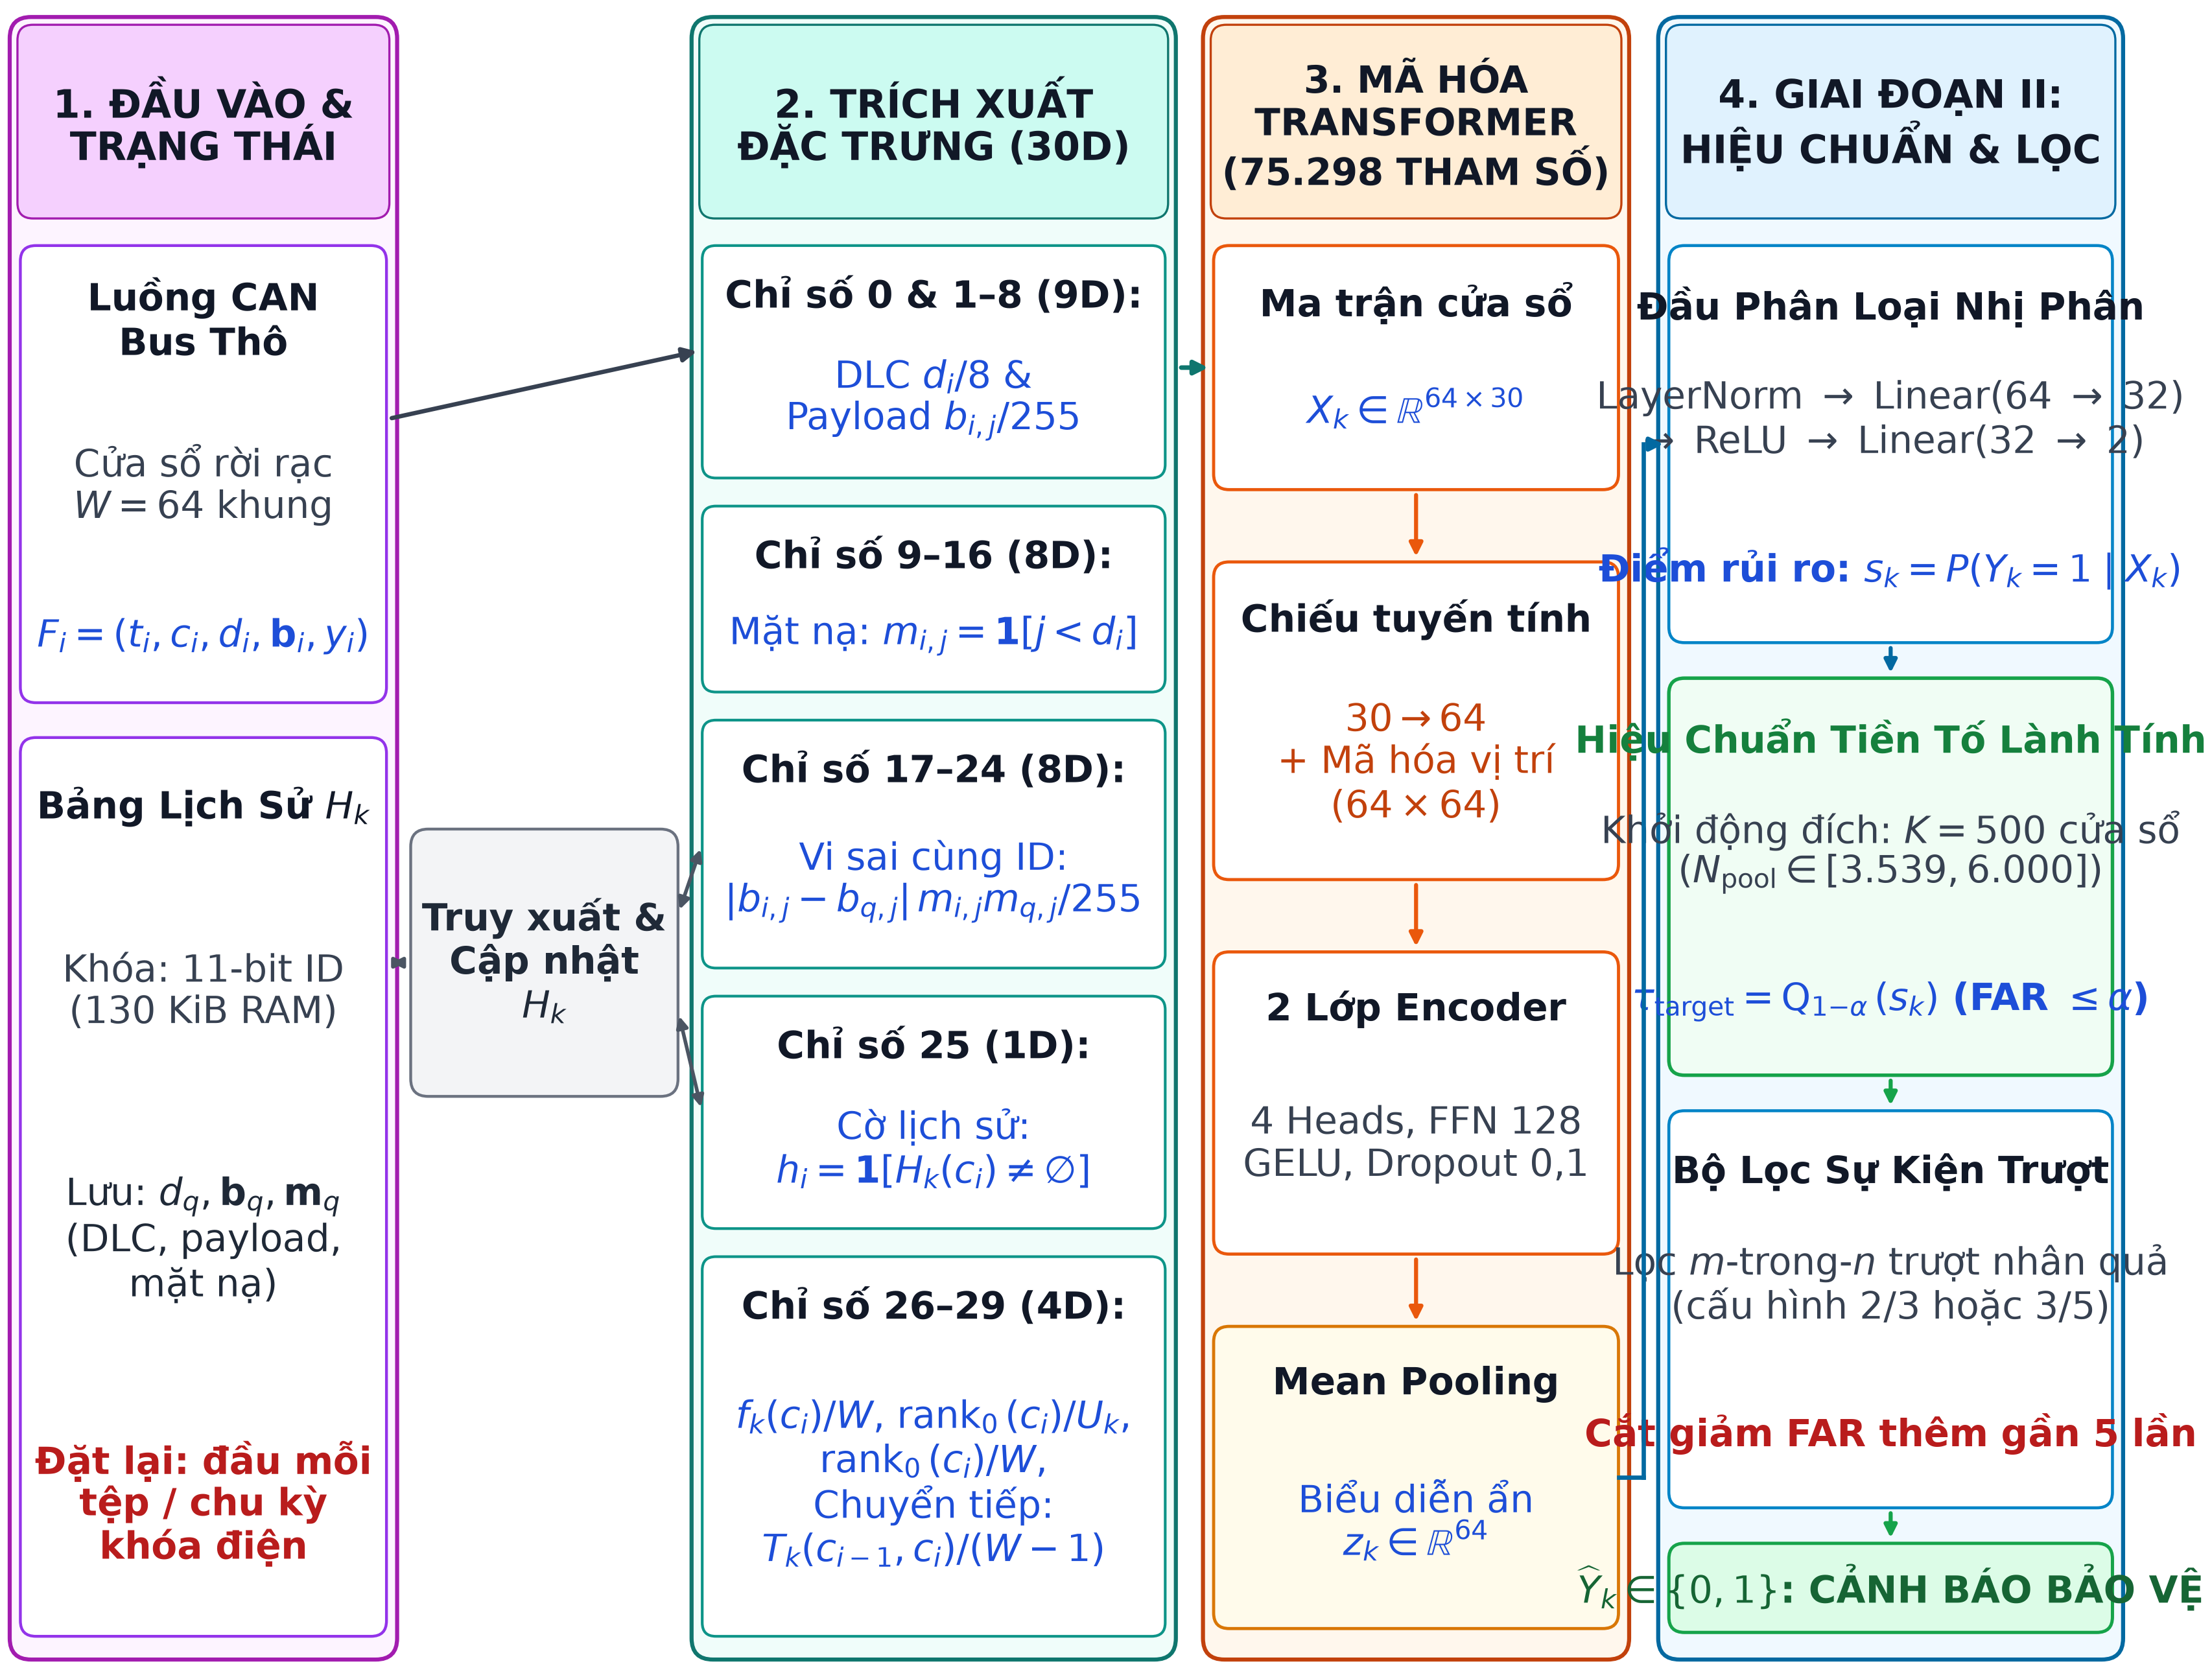
\includegraphics[width=0.98\textwidth]{figs/pipeline_architecture_30d.png}
\caption[Sơ đồ kiến trúc tổng thể khung phát hiện xâm nhập cấu trúc thích ứng ngưỡng]{Sơ đồ kiến trúc tổng thể khung phát hiện xâm nhập cấu trúc thích ứng ngưỡng hai giai đoạn: (1) Đầu vào luồng CAN thô ($W=64$) kết hợp cập nhật nhân quả bảng lịch sử $H_k$; (2) Trích xuất vector 30 chiều đặc trưng cấu trúc cấp khung tin; (3) Bộ mã hóa Transformer 2 tầng ($75.298$ tham số) kết hợp gộp trung bình tạo biểu diễn ẩn cửa sổ $z_k \in \mathbb{R}^{64}$; (4) Giai đoạn II: Đầu phân loại nhị phân, hiệu chuẩn phân vị tiền tố lành tính $K=500$ ($\tau_{\text{target}}$) và bộ lọc sự kiện trượt $m$-trong-$n$ phát cảnh báo $\widehat{Y}_k$.}\label{fig:architecture-30d}
\end{figure}

Các siêu tham số huấn luyện và ngân sách báo động giả chi tiết của thực nghiệm được trình bày tại Mục~\ref{sec:comparison-protocol} (Bảng~\ref{tab:config}).\par\medskip

\section{Giai đoạn II: Hiệu chuẩn ngưỡng vận hành trên tiền tố lành tính và lọc sự kiện trượt}\label{sec:method-calibration}
Dưới tác động của dịch chuyển hiệp phương sai và dịch chuyển điểm số giữa các dòng xe (Mục~\ref{subsec:domain-shifts}), ngưỡng quyết định đóng băng từ nguồn $\tau_{\text{src}}$ thường bị lệch nghiêm trọng so với phân phối nền lành tính của phương tiện mới. Thay vì tinh chỉnh trọng số mạng nơ-ron --- vốn đòi hỏi dữ liệu tấn công có nhãn trên xe đích và tiềm ẩn nguy cơ quên tri thức nguồn --- Giai đoạn II giữ đóng băng hoàn toàn bộ mã hóa Transformer $f_\theta$ và chỉ thích ứng duy nhất một ngưỡng phân loại vô hướng $\tau_{\text{target}}$ dựa trên một đoạn tiền tố lưu lượng lành tính không nhãn thu thập trên xe đích.

\paragraph{Giao thức xác định tiền tố hợp lệ không rò rỉ:} Gọi $L_{\text{benign}}^{(j)}$ là số cửa sổ lành tính liên tiếp ở đầu bản ghi thứ $j$ trước khi xuất hiện cửa sổ tấn công đầu tiên. Với ngân sách khởi động trần $K \in \{200, 500, 1000\}$ cửa sổ mỗi bản ghi, độ dài tiền tố hợp lệ dùng cho hiệu chuẩn ngoại tuyến được chặn trên bởi:
\begin{equation}
K_{\text{valid}}^{(j)} = \min\left(K, \left\lfloor \frac{L_{\text{benign}}^{(j)}}{2} \right\rfloor\right).
\end{equation}
Ràng buộc $\lfloor L_{\text{benign}}^{(j)} / 2 \rfloor$ đóng vai trò chốt an toàn chống rò rỉ nhãn trong đánh giá ngoại tuyến, bảo đảm đoạn hiệu chuẩn hoàn toàn sạch tấn công đồng thời giữ lại ít nhất một nửa tiền tố lành tính cho tập kiểm thử hậu khởi động. Khi triển khai vật lý trên phương tiện thực tế, $K$ cửa sổ khởi động được thu thập trực tiếp trong pha bật khóa điện / nổ máy tĩnh trước khi xe vận hành.

\paragraph{Ước lượng phân vị gộp đa bản ghi:} Cho tập hợp $J$ bản ghi của cùng một phương tiện đích, hệ thống trích xuất tuần tự các điểm rủi ro vô hướng $s(X_k^{(j)}) = \operatorname{softmax}(f_\theta(X_k^{(j)}))_1$ trên toàn bộ các cửa sổ tiền tố $k \in \{0, \dots, K_{\text{valid}}^{(j)} - 1\}$ và gộp thành đa tập nền $\mathcal{S}_{\text{warm}}$ có tổng kích thước $N_{\text{pool}} = \sum_{j=1}^{J} K_{\text{valid}}^{(j)}$. Tại ngân sách báo động giả danh định $\alpha \in \{0{,}1\%, 0{,}5\%, 1{,}0\%, 2{,}0\%\}$, ngưỡng vận hành trên xe đích được xác định bằng phân vị thực nghiệm:
\begin{equation}
\tau_{\text{target}} = \operatorname{Quantile}_{1-\alpha}(\mathcal{S}_{\text{warm}}).
\end{equation}
Theo phân tích sai số phân vị mẫu hữu hạn (Mục~\ref{subsec:theory-probing-dkw}), để phân vị đuôi tại mức $\alpha$ có ý nghĩa thống kê và không suy biến về giá trị cực đại, cỡ mẫu nền cần thỏa mãn điều kiện $N_{\text{pool}}\alpha \ge 1$. Cơ chế gộp đa phiên giúp thỏa mãn chặt chẽ điều kiện này ngay cả ở ngân sách khắt khe $\alpha = 0{,}1\%$; trong trường hợp triển khai trên một chuyến đi đơn lẻ chỉ có $K = 500$ cửa sổ ($K\alpha = 0{,}5 < 1$ tại $\alpha = 0{,}1\%$), hệ thống cần tích lũy nền qua nhiều chu kỳ khởi động hoặc vận hành ở ngân sách $\alpha \ge 0{,}5\%$ kết hợp bộ lọc sự kiện.

\paragraph{Bộ lọc sự kiện trượt $m$-trong-$n$:} Nhằm triệt tiêu các xung nhiễu báo động giả đơn lẻ trên đường truyền tốc độ cao (1.000--2.000 khung tin/giây), các quyết định nhị phân hậu khởi động ($k \ge K_{\text{valid}}^{(j)}$) đi qua bộ lọc trượt nhân quả:
\begin{equation}\label{eq:mofn-filter}
\hat{Y}_k^{(m/n)} = \mathbf{1}\!\left[\sum_{r = \max(K_{\text{valid}}^{(j)},\, k - n + 1)}^{k} \mathbf{1}\!\left[s(X_r) \ge \tau_{\text{target}}\right] \ge m\right],
\end{equation}
trong đó cảnh báo chính thức chỉ kích hoạt khi có ít nhất $m$ trong tối đa $n$ cửa sổ liên tiếp vượt ngưỡng ($m/n \in \{2/3, 3/5\}$). Về chi phí trực tuyến, bước hiệu chuẩn phân vị chỉ tốn $\mathcal{O}(N_{\text{pool}} \log N_{\text{pool}})$ một lần sau pha khởi động, còn bộ lọc trượt chỉ yêu cầu một bộ đệm vòng kích thước $n$. Toàn bộ quy trình được đặc tả hình thức trong Thuật toán~\ref{alg:benign-cal-mofn}.

\begin{algorithm}[htbp]
\caption{Hiệu chuẩn nền lành tính gộp đa bản ghi ($N_{\text{pool}}$) kết hợp bộ lọc sự kiện trượt $m$-trong-$n$}\label{alg:benign-cal-mofn}
{\small\linespread{1.05}\selectfont
\begin{algorithmic}[1]
\Require Bộ phân loại nguồn đóng băng $f_\theta$; tập hợp $J$ bản ghi của xe đích $\{\mathcal{C}^{(j)}\}_{j=1}^J$ với số cửa sổ lành tính đầu bản ghi $L_{\text{benign}}^{(j)}$; ngân sách khởi động trần mỗi bản ghi $K \in \{200, 500, 1000\}$; ngân sách báo động giả mục tiêu $\alpha \in \{0{,}1\%, 0{,}5\%, 1{,}0\%, 2{,}0\%\}$; tham số lọc trượt $(m, n)$ (mặc định $2/3, 3/5$).
\Ensure Ngưỡng vận hành xe đích $\tau_{\text{target}}$ và chuỗi cảnh báo sự kiện sau khởi động $\{\widehat{Y}_{k, (j)}^{(m/n)}\}$ cho từng bản ghi $j \in \{1, \ldots, J\}$.
\State \textbf{Giai đoạn 1 --- Thu thập điểm nền lành tính gộp đa bản ghi ($N_{\text{pool}}$):}
\State $\mathcal{S}_{\text{warm}} \leftarrow [\,]$ \Comment{Đa tập (multiset) tích lũy điểm số nền lành}
\For{$j = 1$ \textbf{to} $J$}
    \State $K_{\text{valid}}^{(j)} \leftarrow \min\big(K,\, \lfloor L_{\text{benign}}^{(j)} / 2 \rfloor\big)$ \Comment{Ngân sách tiền tố hợp lệ bảo đảm an toàn nhãn}
    \State Khởi tạo trạng thái lịch sử $H_0 \leftarrow \emptyset$ cho bản ghi $j$
    \For{$k = 0$ \textbf{to} $K_{\text{valid}}^{(j)} - 1$}
        \State $X_k^{(j)}, H_{k+1} \leftarrow \Phi(\mathcal{W}_k^{(j)}; H_k)$ \Comment{Trích xuất cấu trúc theo Thuật toán~\ref{alg:causal-30d}}
        \State $s(X_k^{(j)}) \leftarrow \operatorname{softmax}(f_\theta(X_k^{(j)}))_1$ \Comment{Điểm rủi ro từ bộ mã hóa nguồn}
        \State $\mathcal{S}_{\text{warm}} \leftarrow \mathcal{S}_{\text{warm}} \sqcup [s(X_k^{(j)})]$
    \EndFor
\EndFor
\State $N_{\text{pool}} \leftarrow |\mathcal{S}_{\text{warm}}| = \sum_{j=1}^J K_{\text{valid}}^{(j)}$ \Comment{Tổng số cửa sổ nền tích lũy}
\State \textbf{Giai đoạn 2 --- Hiệu chuẩn ngưỡng phân vị thực nghiệm trên xe đích:}
\State $\tau_{\text{target}} \leftarrow \operatorname{Quantile}_{1-\alpha}(\mathcal{S}_{\text{warm}})$ \Comment{Bảo đảm điều kiện cỡ mẫu đuôi $N_{\text{pool}}\alpha \ge 1$}
\State \textbf{Giai đoạn 3 --- Suy luận hậu khởi động và lọc sự kiện trượt $m$-trong-$n$ trên từng bản ghi:}
\For{$j = 1$ \textbf{to} $J$}
    \For{$k = K_{\text{valid}}^{(j)}$ \textbf{to} $M^{(j)} - 1$}
        \State $X_k^{(j)}, H_{k+1} \leftarrow \Phi(\mathcal{W}_k^{(j)}; H_k)$
        \State $s(X_k^{(j)}) \leftarrow \operatorname{softmax}(f_\theta(X_k^{(j)}))_1$
        \State $a_k \leftarrow \mathbf{1}\big[s(X_k^{(j)}) \ge \tau_{\text{target}}\big]$ \Comment{Quyết định nhị phân thô tại cửa sổ $k$}
        \State $j_0 \leftarrow \max(K_{\text{valid}}^{(j)},\, k - n + 1)$
        \State $\widehat{Y}_{k, (j)}^{(m/n)} \leftarrow \mathbf{1}\left[\sum_{r=j_0}^{k} a_r \ge m\right]$ \Comment{Phát cảnh báo khi có $\ge m$ trên $n$ cửa sổ vượt ngưỡng}
    \EndFor
\EndFor
\State \Return $\tau_{\text{target}}, \{\widehat{Y}_{k, (j)}^{(m/n)}\}$
\end{algorithmic}}
\end{algorithm}

\section{Tóm tắt chương}\label{sec:method-summary}
Chương~3 đã phát biểu hình thức bài toán phát hiện xâm nhập mạng CAN xuyên phương tiện và đặc tả trọn vẹn khung giải pháp đề xuất gồm hai giai đoạn cốt lõi: \textbf{Giai đoạn~I} xây dựng không gian biểu diễn cấu trúc 30 chiều độc lập định danh (cùng biến thể mở rộng động học thời gian 32 chiều cho luồng bus đồng hồ chuẩn) kết hợp bộ mã hóa Transformer 75.298 tham số; \textbf{Giai đoạn~II} bổ sung cơ chế hiệu chuẩn phân vị trên tiền tố lành tính không nhãn kết hợp bộ lọc sự kiện trượt $m$-trong-$n$ nhằm khôi phục điểm vận hành mà không huấn luyện lại mô hình. Chương~4 sẽ triển khai đánh giá thực nghiệm toàn diện khung đề xuất này cùng các phương pháp đối chứng trên nhiều dòng xe và bộ dữ liệu ngoại bộ độc lập.

\chapter{Thực nghiệm và đánh giá}\label{chap:results}

Chương này trình bày đánh giá thực nghiệm toàn diện cho khung phát hiện xâm nhập mạng nội xe hai giai đoạn đề xuất trên bộ đối chuẩn \textit{can-train-and-test} và ba bộ dữ liệu ngoại bộ độc lập. Nội dung chương được tổ chức thành ba phần nối tiếp:
\begin{itemize}
  \item \textbf{Mục~\ref{sec:exp-setup}:} Thiết lập dữ liệu, quy trình chia tách chống rò rỉ, các phương pháp đối chứng, siêu tham số huấn luyện và hệ thống độ đo đánh giá.
  \item \textbf{Mục~\ref{sec:exp-results}:} Phân tích kết quả thực nghiệm qua bốn nội dung trọng tâm: hiệu năng chuyển giao zero-shot Giai đoạn~I, khôi phục điểm vận hành Giai đoạn~II và đối chứng thuần xe đích, phân tích cắt bỏ cùng hiện tượng đan xen đặc trưng, và khả năng tổng quát hóa ngoại bộ kèm chi phí thực thi.
  \item \textbf{Mục~\ref{sec:exp-summary}:} Đúc kết các kết luận thực nghiệm chính của chương.
\end{itemize}

\section{Thiết lập thực nghiệm}\label{sec:exp-setup}

\subsection{Dữ liệu đối chuẩn và quy trình chia tách chống rò rỉ}\label{subsec:exp-data}

Thực nghiệm chính sử dụng bộ đối chuẩn \textit{can-train-and-test} (CTT)~\cite{lampe2024curated}
gồm 236 bản ghi thực tế thu thập trên bốn dòng xe vật lý (Chevrolet Impala, Chevrolet Traverse, Chevrolet Silverado và Subaru Forester), tổng cộng hơn 3,01 triệu cửa sổ rời rạc $W=64$. Các bản ghi được tổ chức thành bốn tập chuyển giao (Tập~1--4), mỗi tập bao gồm tập nguồn và bốn điều kiện kiểm thử A--D như thống kê tại Bảng~\ref{tab:ctt-split}.

\begin{table}[htbp]
  \centering
  \caption[Thống kê chia tách dữ liệu và phân bố họ tấn công trên bốn tập CTT]{Thống kê chia tách tập huấn luyện/validation nguồn, số lượng bản ghi kiểm thử và phân bố họ tấn công trên bốn tập \textit{can-train-and-test}}
  \label{tab:ctt-split}
  \footnotesize
  \begin{tabular}{@{}c c c c p{6.4cm}@{}}
    \toprule
    \textbf{Tập} & \textbf{Nguồn (Train/Val)} & \textbf{Test A/B/C/D} & \textbf{Hậu tố Val} & \textbf{Họ tấn công trong A--B / C--D} \\
    \midrule
    1 & 6/6 tệp & 8/8/12/12 & 2 & A--B: DoS, force-neutral, rpm, standstill; C--D: double, fuzzing, interval, speed, systematic, triple \\
    2 & 8/8 tệp & 12/12/8/8 & 2 & A--B: double, fuzzing, interval, speed, systematic, triple; C--D: DoS, force-neutral, rpm, standstill \\
    3 & 7/7 tệp & 10/10/14/14 & 4 & A--B: DoS, double, force-neutral, fuzzing, triple; C--D: interval, rpm, rpm-acc., speed, speed-acc., standstill, systematic \\
    4 & 9/9 tệp & 14/14/10/10 & 4 & A--B: interval, rpm, rpm-acc., speed, speed-acc., standstill, systematic; C--D: DoS, double, force-neutral, fuzzing, triple \\
    \bottomrule
  \end{tabular}
\end{table}

Để chống rò rỉ thông tin giữa huấn luyện và hiệu chuẩn ngưỡng nguồn, các bản ghi nguồn được tách theo hậu tố vòng ghi độc lập: tổng cộng 30 tệp huấn luyện nguồn (388.435 cửa sổ $W=64$) và 30 tệp validation nguồn (385.168 cửa sổ đầy đủ không cắt tỉa), hoàn toàn tách biệt với tập kiểm thử A--D. Quá trình huấn luyện sử dụng lấy mẫu hồ chứa (\textit{reservoir sampling}) với giới hạn tối đa 1.000 cửa sổ/lớp/tệp (dùng chung một hạt giống lấy mẫu cố định cho mọi mô hình), trong khi tập validation và kiểm thử A--D giữ nguyên phân bố lớp thực tế (tỷ lệ dương biến thiên từ 0,03\% đến 97,81\% tùy kịch bản). Do kiểm toán đầu vào ghi nhận 12.527 điểm đảo dấu thời gian ($\Delta t < 0$) trên 100/236 bản ghi CTT, ma trận đối sánh chính sử dụng nhánh thuần nội dung theo thứ tự khung tin (28D/30D) trên toàn bộ 236 tệp, và tách riêng nhánh động học thời gian (29D/32D) để kiểm chứng có đối chứng trên đúng 136 bản ghi đơn điệu nghiêm ngặt.

Đối với kiểm thử ngoại bộ (57 bản ghi hợp lệ từ ba bộ dữ liệu độc lập), nhãn DoS trên Automotive~v2~\cite{dupont2019automotive} được gán theo khoảng thời gian và chữ ký khung tin; CAN-MIRGU~\cite{rajapaksha2024canmirgu} đồng bộ nhãn trực tiếp từ nhật ký tấn công từng khung; CICIoV2024~\cite{neto2024ciciov2024} áp dụng chế độ thứ tự hàng không thời gian (loại trừ tệp tốc độ có bất thường cấu trúc nhãn); và OTIDS~\cite{lee2017otids} chưa đưa vào kết luận chính do cần xác minh thêm tính nhất quán nhãn sau chuyển đổi.

\subsection{Các phương pháp đối chứng và cấu hình huấn luyện}\label{subsec:exp-baselines}\label{sec:comparison-protocol}

Mọi mô hình nơ-ron đánh giá đều chạy lặp qua ba hạt giống khởi tạo (42, 43, 44) trên cùng tập mẫu nguồn và đơn vị cửa sổ $W=64$. Khung đề xuất được đặt lên bàn cân với ba nhóm đối chứng bao phủ đầy đủ các hướng tiếp cận hiện hành:

\begin{itemize}
  \item \textbf{Nhóm 1 -- Các mô hình IDS nền (đánh giá chuyển giao Giai đoạn~I):} \textit{Raw Transformer (28D)} dùng chung thân bộ mã hóa Transformer (75.170 tham số so với 75.298 của Structural) với đầu vào 11 bit CAN-ID, 1 chiều DLC, 8 byte payload và 8 bit mặt nạ hợp lệ; \textit{CANBERT+ adapted}~\cite{won2026canbertplus} (kiến trúc BERT 6 tầng, 54,25M tham số, tiền huấn luyện MLM 3 epoch và tinh chỉnh khung tin 3 epoch); \textit{CANLP-char-DNN adapted}~\cite{balasubramanian2025canlp} (TF-IDF ký tự + định danh qua mạng truyền thẳng 43.458 tham số); và \textit{CrySyS-AssocRules/W64}~\cite{koltai2026trust} (khai phá luật kết hợp không giám sát trên nền lành nguồn).
  \item \textbf{Nhóm 2 -- Các phương pháp thích ứng và triệt tiêu cấp biểu diễn:} \textit{MixStyle}~\cite{zhou2021mixstyle} (trộn thống kê kỳ vọng và độ lệch chuẩn cùng nhãn theo lô với $\alpha_{\text{mix}}=0{,}1, p=0{,}5$ lúc huấn luyện và đồng nhất khi suy luận); \textit{LOVO-cAdv}~\cite{ganin2016dann} (học đa nguồn giữ ngoài một xe trên 3 xe nguồn, tích hợp nhánh đối kháng có điều kiện định tuyến cứng theo nhãn lớp qua tầng đảo ngược gradient GRL, khảo sát cả biến thể 30D và biến thể lược bỏ payload tuyệt đối \textit{Relative+cAdv} 22D); cùng chuỗi hậu xử lý \textit{làm trắng hiệp phương sai nền lành tính} (ước lượng từ 2.000 cửa sổ lành đối chứng lọc trùng mã băm SHA-256) kết hợp triệt tiêu tuyến tính \textit{LEACE}~\cite{belrose2023leace}, \textit{INLP8}~\cite{ravfogel2020null} và điểm năng lượng Mahalanobis $E_{\text{white}}$~\cite{lee2018mahalanobis}.
  \item \textbf{Nhóm 3 -- Các bộ phát hiện mật độ thuần xe đích (Target-Only):} \textit{IsolationForest St60} (200 cây cô lập khớp trên vector tóm tắt trung bình + độ lệch chuẩn 60 chiều của tiền tố lành tính đích $N_{\text{pool}}$) và \textit{Split-Mahalanobis St60} (chia đôi tiền tố 250/250 cửa sổ mỗi tệp để ước lượng kỳ vọng, ma trận hiệp phương sai chính quy hóa co 0,1 và chọn ngưỡng phân vị ngoại mẫu) dùng cùng ngân sách quan sát $K=500$ và hoàn toàn không sử dụng dữ liệu xe nguồn.
\end{itemize}

Các siêu tham số huấn luyện mặc định của bộ mã hóa Transformer được tổng hợp tại Bảng~\ref{tab:hyperparams}. Trong Giai đoạn~I, ngưỡng quyết định nguồn $\tau_{\text{src}}$ được chọn tự động trên tập validation nguồn nhằm tối đa hóa Recall dưới ngân sách báo động giả $\text{FAR} \le 100/100.000$ cửa sổ lành tính (0,1\%), sau đó đóng băng hoàn toàn trước khi kiểm thử trên xe đích.

\begin{table}[htbp]
  \centering
  \caption[Siêu tham số huấn luyện và ngân sách báo động giả mặc định]{Các siêu tham số huấn luyện và ngân sách báo động giả mặc định của thực nghiệm}
  \label{tab:hyperparams}\label{tab:config}
  \footnotesize
  \begin{tabular}{@{}l l@{}}
    \toprule
    \textbf{Tham số} & \textbf{Giá trị} \\
    \midrule
    Cửa sổ chính / kiểm thử độ nhạy & 64 / 32 và 128 khung tin \\
    Kích thước ẩn / số tầng / số đầu chú ý & 64 / 2 / 4 \\
    Chiều mạng truyền thẳng / Dropout & 128 / 0,1 \\
    Bộ tối ưu / Tốc độ học / Weight decay & AdamW / $0{,}001$ / $10^{-4}$ \\
    Số epoch / Kích thước lô / Bộ điều lịch & 10 / 128 / Cosine theo epoch \\
    Hạt giống khởi tạo / Hạt giống lấy mẫu & 42, 43, 44 / 20261103 \\
    Giới hạn huấn luyện / Ngân sách FAR nguồn & 1.000 cửa sổ/lớp/tệp / $100/100.000$ cửa sổ lành \\
    \bottomrule
  \end{tabular}
\end{table}

\subsection{Hệ thống độ đo, môi trường tính toán và tính tái lập}\label{subsec:exp-metrics}

Dưới điều kiện mất cân bằng lớp nghiêm trọng trên bus CAN, nghiên cứu tách bạch hai nhóm độ đo: (1) \textbf{Chất lượng xếp hạng độc lập ngưỡng} đo bằng \textit{Average Precision (AP)}, phản ánh năng lực phân tách nội tại của biểu diễn trên đường cong Precision--Recall~\cite{saito2015pr}; và (2) \textbf{Hiệu năng tại điểm vận hành} gồm \textit{Recall}, \textit{Precision}, \textit{F1} và \textit{FAR} (tính trên 100.000 cửa sổ lành tính hoặc phần trăm \%). Mọi chỉ số tổng hợp được tính trung bình theo 3 hạt giống trong từng tập rồi gán trọng số ngang nhau giữa 4 tập, đồng thời kiểm chứng chéo theo trung bình khử lặp 3 xe đích vật lý phân biệt (do Subaru Forester lặp ở Tập~2 và Tập~3). Phép đo độ trễ suy luận thực hiện trên máy trạm AMD Ryzen~5 5600X (16~GB RAM) và GPU NVIDIA GeForce RTX~5060 (8~GB VRAM) với $\text{batch}=1$ (20 cửa sổ làm nóng + 900 cửa sổ đo lặp). Toàn bộ mã nguồn, mã băm toàn vẹn SHA-256 và hồ sơ kiểm chứng tái lập mở rộng được lưu trữ công khai cùng kho mã nguồn của nghiên cứu.

\section{Kết quả thực nghiệm và phân tích}\label{sec:exp-results}

\subsection{Hiệu năng chuyển giao zero-shot ở Giai đoạn I}\label{subsec:eval-stage1}

Bảng~\ref{tab:main-comparison} và Hình~\ref{fig:main-comparison} báo cáo kết quả đối sánh năm phương pháp ở cửa sổ $W=64$ dưới ngưỡng nguồn đóng băng qua bốn điều kiện A--D.

\begin{table}[htbp]
  \centering
  \caption[Kết quả đối sánh chính năm phương pháp tại $W=64$ dưới ngưỡng nguồn]{Kết quả đối sánh chính của năm phương pháp tại cửa sổ $W=64$ dưới ngưỡng đóng băng từ nguồn qua bốn điều kiện A--D (FAR tính trên 100.000 cửa sổ lành tính kèm phần trăm)}
  \label{tab:main-comparison}
  \footnotesize
  \begin{tabular}{@{}c l c c c c@{}}
    \toprule
    \textbf{ĐK} & \textbf{Phương pháp} & \textbf{Recall} & \textbf{FAR/100k (\%)} & \textbf{F1} & \textbf{AP} \\
    \midrule
    A & Raw Transformer & 0,6167 & 115,77 (0,12\%) & 0,7258 & 0,7312 \\
    A & Structural Transformer & 0,5886 & 81,67 (0,08\%) & 0,7072 & \textbf{0,7483} \\
    A & CANBERT+ adapted & 0,3843 & 79,27 (0,08\%) & 0,4576 & 0,5335 \\
    A & CANLP-char-DNN adapted & 0,1228 & 28,37 (0,03\%) & 0,1789 & 0,5482 \\
    A & CrySyS-AssocRules/W64$^\dagger$ & 0,0000 & 0,00 (0,00\%) & 0,0000 & 0,3338 \\
    \midrule
    B & Raw Transformer & 0,8541 & 65.301,41 (65,30\%) & 0,3000 & 0,3781 \\
    B & Structural Transformer & 0,7383 & 52.461,46 (52,46\%) & 0,2435 & \textbf{0,5554} \\
    B & CANBERT+ adapted & 0,6395 & 64.843,85 (64,84\%) & 0,0593 & 0,0970 \\
    B & CANLP-char-DNN adapted & 0,2854 & 29.695,88 (29,70\%) & 0,0329 & 0,0542 \\
    B & CrySyS-AssocRules/W64$^\dagger$ & 0,0000 & 0,00 (0,00\%) & 0,0000 & 0,0591 \\
    \midrule
    C & Raw Transformer & 0,2101 & 91,92 (0,09\%) & 0,2314 & 0,2661 \\
    C & Structural Transformer & 0,2230 & 75,82 (0,08\%) & \textbf{0,2600} & \textbf{0,2928} \\
    C & CANBERT+ adapted & 0,1037 & 62,54 (0,06\%) & 0,1461 & 0,2218 \\
    C & CANLP-char-DNN adapted & 0,0020 & 405,49 (0,41\%) & 0,0038 & 0,2373 \\
    C & CrySyS-AssocRules/W64$^\dagger$ & 0,0000 & 0,00 (0,00\%) & 0,0000 & 0,1732 \\
    \midrule
    D & Raw Transformer & 0,6614 & 67.982,89 (67,98\%) & 0,1213 & 0,1648 \\
    D & Structural Transformer & 0,6445 & 54.643,37 (54,64\%) & \textbf{0,2069} & \textbf{0,3357} \\
    D & CANBERT+ adapted & 0,5549 & 54.513,45 (54,51\%) & 0,0644 & 0,1311 \\
    D & CANLP-char-DNN adapted & 0,2491 & 25.452,19 (25,45\%) & 0,0119 & 0,0901 \\
    D & CrySyS-AssocRules/W64$^\dagger$ & 0,0000 & 0,00 (0,00\%) & 0,0000 & 0,0912 \\
    \bottomrule
    \multicolumn{6}{l}{\scriptsize $^\dagger$Ngưỡng nguồn suy biến lên trên điểm cực đại $1{,}0$ do không thỏa ngân sách validation ($R=0$, $\text{FAR}=0$).}
  \end{tabular}
\end{table}

\begin{figure}[htbp]
  \centering
  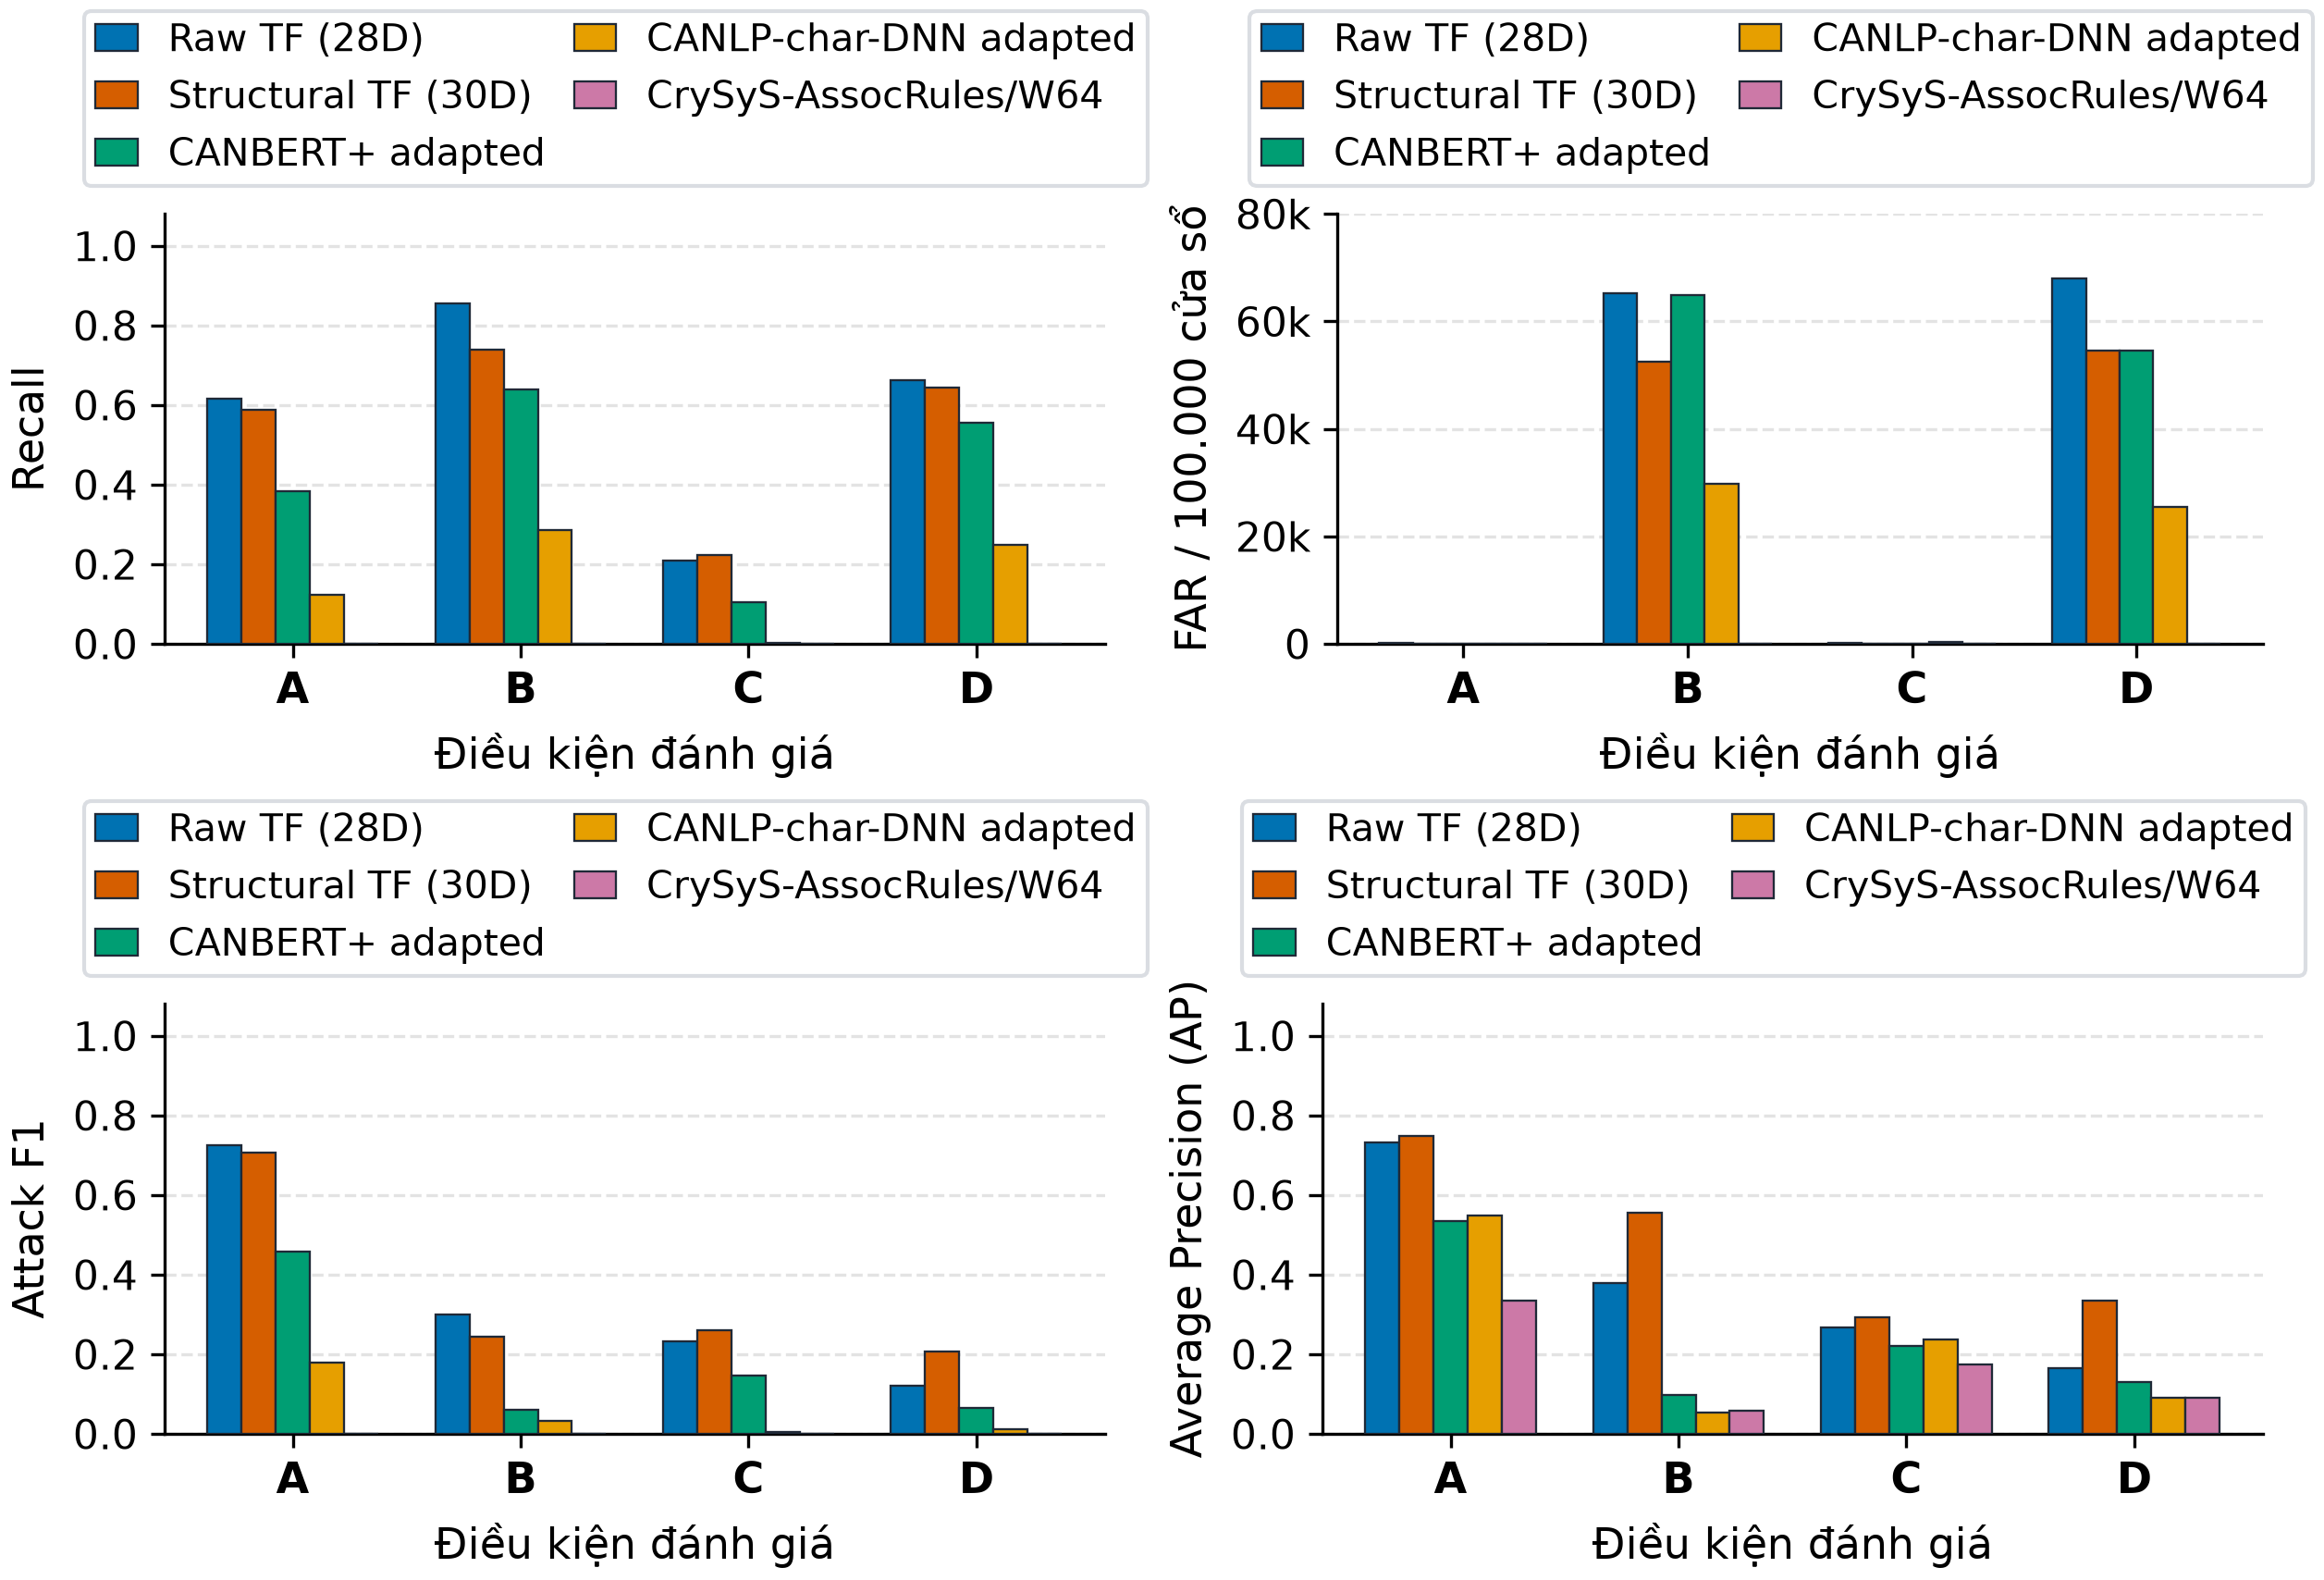
\includegraphics[width=\textwidth]{figs/main_comparison_w64.png}
  \caption[Kết quả đối sánh năm phương pháp ở cửa sổ $W=64$ qua bốn điều kiện A--D]{Kết quả đối sánh năm phương pháp ở cửa sổ $W=64$ qua bốn điều kiện A--D dưới ngưỡng nguồn (trọng số bốn tập ngang nhau).}
  \label{fig:main-comparison}
\end{figure}

Kết quả đối sánh chỉ ra sự phân kỳ rõ rệt giữa năng lực xếp hạng và điểm vận hành tĩnh. Ở Điều kiện~B (chuyển xe), toàn bộ các mô hình đều sụp đổ ngưỡng nguồn với FAR bùng nổ (Raw 65,30\%, CANBERT+ 64,84\%, Structural 52,46\%), trong khi Recall của Structural (0,7383) chưa vượt Raw (0,8541); điều này bác bỏ giả thuyết rằng loại bỏ CAN-ID thô tự động khôi phục vận hành zero-shot tại ngưỡng tĩnh. Trái lại, xét trên chất lượng xếp hạng độc lập ngưỡng, Structural Transformer vượt trội toàn diện khi nâng AP Điều kiện~B từ 0,3781 lên 0,5554 (+17,74 điểm phần trăm ghép cặp, gấp hơn 5 lần CANBERT+ 0,0970 và 10 lần CANLP 0,0542) và nhân đôi AP ở Điều kiện~D từ 0,1648 lên 0,3357 (+17,09 điểm phần trăm). Khi tính trung bình khử lặp 3 xe đích, xu hướng giữ nguyên tuyệt đối (Structural đạt AP 0,5510 ở B và 0,3404 ở D so với Raw 0,4281 và 0,1799).

Bóc tách cơ chế thất bại của các đối thủ nền cho thấy hai nguyên nhân chính: thứ nhất, CrySyS-AssocRules/W64 bị suy biến điểm vận hành trên toàn bộ 12 lượt chạy nguồn do tỷ lệ cửa sổ validation đạt điểm 1,0 vượt ngân sách 100/100k, và trên xe lạ 100\% cửa sổ đích nhận điểm cực đại (AP chỉ 0,0591 ở B); thứ hai, các mô hình cấp khung tin (CANBERT+, CANLP) chịu bất lợi quy nạp từ phép gộp cực đại $\max_{j=1}^{64} s_j$ làm khuếch đại xác suất báo động giả theo $1-(1-\epsilon)^{64} \approx 64\epsilon$. Ngay cả khi đổi sang quy tắc gộp trung bình (\textit{mean-pooling}) tối ưu hơn, AP Điều kiện~B của CANBERT+ (0,1636) và CANLP (0,1982) vẫn tụt hậu rất xa so với Structural (0,5554), xác nhận nút thắt bản chất nằm ở sự phụ thuộc từ vựng định danh xe nguồn.

\textbf{Tác động của động học thời gian trên 136 bản ghi đơn điệu (Bảng~\ref{tab:timed-vs-content}):} Để định lượng ảnh hưởng của quyết định loại bỏ biến thời gian trước 100 tệp CTT bị đảo dấu thời gian, thực nghiệm đối chứng nhánh thuần nội dung (28D/30D) và nhánh động học thời gian (29D/32D) trên đúng 136 bản ghi có dấu thời gian đơn điệu nghiêm ngặt.

\begin{table}[htbp]
  \centering
  \caption[Đối chứng nhánh thuần nội dung và động học thời gian trên 136 bản ghi đơn điệu]{Đối chứng nhánh thuần nội dung (28D/30D) và động học thời gian (29D/32D) trên 136 bản ghi CTT đơn điệu nghiêm ngặt (trung bình 4 tập $\times$ 3 hạt giống; trong ngoặc là trung bình khử lặp 3 xe đích)}
  \label{tab:timed-vs-content}
  \footnotesize
  \begin{tabular}{@{}l c c c c c c@{}}
    \toprule
    \textbf{Nhánh / Mô hình} & \textbf{Ngưỡng} & \textbf{ĐK} & \textbf{Recall (3-xe)} & \textbf{FAR (\%)} & \textbf{F1} & \textbf{AP (3-xe)} \\
    \midrule
    Content Raw (28D) & Nguồn & A & 0,7410 & 0,065 & 0,8390 & 0,8923 \\
    Timed Raw (29D) & Nguồn & A & 0,6371 & 0,108 & 0,7467 & 0,8399 \\
    Content Structural (30D) & Nguồn & A & 0,6100 & 0,088 & 0,7217 & 0,8182 \\
    Timed Structural (32D) & Nguồn & A & \textbf{0,8405} & 0,085 & \textbf{0,8996} & \textbf{0,9638} \\
    \midrule
    Content Raw (28D) & Nguồn & B & 0,9206 (0,8973) & 76,38 & 0,2624 & 0,5377 (0,6070) \\
    Timed Raw (29D) & Nguồn & B & 0,8249 (0,8086) & 65,88 & 0,2560 & 0,5788 (0,6501) \\
    Content Structural (30D) & Nguồn & B & 0,6479 (0,5808) & 41,16 & 0,2360 & 0,5786 (0,6123) \\
    Timed Structural (32D) & Nguồn & B & \textbf{0,8123} (0,8711) & \textbf{2,46} & \textbf{0,8274} & \textbf{0,9359} (0,9508) \\
    \midrule
    Content Structural (30D) & $K=500$, 1,0\% & B & 0,4264 (0,4689) & 2,24 & 0,5225 & 0,5857 (0,6185) \\
    Timed Structural (32D) & $K=500$, 1,0\% & B & \textbf{0,7460} (0,8035) & \textbf{0,63} & \textbf{0,8295} & \textbf{0,9451} (0,9575) \\
    Content Structural (30D) & $K=500$, 1,0\% & D & 0,2537 (0,3065) & 0,62 & 0,3213 & 0,3904 (0,4190) \\
    Timed Structural (32D) & $K=500$, 1,0\% & D & \textbf{0,4036} (0,4341) & \textbf{0,28} & \textbf{0,4742} & \textbf{0,7219} (0,6736) \\
    \bottomrule
  \end{tabular}
\end{table}

Trên luồng bus đồng hồ chuẩn, Timed Structural (32D) tạo bước nhảy vượt bậc ở Điều kiện~B khi nâng AP lên 0,9359 (0,9508 khử lặp 3 xe) và kéo FAR nguồn từ 41,16\% xuống 2,46\%, trong khi Timed Raw (29D) vẫn vỡ FAR ở mức 65,88\% — khẳng định động học thời gian chỉ phát huy tối đa khi ghép với biểu diễn cú pháp bất biến định danh. Tuy vậy, mức FAR 2,46\% vẫn vượt ngân sách nguồn 0,1\% tới 24,6 lần, chứng minh cả chế độ đồng hồ chuẩn lẫn chế độ thuần nội dung (cận dưới bảo thủ khi log nhiễu thời gian) đều bắt buộc cần khâu hiệu chuẩn ngưỡng ở Giai đoạn~II.

\subsection{Khôi phục điểm vận hành ở Giai đoạn II và đối chứng thuần xe đích}\label{subsec:eval-stage2}

Để hóa giải hiện tượng trôi dạt ngưỡng nguồn mà không huấn luyện lại mạng nơ-ron, Giai đoạn~II hiệu chuẩn phân vị trên tiền tố lành tính gộp $N_{\text{pool}} \in [3.539, 6.000]$ cửa sổ (ngân sách trần $K=500$ mỗi bản ghi) kết hợp bộ lọc sự kiện trượt $m$-trong-$n$. Hình~\ref{fig:calibration-recovery} và Bảng~\ref{tab:stage2-calibration} trình bày kết quả khôi phục điểm vận hành trên hai điều kiện chuyển xe B và D.

\begin{figure}[htbp]
  \centering
  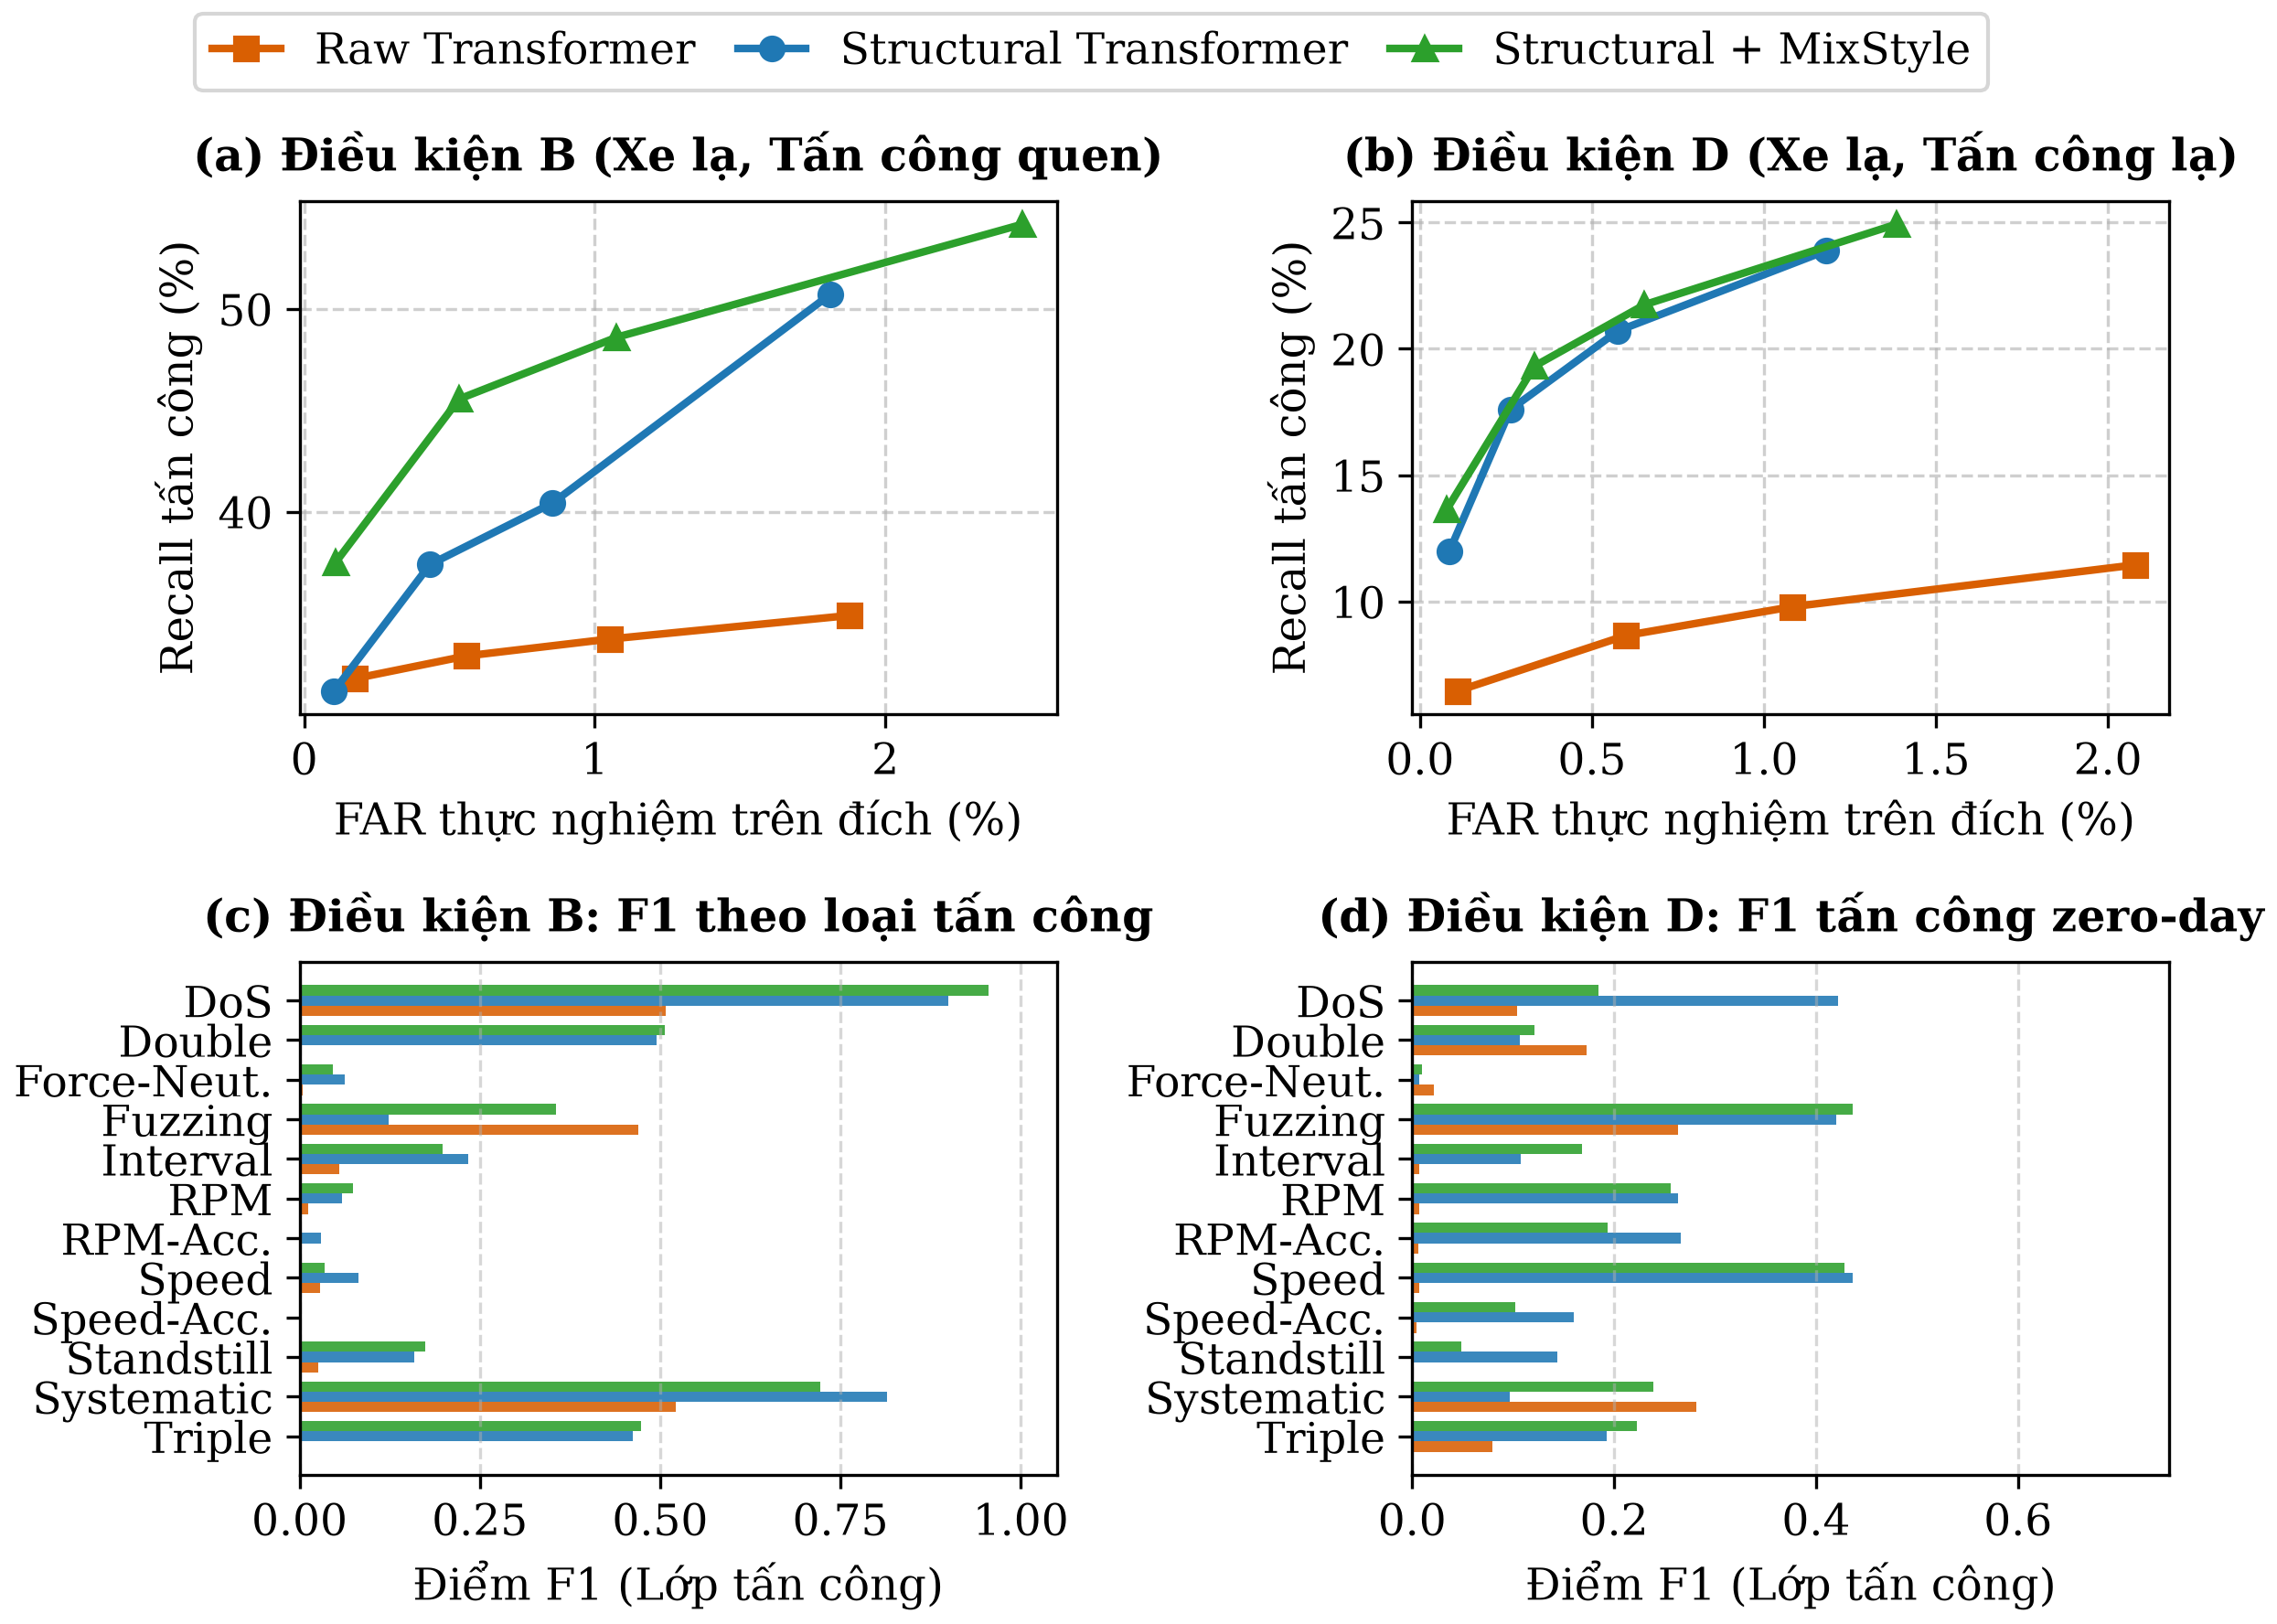
\includegraphics[width=\textwidth]{figs/calibration_recovery_comparison.png}
  \caption[Đánh giá khôi phục điểm vận hành qua hiệu chuẩn nền lành tính xe đích]{Đánh giá khôi phục điểm vận hành qua hiệu chuẩn nền lành tính xe đích: (a)--(b) Đường cong Recall theo FAR thực nghiệm tại $K=500$; (c)--(d) Điểm F1 theo từng họ tấn công ở Điều kiện~B và D tại $K=500, \alpha=1{,}0\%$.}
  \label{fig:calibration-recovery}
\end{figure}

\begin{table}[htbp]
  \centering
  \caption[Hiệu quả khôi phục điểm vận hành qua hiệu chuẩn tiền tố lành tính và lọc trượt]{Hiệu quả khôi phục điểm vận hành qua hiệu chuẩn tiền tố lành tính ($K=500$, $N_{\text{pool}} \in [3.539, 6.000]$, ngân sách $\alpha=1{,}0\%$) và bộ lọc sự kiện trượt $m$-trong-$n$}
  \label{tab:stage2-calibration}
  \footnotesize
  \begin{tabular}{@{}c l c c c c c c@{}}
    \toprule
    \textbf{ĐK} & \textbf{Phương pháp / Quy tắc lọc} & \textbf{FAR nguồn (\%)} & \textbf{Recall} & \textbf{FAR (\%)} & \textbf{F1} & \textbf{Precision} & \textbf{AP} \\
    \midrule
    B & CANBERT+ (Calib. max) & 64,84 & 0,2428 & 20,5601 & 0,1078 & -- & 0,0997 \\
    B & CANBERT+ (Calib. mean-pool) & 70,99 & 0,1183 & 1,8902 & 0,1562 & -- & 0,1665 \\
    B & CANLP-char-DNN (Calib. max) & 29,70 & 0,6578 & 68,2462 & 0,0794 & -- & 0,0564 \\
    B & CANLP-char-DNN (Calib. mean-pool) & 60,62 & 0,1402 & 1,7714 & 0,1835 & -- & 0,2011 \\
    B & Raw Transformer (1-of-1) & 65,30 & 0,3373 & 1,0509 & 0,3788 & -- & 0,3803 \\
    B & Structural Transformer (1-of-1) & 52,46 & 0,4042 & 0,8545 & 0,4748 & 0,6846 & 0,5607 \\
    B & Structural + MixStyle (1-of-1) & 64,54 & 0,4859 & 1,0752 & 0,5450 & 0,6603 & \textbf{0,5845} \\
    B & Structural + MixStyle (2-of-3) & 64,54 & 0,4911 & 0,2234 & 0,5903 & 0,8496 & -- \\
    B & Structural + MixStyle (3-of-5) & 64,54 & \textbf{0,4926} & \textbf{0,1387} & \textbf{0,5947} & \textbf{0,9131} & -- \\
    \midrule
    D & Raw Transformer (1-of-1) & 67,98 & 0,0979 & 1,0818 & 0,1195 & -- & 0,1692 \\
    D & Structural Transformer (1-of-1) & 54,64 & 0,2071 & 0,5750 & 0,2728 & -- & 0,3411 \\
    D & Structural + MixStyle (1-of-1) & 66,99 & \textbf{0,2175} & 0,6529 & \textbf{0,2852} & 0,4857 & \textbf{0,3702} \\
    D & Structural + MixStyle (2-of-3) & 66,99 & 0,1995 & 0,1160 & 0,2820 & 0,5738 & -- \\
    D & Structural + MixStyle (3-of-5) & 66,99 & 0,1919 & \textbf{0,0575} & 0,2747 & \textbf{0,6091} & -- \\
    \bottomrule
  \end{tabular}
\end{table}

Hiệu chuẩn Giai đoạn~II mang lại ba kết quả nổi bật:
\begin{enumerate}
  \item \textbf{Khôi phục kiểm soát FAR và cận sai số lý thuyết:} Tại $K=500, \alpha=1{,}0\%$ ở Điều kiện~B, Structural kéo FAR từ 52,46\% xuống 0,8545\% (Recall 40,42\%) và Structural+MixStyle đạt Recall 48,59\% với FAR trung bình $\le 1{,}0752\%$ (vượt xa mức 33,73\% của Raw và các đối thủ CANBERT+/CANLP kể cả sau khi đổi sang \textit{mean-pooling}). Khi thay đổi ngân sách khởi động trên Structural+MixStyle, Recall tăng ổn định từ 47,34\% ($K=200$, FAR 1,22\%) lên 51,41\% ($K=1000$, FAR 0,97\%). Theo bất đẳng thức DKW~\cite{massart1990dkw} ở độ tin cậy 95\% ($\delta=0{,}05$) với $N_{\text{pool}} \in [3.539, 6.000]$, sai số đồng đều tối đa bị chặn ở $\epsilon \le 2{,}28\%$--$1{,}75\%$ và sai số chuẩn nhị thức tại $\alpha=1{,}0\%$ đạt $0{,}17\%$--$0{,}13\%$. Trong thực nghiệm, FAR trung bình đạt $\le 1{,}08\%$, song vẫn phân tán giữa từng xe (thấp nhất 0,22\% ở Tập~3 và chạm 2,00\% ở Tập~4) do tính phi dừng và tự tương quan chuỗi của luồng CAN.
  \item \textbf{Hiệu quả bộ lọc sự kiện trượt $m$-trong-$n$:} Lọc trượt 2-trong-3 cắt FAR Điều kiện~B gần 5 lần xuống 0,2234\% (Precision 84,96\%, Recall 49,11\%), trong khi cấu hình 3-trong-5 tiếp tục hạ FAR xuống 0,1387\% ở B (Precision 91,31\%, F1 0,5947) và 0,0575\% ở D (Precision 60,91\%).
  \item \textbf{Phân rã họ tấn công và độ nhạy đầu độc khởi động:} Tại Điều kiện~B ($K=500, 1{,}0\%$), Structural+MixStyle đạt Recall 92,42\% trên DoS (F1 0,9438 so với Raw 0,5040) và 72,35\% trên Systematic (F1 0,7177), trong khi các cuộc tấn công biến thiên payload biên độ nhỏ như force-neutral (0,38\%) và speed (7,31\%) vẫn thách thức. Khi tiêm 1\%, 2\% và 5\% mẫu tấn công vào tiền tố khởi động $K=500$, Recall Điều kiện~B ($\alpha=1{,}0\%$) giảm lần lượt từ 48,59\% xuống 47,24\%, 44,95\% và 32,85\% (và giảm hơn một nửa ở $\alpha=0{,}1\%$ chỉ với 1\% nhiễm bẩn), khẳng định pha khởi động cần được thực hiện trong trạng thái sạch.
\end{enumerate}

\textbf{Đối chứng công bằng với các bộ phát hiện thuần xe đích (Target-Only, Bảng~\ref{tab:target-only}):} Một câu hỏi phương pháp luận quan trọng là khi đã thu thập tiền tố lành tính $K=500$ trên xe đích, liệu việc chuyển giao Transformer từ nguồn có thực sự cần thiết so với các thuật toán phát hiện mật độ không giám sát huấn luyện trực tiếp trên đích hay không.

\begin{table}[htbp]
  \centering
  \caption[Đối chứng giữa mô hình chuyển giao nguồn và bộ phát hiện thuần xe đích]{Đối chứng giữa mô hình chuyển giao nguồn (hiệu chuẩn $K=500$) và các bộ phát hiện thuần không giám sát chỉ dùng tiền tố đích $K=500$ (không dữ liệu nguồn)}
  \label{tab:target-only}
  \footnotesize
  \begin{tabular}{@{}l c c c c c c@{}}
    \toprule
    \textbf{Phương pháp} & \textbf{ĐK} & $\alpha$ & \textbf{Recall} & \textbf{FAR (\%)} & \textbf{F1} & \textbf{AP} \\
    \midrule
    Structural + MixStyle (Calib.) & B & 0,1\% & 0,3749 & \textbf{0,108} & 0,4955 & 0,5845 \\
    IsolationForest St60 (Target-Only) & B & 0,1\% & 0,3174 & 0,195 & 0,3888 & 0,5989 \\
    Split-Mahalanobis St60 (Target-Only) & B & 0,1\% & \textbf{0,6581} & 1,225 & \textbf{0,6829} & \textbf{0,7048} \\
    \midrule
    Structural + MixStyle (Calib.) & B & 1,0\% & 0,4859 & \textbf{1,075} & 0,5450 & 0,5845 \\
    IsolationForest St60 (Target-Only) & B & 1,0\% & 0,3889 & 2,708 & 0,3575 & 0,5989 \\
    Split-Mahalanobis St60 (Target-Only) & B & 1,0\% & \textbf{0,7007} & 4,999 & \textbf{0,5968} & \textbf{0,7048} \\
    \midrule
    Structural + MixStyle (Calib.) & D & 0,1\% & 0,1363 & \textbf{0,077} & 0,2026 & 0,3702 \\
    IsolationForest St60 (Target-Only) & D & 0,1\% & 0,2405 & 0,122 & 0,3238 & 0,5287 \\
    Split-Mahalanobis St60 (Target-Only) & D & 0,1\% & \textbf{0,6244} & 1,530 & \textbf{0,6344} & \textbf{0,7605} \\
    \midrule
    Structural + MixStyle (Calib.) & D & 1,0\% & 0,2175 & \textbf{0,653} & 0,2852 & 0,3702 \\
    IsolationForest St60 (Target-Only) & D & 1,0\% & 0,3931 & 1,713 & 0,4041 & 0,5287 \\
    Split-Mahalanobis St60 (Target-Only) & D & 1,0\% & \textbf{0,7193} & 7,564 & \textbf{0,5547} & \textbf{0,7605} \\
    \bottomrule
  \end{tabular}
\end{table}

Bảng~\ref{tab:target-only} làm sáng tỏ tính bổ trợ kiến trúc then chốt giữa biểu diễn cấu trúc 30 chiều và bộ mã hóa nguồn. Thứ nhất, ngay cả không cần nhãn nguồn, Split-Mahalanobis St60 đạt AP rất cao (0,7048 ở B và 0,7605 ở D), chứng tỏ bản thân không gian cấu trúc 30 chiều đã sở hữu tính phân tách hình học nội tại mạnh mẽ. Tuy nhiên, điểm yếu chí mạng của mô hình mật độ đa chiều là \textbf{vỡ hoàn toàn ngân sách FAR vùng đuôi}: Split-Mahalanobis trượt lên 1,225\%--4,999\% ở B và 1,530\%--7,564\% ở D (gấp 5--15 lần ngân sách danh định), còn IsolationForest trượt lên 1,713\%--2,708\% ở $\alpha=1{,}0\%$ đồng thời đòi hỏi nạp 200 cây cô lập vào SRAM khi khởi động. Nguyên nhân nằm ở lợi thế tham số: Split-Mahalanobis buộc phải ước lượng trực tiếp 1.890 tham số (60 kỳ vọng và 1.830 phần tử độc lập của ma trận hiệp phương sai $60\times 60$) trên tiền tố đích không dừng, trong khi Transformer nguồn đóng băng đóng vai trò \textbf{bộ nén rủi ro 1 chiều} (0 tham số biểu diễn cần ước lượng trên đích), chỉ hiệu chuẩn duy nhất 1 ngưỡng vô hướng $\tau_{\text{target}}$, nhờ đó kiểm soát chặt chẽ FAR vùng đuôi (0,077\%--0,108\% tại $\alpha=0{,}1\%$ và 0,653\%--1,075\% tại $\alpha=1{,}0\%$).

\subsection{Phân tích cắt bỏ, đan xen đặc trưng và đối chứng thích ứng cấp biểu diễn}\label{subsec:eval-ablation-probe}

\textbf{Phân tích cắt bỏ 10 biến thể biểu diễn và độ nhạy cửa sổ (Bảng~\ref{tab:ablation-compact}):} Để cô lập vai trò của từng nhóm đặc trưng trong không gian 30 chiều, thực nghiệm đánh giá 10 biến thể cắt bỏ trên cả bốn điều kiện A--D.

\begin{table}[htbp]
  \centering
  \caption[Phân tích cắt bỏ 10 biến thể biểu diễn tại $W=64$ qua bốn điều kiện A--D]{Phân tích cắt bỏ 10 biến thể biểu diễn tại kích thước cửa sổ $W=64$ dưới ngưỡng nguồn qua bốn điều kiện A--D}
  \label{tab:ablation-compact}
  \setlength{\tabcolsep}{3.5pt}
  \resizebox{\textwidth}{!}{%
  \begin{tabular}{@{}l c c c c c c c c c@{}}
    \toprule
    \textbf{Biến thể (Chiều)} & $\text{AP}_A$ & $\text{Rec}_B$ & $\text{FAR}_B$(\%) & $\text{F1}_B$ & $\text{AP}_B$ & $\text{AP}_C$ & $\text{Rec}_D$ & $\text{FAR}_D$(\%) & $\text{AP}_D$ \\
    \midrule
    Chỉ ID (11D) & \textbf{0,8492} & 0,8622 & 68,90 & 0,2573 & 0,3379 & 0,2736 & 0,6822 & 67,79 & 0,1914 \\
    Raw (28D) & 0,7312 & 0,8541 & 65,30 & 0,3000 & 0,3781 & 0,2661 & 0,6614 & 67,98 & 0,1648 \\
    Raw bỏ ID (17D) & 0,4139 & 0,6794 & 66,66 & 0,0875 & 0,2200 & 0,2222 & 0,6871 & 66,68 & 0,2175 \\
    Raw cộng cấu trúc (41D) & 0,7428 & 0,7604 & 53,23 & \textbf{0,3179} & 0,4842 & 0,2703 & 0,5783 & \textbf{52,90} & 0,2976 \\
    \textbf{Structural (30D, đề xuất)} & 0,7483 & 0,7383 & \textbf{52,46} & 0,2435 & 0,5554 & 0,2928 & 0,6445 & 54,64 & 0,3357 \\
    Structural bỏ vi sai $\Delta$ (21D) & 0,6789 & 0,8306 & 58,64 & 0,2861 & 0,4927 & 0,2720 & 0,6795 & 60,67 & 0,2745 \\
    Structural bỏ thống kê cục bộ (27D) & 0,6346 & 0,6870 & 65,30 & 0,0948 & 0,2894 & 0,2795 & 0,6925 & 66,40 & 0,3053 \\
    Structural bỏ payload tuyệt đối (22D) & 0,7644 & \textbf{0,9243} & 66,78 & 0,3160 & 0,4453 & \textbf{0,4730} & \textbf{0,7202} & 67,78 & 0,3138 \\
    Structural bỏ hạng/$W$ (29D) & 0,6837 & 0,7998 & 59,72 & 0,2425 & 0,5266 & 0,3420 & 0,6881 & 62,06 & 0,3446 \\
    Structural bỏ chuyển tiếp (29D) & 0,7044 & 0,7137 & 53,24 & 0,2220 & \textbf{0,5556} & 0,3210 & 0,6665 & 55,25 & \textbf{0,3679} \\
    \bottomrule
  \end{tabular}%
  }
\end{table}

Ba quy luật thiết kế nổi bật từ Bảng~\ref{tab:ablation-compact}: (1) xóa ID thô một cách cơ học (\textit{Raw bỏ ID}) làm $\text{AP}_B$ rơi từ 0,3781 xuống 0,2200; (2) \textit{thống kê cục bộ} và \textit{vi sai $\Delta\text{payload}$} là hai trụ cột quyết định khi loại bỏ chúng làm $\text{AP}_B$ tụt mạnh lần lượt về 0,2894 và 0,4927; và (3) bỏ payload tuyệt đối nâng mạnh phát hiện tấn công mới ở Điều kiện~C ($\text{AP}_C = 0{,}4730$ so với 0,2928) nhưng tăng FAR Điều kiện~B lên 66,78\%, nên không gian 30D đầy đủ giữ cân bằng tối ưu trên cả bốn điều kiện. Dưới kiểm chứng độ nhạy kích thước cửa sổ đẳng lượng (64.000 khung/tệp/lớp qua $W \in \{32, 64, 128\}$), Structural luôn vượt Raw về AP và xác lập điểm tối ưu tại $W=64$ ($\text{AP}_B = 0{,}5607$ sau hiệu chuẩn so với 0,4304 ở $W=32$ và 0,4903 ở $W=128$).

\textbf{Thăm dò tuyến tính và nguồn gốc hiện tượng đan xen đặc trưng (Bảng~\ref{tab:input-probes}):} Trên 12 cặp bộ mã hóa đóng băng (chia tách theo vòng ghi, cân bằng ô xe $\times$ nhãn với mức ngẫu nhiên 0,25 cho xe và 0,50 cho tấn công), thăm dò tuyến tính có đối chứng Hewitt--Liang~\cite{hewitt2019probes} ghi nhận khả năng giải mã tấn công tăng +12,50 điểm phần trăm từ 0,6419 (Raw) lên 0,7669 (Structural), nhưng độ chính xác giải mã danh tính xe chỉ giảm nhẹ từ 0,9925 xuống 0,9488 (các đối chứng hằng số, nhiễu ngẫu nhiên và hoán vị nhãn đều nằm quanh 0,25 và 0,50). Cô lập từng nhóm đặc trưng đầu vào (Bảng~\ref{tab:input-probes}) bóc tách chính xác nguồn gốc rò rỉ.

\begin{table}[htbp]
  \centering
  \caption[Khả năng giải mã tuyến tính nhãn xe và tấn công theo từng nhóm đặc trưng đầu vào]{Khả năng giải mã tuyến tính nhãn xe và nhãn tấn công từ từng nhóm đặc trưng đầu vào cô lập trên 8.440 cửa sổ cân bằng ($W=64$, 4.640 mẫu kiểm thử giữ ngoài)}
  \label{tab:input-probes}
  \footnotesize
  \begin{tabular}{@{}l c c c c@{}}
    \toprule
    \textbf{Nhóm đặc trưng đầu vào} & \textbf{Chiều/khung} & \textbf{Tổng chiều} & \textbf{Probe xe} & \textbf{Probe tấn công} \\
    \midrule
    Tất cả 30 đặc trưng (Structural) & 30 & 1.920 & 0,9804 & 0,7487 \\
    DLC, mặt nạ hợp lệ và cờ $h_i$ & 10 & 640 & 0,9670 & 0,6289 \\
    \quad -- Bóc tách riêng DLC và 8 mặt nạ & 9 & 576 & 0,9642 & 0,5946 \\
    \quad -- Bóc tách riêng cờ lịch sử $h_i$ & 1 & 64 & 0,2746 & 0,5662 \\
    Chỉ thống kê cục bộ & 3 & 192 & 0,7565 & 0,7269 \\
    Chỉ dữ liệu tải thô (payload) & 8 & 512 & 0,7621 & 0,5601 \\
    Chỉ vi sai dữ liệu tải ($\Delta$payload) & 8 & 512 & 0,6498 & 0,6420 \\
    Chỉ chuyển tiếp định danh & 1 & 64 & 0,4627 & 0,5013 \\
    Loại bỏ dữ liệu tải thô & 22 & 1.408 & 0,9565 & \textbf{0,7578} \\
    Loại bỏ vi sai dữ liệu tải (giữ cờ $h_i$) & 22 & 1.408 & 0,9884 & 0,7252 \\
    Loại bỏ thống kê cục bộ & 27 & 1.728 & 0,9541 & 0,6319 \\
    Loại bỏ chuyển tiếp định danh & 29 & 1.856 & 0,9778 & 0,7241 \\
    \bottomrule
  \end{tabular}
\end{table}

Ba kênh rò rỉ chính giải thích mức 94,88\%: nhóm 9 chiều hình thái khung (DLC và mặt nạ) giải mã xe tới 96,42\% do tỷ lệ khung 2/4/5/8 byte đặc thù từng hãng (giữ ổn định trong khoảng 0,9597--0,9670 qua mọi mức điều chuẩn $C \in [0{,}01, 10]$); nhóm thống kê cục bộ 3 chiều vừa giải mã xe 75,65\% vừa đạt probe tấn công cao nhất 72,69\%; và dải cảm biến payload đạt 76,21\%. Đây là bằng chứng trực tiếp của \textit{hiện tượng đan xen đặc trưng}: các kênh mang dấu ấn hãng xe cũng chính là tín hiệu nhạy bén nhất để phát hiện tấn công.

\textbf{Đối chứng với các cơ chế thích ứng và triệt tiêu cấp biểu diễn (Bảng~\ref{tab:adaptation-unified} và Hình~\ref{fig:erasure-overview}):} Để kiểm định liệu các kỹ thuật ép bất biến biểu diễn có thể thay thế Giai đoạn~II hay không, thực nghiệm đối chiếu đồng thời MixStyle, học đa nguồn đối kháng LOVO-cAdv và chuỗi làm trắng kết hợp LEACE/INLP8/$E_{\text{white}}$.

\begin{table}[htbp]
  \centering
  \caption[Đối chứng tổng hợp với ba nhóm kỹ thuật thích ứng và triệt tiêu cấp biểu diễn]{Đối chứng tổng hợp giữa khung đề xuất với ba nhóm phương pháp thích ứng và triệt tiêu cấp biểu diễn (Probe xe báo cáo cặp tuyến tính LR / phi tuyến MLP; dấu -- chỉ không áp dụng)}
  \label{tab:adaptation-unified}
  \footnotesize
  \begin{tabular}{@{}l c c c c c@{}}
    \toprule
    \textbf{Nhóm / Phương pháp} & \textbf{Recall} & \textbf{FAR (\%)} & \textbf{F1} & \textbf{AP} & \textbf{Probe xe (LR / MLP)} \\
    \midrule
    \multicolumn{6}{l}{\textit{Nhóm I: Điều chuẩn đơn nguồn (Điều kiện B, ngưỡng nguồn đóng băng)}} \\
    Structural Transformer & 0,7383 & 52,46 & 0,2435 & 0,5554 & 94,88\% / -- \\
    Structural + MixStyle ($\alpha_{\text{mix}}=0{,}1$) & 0,8194 & 64,54 & 0,2298 & 0,5815 & 95,27\% / -- \\
    \midrule
    \multicolumn{6}{l}{\textit{Nhóm II: Học đa nguồn đối kháng LOVO (4 xe giữ ngoài, ngưỡng validation 3 xe nguồn)}} \\
    Raw (LOVO) & 0,7885 & 69,84 & 0,2182 & 0,2196 & 99,74\% / 99,47\% \\
    Structural (LOVO) & 0,7211 & 37,02 & 0,4073 & 0,6020 & 94,49\% / 93,89\% \\
    Structural + cAdv & 0,7161 & 31,97 & 0,4254 & 0,5970 & 93,22\% / 92,36\% \\
    Relative + cAdv (22D) & 0,6579 & 29,72 & 0,4148 & 0,5764 & 94,74\% / 93,96\% \\
    \midrule
    \multicolumn{6}{l}{\textit{Nhóm III: Làm trắng và triệt tiêu tuyến tính trên LOVO đóng băng (lọc trùng SHA-256, $\alpha=1{,}0\%$)}} \\
    \textbf{Gốc / ngưỡng đích $\tau_{\text{target}}$} & \textbf{0,5180} & 1,009 & \textbf{0,6032} & 0,6042 & 94,18\% / 93,46\% \\
    Làm trắng nền lành + LR & 0,3876 & 1,036 & 0,4705 & 0,4852 & 64,29\% / 65,63\% \\
    Làm trắng + PCA8 + LR & 0,3765 & 1,100 & 0,4361 & 0,4603 & 54,08\% / 56,48\% \\
    Làm trắng + LEACE + LR & 0,3321 & 0,844 & 0,4065 & 0,4242 & 44,96\% / 57,19\% \\
    Làm trắng + INLP8 + LR & 0,3013 & 0,844 & 0,3750 & 0,3715 & \textbf{37,53\%} / \textbf{43,97\%} \\
    Năng lượng $E_{\text{white}}$ ($\alpha=0{,}1\%$) & 0,4606 & \textbf{0,297} & 0,5918 & \textbf{0,6172} & -- \\
    Năng lượng $E_{\text{white}}$ ($\alpha=1{,}0\%$) & 0,6008 & 3,831 & 0,5323 & \textbf{0,6172} & -- \\
    \bottomrule
  \end{tabular}
\end{table}

\begin{figure}[htbp]
  \centering
  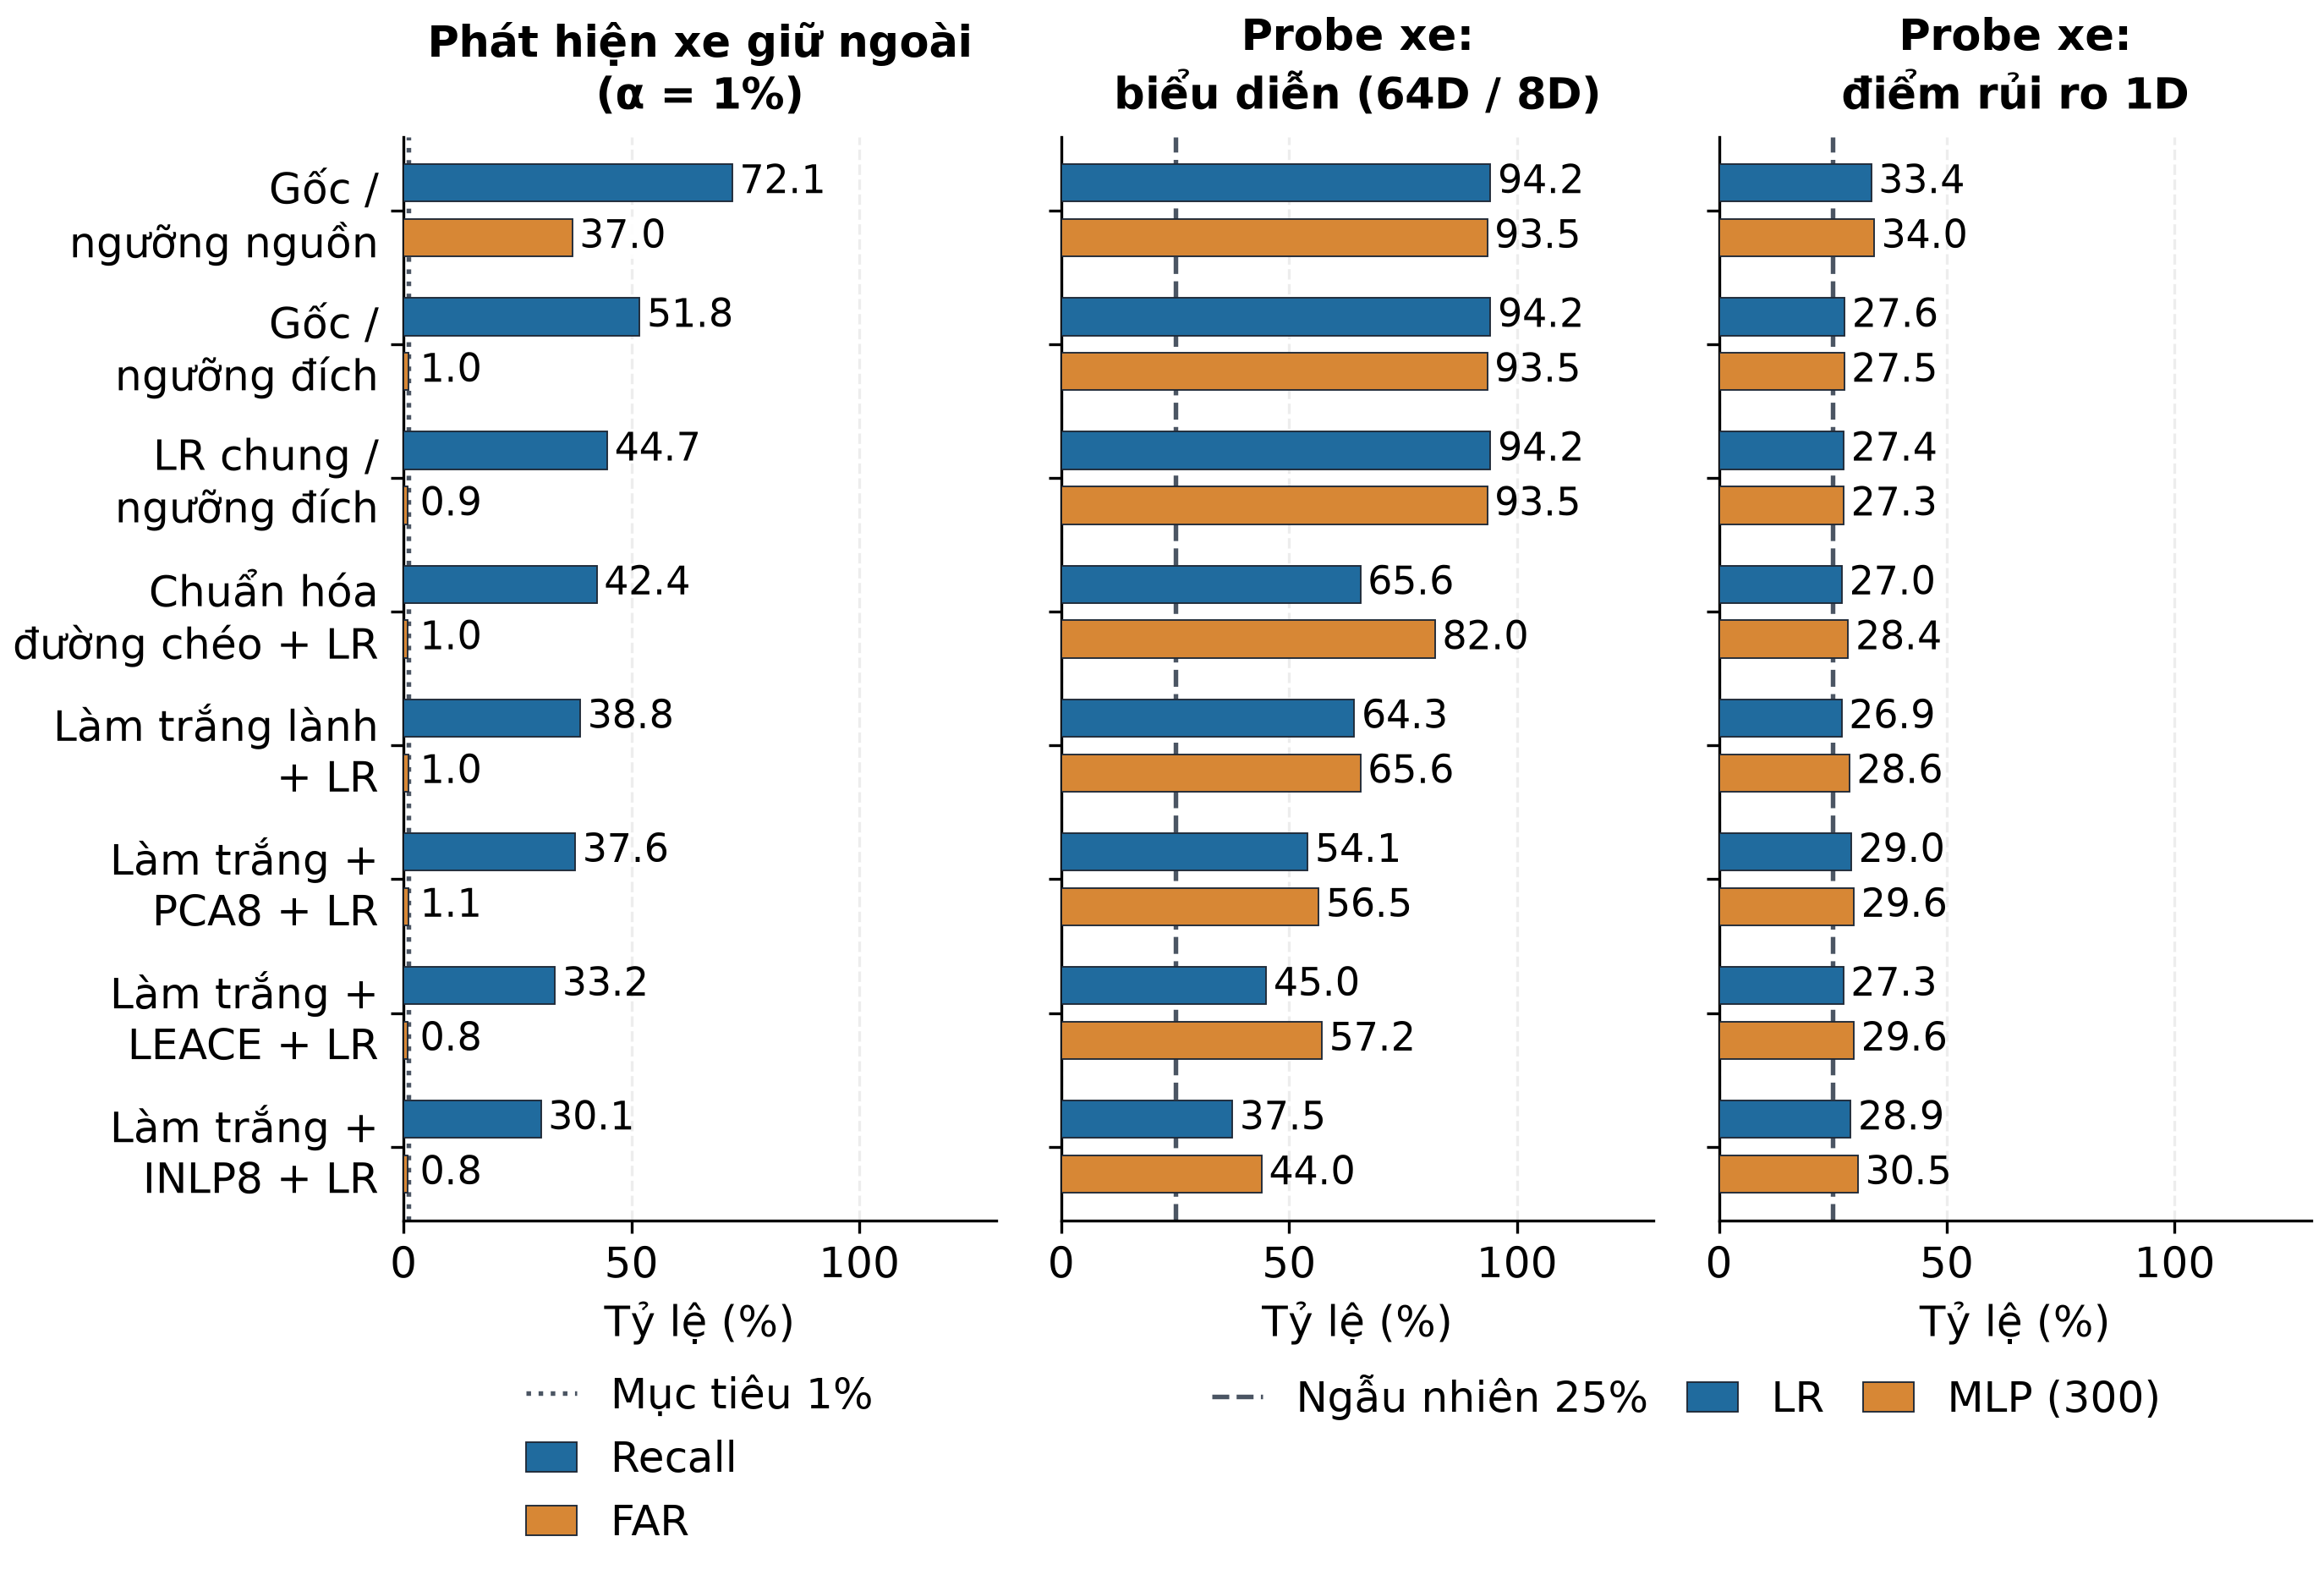
\includegraphics[width=\textwidth]{figs/benign_invariant_overview.png}
  \caption[Đối chiếu phát hiện tấn công và thăm dò xe sau làm trắng và triệt tiêu tuyến tính]{Đối chiếu đồng thời phát hiện tấn công ($\alpha=1{,}0\%$, lọc trùng mã băm SHA-256), thăm dò 4 xe trên biểu diễn đặc trưng (không gian 64D gốc hoặc chiếu 8D dư đối với PCA8 và INLP8) và thăm dò trên điểm rủi ro 1 chiều (mức ngẫu nhiên 25\%).}
  \label{fig:erasure-overview}
\end{figure}

Bảng~\ref{tab:adaptation-unified} và Hình~\ref{fig:erasure-overview} xác lập ba giới hạn cốt lõi của nhóm phương pháp ép bất biến cấp đặc trưng: (1) MixStyle nâng AP lên 0,5815 nhưng kéo FAR nguồn lên 64,54\% và không giảm rò rỉ xe (95,27\%), nên chỉ có tác dụng cải thiện thứ tự xếp hạng trước hiệu chuẩn ngưỡng; (2) học đa nguồn đối kháng LOVO-cAdv nâng AP lên 0,6020 và hạ FAR nguồn xuống 29,72\%--31,97\%, song vẫn quá cao để vận hành thực tế (riêng Forester chạm FAR 79,91\%) và giữ probe xe ở mức 93,22\%--94,74\%; (3) triệt tiêu tuyến tính LEACE/INLP8 giảm được probe tuyến tính 64D xuống 44,96\%/37,53\%, nhưng làm Recall sụp mạnh từ 51,80\% xuống 33,21\%/30,13\% trong khi bộ giải mã phi tuyến MLP 1.500 vòng vẫn trích xuất được 57,17\%/42,01\% danh tính xe (còn điểm năng lượng $E_{\text{white}}$ dù đạt AP cao nhất 0,6172 vẫn bị trượt FAR lên 3,831\% ở $\alpha=1{,}0\%$). Điều này chứng minh chiến lược tách bạch hai giai đoạn — bảo toàn biểu diễn giàu thông tin ở Giai đoạn~I và hiệu chuẩn ngưỡng 1 chiều ở Giai đoạn~II — là lựa chọn tối ưu.

\subsection{Tổng quát hóa ngoại bộ và hiệu năng thực thi}\label{subsec:eval-external-runtime}\label{sec:runtime}

\textbf{Đánh giá trên 57 bản ghi ngoại bộ trước và sau hiệu chuẩn (Bảng~\ref{tab:external-unified}):} Sử dụng mô hình neo huấn luyện từ Tập~1 (xe nguồn Chevrolet Impala, 3 hạt giống) đánh giá trực tiếp trên Automotive~v2, CICIoV2024 và CAN-MIRGU ở cả trạng thái ngưỡng nguồn lẫn sau hiệu chuẩn nền lành tính ($K=500, \alpha=0{,}1\%$).

\begin{table}[htbp]
  \centering
  \caption[Đánh giá tổng quát hóa trên 57 bản ghi ngoại bộ trước và sau hiệu chuẩn]{Đánh giá tổng quát hóa trên 57 bản ghi ngoại bộ trước và sau hiệu chuẩn nền lành tính Giai đoạn~II ($K=500, \alpha=0{,}1\%$, trung bình 3 hạt giống)}
  \label{tab:external-unified}
  \footnotesize
  \begin{tabular}{@{}l l c c c c@{}}
    \toprule
    & & \multicolumn{2}{c}{\textbf{Ngưỡng nguồn}} & \multicolumn{2}{c}{\textbf{Sau hiệu chuẩn ($K=500, 0{,}1\%$)}} \\
    \cmidrule(lr){3-4} \cmidrule(lr){5-6}
    \textbf{Bộ dữ liệu / Kịch bản} & \textbf{Mô hình} & \textbf{Recall} & \textbf{FAR (\%)} & \textbf{Recall} & \textbf{FAR (\%)} \\
    \midrule
    Renault Clio (DoS) & Raw TF & 0,9995 & 33,10 & -- & 0,051$^*$ \\
    Renault Clio (DoS) & Structural TF & 0,9984 & 0,19 & \textbf{0,9984} & \textbf{0,000} \\
    Opel Astra (DoS) & Structural TF & 1,0000 & 31,53 & 1,0000 & $3,271 \pm 0{,}266$ \\
    Opel Astra (DoS) & Structural + MixStyle & 1,0000 & 33,43 & \textbf{1,0000} & $\mathbf{0{,}167 \pm 0{,}079}$ \\
    CICIoV2024 & Structural TF & 1,0000 & 100,00 & $0,3336 \pm 0{,}5242$ & 0,047 \\
    CICIoV2024 & Structural + MixStyle & 1,0000 & 100,00 & $0{,}0001 \pm 0{,}0002^\dagger$ & 0,086 \\
    CAN-MIRGU (tấn công) & Structural TF & 0,0546 & 2,70 & 0,0065 & 0,087 \\
    CAN-MIRGU (tấn công) & Structural + MixStyle & 0,0486 & 1,83 & 0,0072$^\ddagger$ & 0,094 \\
    \bottomrule
    \multicolumn{6}{l}{\scriptsize $^*$FAR trên tệp lành tính Renault Clio. $^\dagger$Tại $\alpha=1{,}0\%$ đạt $0{,}3229 \pm 0{,}5593$. $^\ddagger$Tại $\alpha=1{,}0\%$ đạt 0,0275--0,0308 (FAR lành 1,135\%--1,236\%).}
  \end{tabular}
\end{table}

Trên các kịch bản DoS thực tế, khung hai giai đoạn hoạt động xuất sắc: Renault Clio triệt tiêu hoàn toàn FAR về 0,000\% (giữ Recall 99,84\%), còn Opel Astra (Structural+MixStyle) kéo FAR từ 33,43\% xuống 0,167\% với Recall 100\%. Ngược lại, kiểm toán sâu bóc tách hai cơ chế thất bại đặc thù trên hai bộ còn lại:
\begin{itemize}
  \item \textbf{Độ lệch miền mô phỏng trên CICIoV2024:} Toàn bộ tệp lành tính có độ dài cố định $\text{DLC}=8$ kèm mật độ ID cao ($U_k = 33{,}35 \pm 3{,}30$ so với 26,75--28,34 của CTT) kích hoạt FAR 100\% tại ngưỡng nguồn; ngược lại, các tệp tấn công không ghép kênh lưu lượng nền làm $U_k$ sụp về $1{,}00 \pm 0{,}00$ tạo phân tách nhân tạo ($\text{AP} = 0{,}9172 \pm 0{,}0711$) nhưng gây phương sai rất lớn giữa các hạt giống sau hiệu chuẩn.
  \item \textbf{Tấn công ngụy trang giữ nguyên chu kỳ trên CAN-MIRGU:} Các kịch bản mạo danh phát đúng nhịp ECU gốc với biến thiên byte rất nhỏ cùng các pha đình chỉ không chèn khung tin khiến biên độ đặc trưng không vượt ngưỡng nhạy cảm, giữ Recall ở mức 0,65\%--3,08\% sau hiệu chuẩn.
\end{itemize}

\textbf{Phân rã độ trễ và độ phức tạp tĩnh (Bảng~\ref{tab:runtime-breakdown}):} Bảng~\ref{tab:runtime-breakdown} cô lập chi phí xử lý ba thành phần theo từng cửa sổ $W=64$ ($\text{batch}=1$, trung vị trên 900 cửa sổ kiểm chuẩn). Do MixStyle chuyển về ánh xạ đồng nhất khi suy luận, chi phí suy luận của Structural+MixStyle hoàn toàn tương đương Structural.

\begin{table}[htbp]
  \centering
  \caption[Phân rã độ trễ xử lý ba thành phần theo cửa sổ $W=64$ trên CPU và GPU]{Phân rã độ trễ xử lý ba thành phần theo từng cửa sổ $W=64$ trên CPU và GPU ($N=900, \text{batch}=1$, đơn vị ms)}
  \label{tab:runtime-breakdown}
  \footnotesize
  \begin{tabular}{@{}l c c c c@{}}
    \toprule
    \textbf{Thiết bị} & \textbf{Đọc CSV (Median)} & \textbf{Trích xuất kép 28D+30D} & \textbf{Suy luận Structural} & \textbf{Tổng E2E (Median / P95)} \\
    \midrule
    CPU & 1,083 & 3,036 & \textbf{0,731} & 4,830 / 6,231 \\
    CUDA & 0,932 & 2,285 & 1,150 & 4,402 / 5,291 \\
    \bottomrule
  \end{tabular}
\end{table}

Thời gian suy luận thuần của Structural Transformer trên CPU chỉ tốn 0,731~ms (nhanh hơn CUDA 1,150~ms ở $\text{batch}=1$ do tránh phụ phí truyền dữ liệu); cộng thêm 32--64~ms gom đủ $W=64$ khung tin trên bus 500~kbps, tổng độ trễ phát hiện vào khoảng 37--70~ms. Về tài nguyên tĩnh, Structural Transformer chỉ có 75.298 tham số (+128 tham số hay +0,17\% so với Raw; nhẹ hơn CANBERT+ 54,25M tham số tới 720 lần) và 5,37M MACs/cửa sổ (nhẹ hơn CANBERT+ 5.075 lần). Bảng trạng thái lịch sử $H_k$ cho không gian 11-bit tiêu tốn 130,00~KiB ở bản tham chiếu Python và nén gọn xuống $\approx 20{,}48$~KiB khi hiện thực hóa kiểu \texttt{uint8\_t} trong C/C++, hoàn toàn nằm gọn trong SRAM của vi điều khiển ô tô.

\section{Tóm tắt chương}\label{sec:exp-summary}

Chương này đã kiểm chứng thực nghiệm toàn diện khung phát hiện xâm nhập cấu trúc hai giai đoạn qua ba kết luận cốt lõi: (1) ở Giai đoạn~I, biểu diễn cấu trúc 30 chiều nâng vượt trội chất lượng xếp hạng độc lập ngưỡng ($\text{AP}_B$ từ 0,3781 lên 0,5554; đạt 0,9359 khi mở rộng động học thời gian 32D trên 136 bản ghi đơn điệu), nhưng ngưỡng tĩnh nguồn bị sụp đổ do hiện tượng đan xen đặc trưng (giải mã xe 94,88\%, bắt nguồn từ nhóm DLC--mặt nạ đạt 96,42\%); (2) ở Giai đoạn~II, hiệu chuẩn tiền tố lành tính kết hợp lọc trượt $m$-trong-$n$ khôi phục vận hành thực tế (FAR giảm về $\le 1{,}08\%$ và 0,1387\%--0,2234\% sau lọc trượt), vượt trội cả các kỹ thuật ép bất biến cấp đặc trưng (MixStyle, LOVO-cAdv, LEACE/INLP8) lẫn mô hình mật độ thuần xe đích về độ ổn định FAR vùng đuôi nhờ chỉ hiệu chuẩn 1 ngưỡng vô hướng thay vì 1.890 tham số; và (3) kiểm thử 57 bản ghi ngoại bộ cùng phân rã độ trễ (0,731~ms suy luận CPU, 75k tham số, $\approx 20{,}48$~KiB bộ nhớ nhúng) xác lập rõ năng lực ứng dụng cũng như ranh giới thất bại của hệ thống.

\chap{Kết luận và hướng phát triển}\label{chap:conclusion}
\sect{Các đóng góp chính}
Mục tiêu cốt lõi của khóa luận là xây dựng và kiểm chứng một khung phát hiện xâm nhập dựa trên biểu diễn cấu trúc có khả năng chuyển giao xuyên phương tiện mà không cần dữ liệu tấn công có nhãn trên xe đích. Quá trình thiết kế, thực nghiệm đối chứng và chẩn đoán có kiểm soát đã hoàn thành mục tiêu đề ra thông qua bốn kết quả chính:

Thứ nhất, khóa luận thiết kế và kiểm chứng không gian biểu diễn cấu trúc 30 chiều độc lập định danh kết hợp bộ mã hóa Transformer gọn nhẹ (75.298 tham số). Trên bộ đối chuẩn can-train-and-test ở chế độ thuần nội dung, dù ngưỡng tĩnh đóng băng từ nguồn chưa tự động nâng độ nhạy (Recall điều kiện B đạt $73{,}83\%$ so với $85{,}41\%$ của biểu diễn thô) và chịu trôi dạt báo động giả nghiêm trọng ($\text{FAR} = 52{,}46\%$), biểu diễn cấu trúc nâng vượt trội chất lượng xếp hạng độc lập ngưỡng với AP tăng từ $0{,}3781$ lên $0{,}5554$ ($+17{,}74$ điểm phần trăm ghép cặp, vượt xa CANBERT+ ở mức $0{,}0970$ và CANLP ở mức $0{,}0542$). Khi dấu thời gian đơn điệu sạch khả dụng (136 bản ghi), biến thể mở rộng 32 chiều tiếp tục nâng AP điều kiện B lên $0{,}9359$ và kéo FAR nguồn xuống $2{,}46\%$ (dù vẫn cao gấp 24,6 lần ngân sách nguồn $0{,}1\%$). Các phép cắt bỏ khẳng định nhóm thống kê cục bộ và vi sai dữ liệu tải ($\Delta\text{payload}$) là hai trụ cột quyết định năng lực phân tách tại kích thước cửa sổ tối ưu $W = 64$.

Thứ hai, khóa luận làm sáng tỏ nguồn gốc của sự sụp đổ ngưỡng tĩnh thông qua chẩn đoán hiện tượng đan xen đặc trưng. Phép thăm dò tuyến tính có đối chứng Hewitt--Liang chứng minh rằng dù đã loại bỏ hoàn toàn 11 bit CAN-ID thô, dấu ấn hãng xe vẫn tồn lưu sâu sắc trong không gian ẩn (độ chính xác giải mã xe đạt $94{,}88\%$ so với mức ngẫu nhiên $25{,}00\%$), bắt nguồn chủ yếu từ nhóm cú pháp độ dài DLC và mặt nạ byte ($96{,}42\%$) cùng mật độ bus cục bộ ($75{,}65\%$) --- cũng chính là những tín hiệu cốt lõi để phân tách tấn công. Thực nghiệm mở rộng cho thấy các kỹ thuật điều chuẩn và triệt tiêu cấp đặc trưng (MixStyle, học đa nguồn đối kháng LOVO-cAdv, làm trắng kết hợp LEACE/INLP8) giúp cải thiện biên phân tách (AP đạt $0{,}5815\text{--}0{,}6172$), nhưng không thể xóa bỏ hoàn toàn ranh giới miền (FAR nguồn vẫn ở mức $29{,}72\%\text{--}64{,}54\%$ và thăm dò phi tuyến MLP sau triệt tiêu tuyến tính vẫn giải mã xe ở mức $42{,}01\%\text{--}57{,}17\%$).

Thứ ba, khóa luận xây dựng cơ chế hiệu chuẩn phân vị trên tiền tố lành tính không nhãn kết hợp bộ lọc sự kiện trượt $m$-trong-$n$ nhằm khôi phục điểm vận hành thực tế mà không tinh chỉnh mạng nơ-ron. Tại ngân sách danh định $\alpha = 1{,}0\%$ với tiền tố gộp ($N_{\text{pool}} \in [3.539, 6.000]$ cửa sổ), hệ thống kiểm soát tốt tỷ lệ báo động giả trung bình ($\le 1{,}08\%$, dao động từ $0{,}22\%$ ở Tập 3 đến $2{,}00\%$ ở Tập 4) và khôi phục Recall điều kiện B đạt $40{,}42\%\text{--}48{,}59\%$ (vượt mức $33{,}73\%$ của biểu diễn thô); bổ sung lọc trượt 2-trong-3 tiếp tục hạ FAR trung bình xuống $0{,}22\%$ với Precision đạt $84{,}96\%$. Đối chứng công bằng với các bộ phát hiện mật độ thuần xe đích cho thấy lợi thế tham số then chốt: trong khi mô hình Split-Mahalanobis đạt AP cao ($0{,}7048\text{--}0{,}7605$) nhưng phải ước lượng $1.890$ tham số hiệp phương sai trực tiếp trên luồng đích không dừng khiến FAR vùng đuôi vỡ $1{,}23\%\text{--}7{,}56\%$ (gấp $5\text{--}15$ lần ngân sách), bộ mã hóa Transformer nguồn đóng băng đóng vai trò bộ nén rủi ro một chiều và chỉ hiệu chuẩn duy nhất một ngưỡng vô hướng, giữ FAR vùng đuôi ổn định vượt trội.

Thứ tư, kiểm thử trên 57 bản ghi ngoại bộ độc lập và kiểm toán tài nguyên xác lập rõ ranh giới ứng dụng thực tiễn của hệ thống. Khung đề xuất xử lý rất hiệu quả các đợt tấn công làm xáo trộn lưu lượng thực tế (Renault Clio DoS đạt Recall $99{,}84\%$ với FAR $0{,}00\%$ sau hiệu chuẩn; Opel Astra DoS đạt Recall $100\%$ và giảm FAR từ $31{,}53\%$ xuống $0{,}17\%$ tại $\alpha = 0{,}1\%$), đồng thời duy trì chi phí nhẹ ($0{,}731\text{ ms}$ suy luận trên CPU cho mỗi cửa sổ và bộ nhớ bảng lịch sử chỉ $\approx 20{,}48\text{ KiB}$ khi nén ở mức nhúng C/C++).

\sect{Hạn chế của nghiên cứu}
Bên cạnh các kết quả đạt được, khóa luận ghi nhận bốn giới hạn chính cần được cân nhắc khi triển khai thực tế:
\begin{itemize}
    \item \textbf{Hạn chế trước tấn công ngụy trang giữ nguyên chu kỳ và độ nhạy dữ liệu:} Trên bộ dữ liệu CAN-MIRGU, các cuộc tấn công mạo danh giữ nguyên nhịp phát và các pha đình chỉ không chèn khung tin khiến độ nhạy còn rất thấp ($0{,}65\%\text{--}3{,}08\%$ sau hiệu chuẩn); đồng thời trên bộ dữ liệu mô phỏng CICIoV2024, sự thiếu biến thiên DLC và hiện tượng thiếu lưu lượng nền gây ra phương sai lớn giữa các hạt giống khởi tạo.
    \item \textbf{Ràng buộc của cơ chế hiệu chuẩn tiền tố và độ trễ cửa sổ:} Hiệu chuẩn bằng tiền tố lành tính nhạy cảm với nguy cơ nhiễm bẩn pha khởi động ($1\%\text{--}5\%$ mẫu tấn công làm suy giảm mạnh Recall) và đòi hỏi cỡ mẫu đủ lớn ($N_{\text{pool}}\alpha \ge 1$) thay vì chỉ một phiên đơn lẻ $K = 500$ ở mức $\alpha = 0{,}1\%$. Bên cạnh đó, thiết kế cấp cửa sổ $W = 64$ đi kèm độ trễ gom đệm $32\text{--}64\text{ ms}$ và chưa định vị chính xác từng khung tin tấn công đơn lẻ.
    \item \textbf{Khoảng cách giữa đánh giá ngoại tuyến và phần cứng ECU thực tế:} Các phép đo độ trễ hiện thực hiện trên máy trạm ở chế độ $\text{batch}=1$ thay vì kiểm định trực tiếp xung đột hàng đợi bus, giới hạn bộ nhớ SRAM và ràng buộc thời gian thực cứng trên vi điều khiển ô tô chuyên dụng.
    \item \textbf{Giới hạn về quy mô phương tiện, dịch chuyển tiên nghiệm lớp và tồn dư biểu diễn:} Bộ đối chuẩn CTT mới bao gồm bốn dòng xe vật lý với ba xe đích phân biệt (Subaru Forester xuất hiện lặp ở cả Tập~2 và Tập~3); việc lấy mẫu cân bằng $50:50$ trong huấn luyện tạo dịch chuyển tiên nghiệm lớp so với luồng vận hành thực tế; hiện tượng đảo ngược dấu thời gian trên 100 bản ghi CTT buộc mô hình chính vận hành ở chế độ thuần nội dung; và các phép triệt tiêu tuyến tính vẫn để lại phần dư thông tin xe phi tuyến 42,01\%--57,17\% trong không gian ẩn.
\end{itemize}

\sect{Hướng phát triển tiếp theo}
Từ các kết quả và giới hạn trên, ba hướng mở rộng trực tiếp được đề xuất:
\begin{itemize}
    \item \textbf{Kiến trúc phát hiện lai (Hybrid IDS):} Kết hợp điểm khoảng cách mật độ thuần đích (tận dụng AP cao tới $0{,}70\text{--}0{,}76$ của Split-Mahalanobis trên không gian cấu trúc 30 chiều) với bộ nén rủi ro một chiều từ Transformer đóng băng và lọc trượt $m$-trong-$n$ để đồng thời tối ưu độ nhạy trước tấn công mới và kiểm soát chặt FAR vùng đuôi.
    \item \textbf{Hiệu chuẩn trực tuyến bền vững trước đầu độc và kiểm chứng trên tập dữ liệu mới:} Phát triển cơ chế ước lượng ngưỡng thích ứng trực tuyến có khả năng kháng nhiễm bẩn tiền tố khởi động, đồng thời đánh giá mở rộng trên các tập dữ liệu có dấu thời gian xác thực và chuyến lái độc lập hoàn toàn như ROAD.
    \item \textbf{Triển khai và kiểm định trên phần cứng nhúng:} Hiện thực hóa bộ trích xuất bảng lịch sử $H_k$ (cơ chế đặt lại theo chu kỳ khóa điện và bảng băm LRU cho chuẩn mở rộng 29-bit / CAN-FD 64-byte) trên nền tảng ARM Cortex hoặc Jetson Nano để đo đạc thực tế hàng đợi, bộ nhớ SRAM và thời hạn phản hồi thời gian thực.
\end{itemize}

\backmatter\phantomsection\addcontentsline{toc}{chapter}{Tài liệu tham khảo}\bibliographystyle{plainnat}\begingroup\small\setlength{\bibsep}{2.5pt}\sloppy\bibliography{refs}\endgroup\end{document}
